\documentclass[a4paper]{article}

\usepackage[margin=0.7in]{geometry} 
\usepackage{amsmath,amsthm,amssymb}
\usepackage{float}
\usepackage{graphicx}
\usepackage{xcolor}
\usepackage[UKenglish]{isodate}
\origdate
\cleanlookdateon
\usepackage[utf8]{inputenc}
\usepackage[hidelinks]{hyperref}
\usepackage{enumitem}
\usepackage{mathtools}
\usepackage{tikz}
\usepackage{tabu}
\usepackage{framed}
\usepackage{steinmetz}
\usepackage{wasysym}
\usepackage{forest}
\renewcommand{\baselinestretch}{1.5} 
\usepackage{multirow}
\usepackage{makecell}
\setcellgapes{3pt}
\usepackage{kpfonts}
\usepackage{cancel}
% \usepackage{mathrsfs}

%%% Better lambda 
\usepackage{pifont}
\makeatletter
\newcommand\Pimathsymbol[3][\mathord]{%
  #1{\@Pimathsymbol{#2}{#3}}}
\def\@Pimathsymbol#1#2{\mathchoice
  {\@Pim@thsymbol{#1}{#2}\tf@size}
  {\@Pim@thsymbol{#1}{#2}\tf@size}
  {\@Pim@thsymbol{#1}{#2}\sf@size}
  {\@Pim@thsymbol{#1}{#2}\ssf@size}}
\def\@Pim@thsymbol#1#2#3{%
  \mbox{\fontsize{#3}{#3}\Pisymbol{#1}{#2}}}
\makeatother
% the next two lines are needed to avoid LaTeX substituting upright from another font
\input{utxmia.fd}
\DeclareFontShape{U}{txmia}{m}{n}{<->ssub * txmia/m/it}{}
% you may also want
\DeclareFontShape{U}{txmia}{bx}{n}{<->ssub * txmia/bx/it}{}
% just in case
%\DeclareFontShape{U}{txmia}{l}{n}{<->ssub * txmia/l/it}{}
%\DeclareFontShape{U}{txmia}{b}{n}{<->ssub * txmia/b/it}{}
% plus info from Alan Munn at https://tex.stackexchange.com/questions/290165/how-do-i-get-a-nicer-lambda?noredirect=1#comment702120_290165
\newcommand{\pilambdaup}{\Pimathsymbol[\mathord]{txmia}{21}}

\begin{document}
\title{Notes on Systems \& Control\\[0.1cm]
    \large 30.101 Systems \& Control, Term 5 2020}
\author{Wei Min Cher}
\date{26 Apr 2020}

\maketitle

\tableofcontents

\newpage
\section{W1: Linear Time-Invariant Systems}
\subsection{Signals}
\begin{itemize}
    \item Signal: function changing in time and space
\end{itemize}
\begin{table}[H]
\centering
\begin{tabular}{l|c|c|}
\cline{2-3}
                                                    & \textbf{Continuous signal} & \textbf{Discrete signal} \\ \hline
\multicolumn{1}{|l|}{\textbf{Independent variable}} & Continuous                 & Discrete                 \\ \hline
\multicolumn{1}{|l|}{\textbf{Expression}}           & $x(t), -\infty<t<\infty$   & $x[k], k = 1, 2, \cdots$ \\ \hline
\end{tabular}
\end{table}
\begin{table}[H]
\centering
\begin{tabular}{l|c|c|}
\cline{2-3}
                                                   & \textbf{Deterministic signal} & \textbf{Random/stochastic signal}                              \\ \hline
\multicolumn{1}{|l|}{\textbf{Value}}               & Known                   & Unknown                                                    \\ \hline
\multicolumn{1}{|l|}{\textbf{Prediction accuracy}} & $\checkmark$                  & $\times$                                                       \\ \hline
\multicolumn{1}{|l|}{\textbf{Example}}             & $x(t) = \cos(\omega t)$       & $x(t) = \cos(\omega t+\phi), \ \phi = \{0, \frac{\pi}{2}, \pi\}$ \\ \hline
\end{tabular}
\end{table}
\begin{table}[H]
\centering
\begin{tabular}{l|c|c|}
\cline{2-3}
                                                                                                          & \textbf{Periodic signal} & \textbf{Non-periodic signal}                                             \\ \hline
\multicolumn{1}{|l|}{\textbf{\begin{tabular}[c]{@{}l@{}}Satisfies $x(t) = x(t + T),\ T>0$\end{tabular}}} & $\checkmark$             & $\times$                                                                 \\ \hline
\multicolumn{1}{|l|}{\textbf{Example}}                                                                    & $x(t) = \sin(t)$         & $x(t) =\begin{cases}\quad\cos t, & t < 0 \\ \quad \sin t, & t \geq 0 \end{cases}$ \\ \hline
\end{tabular}
\end{table}
\begin{table}[H]
\centering
\begin{tabular}{l|c|c|}
\cline{2-3}
                                                                                & \textbf{Bounded signal} & \textbf{Unbounded signal} \\ \hline
\multicolumn{1}{|l|}{\textbf{$x(t)\rightarrow \infty$ as $t\rightarrow\infty$}} & $\times$                & $\checkmark$              \\ \hline
\end{tabular}
\end{table}
\subsubsection{Basic signals}
\begin{enumerate}[label=\alph*.]
    \item Unit impulse function
    \begin{itemize}
        \item Also known as delta function or Dirac distribution
        \begin{align*}
            \delta(t) &= \begin{cases}
            \quad \infty, & t = 0\\
            \quad 0, & t \neq 0
            \end{cases}
            \hspace{2cm} \int_{0^-}^{0^+}\delta(t) \ dt = 1
        \end{align*}
    \end{itemize}
    \item Unit step function
    \begin{itemize}
        \item Also known as Heaviside step function
        \begin{align*}
            u(t) = \begin{cases}
            \quad 1, & t \geq 0\\
            \quad 0, & t < 0
            \end{cases}
        \end{align*}
    \end{itemize}
    \item Rectangular function
    \begin{align*}
        \text{rect}\left(\frac{t}{T}\right) = \begin{cases}
        \quad 1, & -\frac{T}{2} < t < \frac{T}{2}\\
        \quad 0, & \text{elsewhere}
        \end{cases}
    \end{align*}
    \begin{itemize}
        \item Linear combination of 2 step functions:
        $$\text{rect}\left(\frac{t}{T}\right) = u\left(t+\frac{T}{2}\right) - u\left(t-\frac{T}{2}\right)$$
    \end{itemize}
    \item Exponential growth/decay function
    $$x(t) = Ce^{at}$$
    \begin{itemize}
        \item Exponential growth: $C>0$
        \item Exponential decay: $C<0$
    \end{itemize}
\end{enumerate}
\subsection{Systems}
\begin{itemize}
    \item Converts input $x$ to output $y$: \quad $y = S\{x\}$
    \item Transformation that map functions to other functions
    \begin{itemize}[label=$\circ$]
        \item Continuous time signal: $y(t) = S\{x(t)\}$
        \item Discrete time signal: $y[n] = S\{x[n]\}$
    \end{itemize}
\end{itemize}
\begin{table}[H]
\centering
\begin{tabular}{l|c|c|}
\cline{2-3}
                                                            & \textbf{Dynamic system} & \textbf{Static system} \\ \hline
\multicolumn{1}{|l|}{\textbf{Output depends on input from}} & Past                    & Present                \\ \hline
\end{tabular}
\end{table}
\subsubsection{Properties of systems}
\begin{enumerate}[label=\alph*.]
    \item Causality
\begin{table}[H]
\centering
\begin{tabular}{l|c|c|}
\cline{2-3}
                                                          & \textbf{Causal system} & \textbf{Non-causal system} \\ \hline
\multicolumn{1}{|l|}{\textbf{Output depends on input at}} & Past and present       & Past, present and future   \\ \hline
\multicolumn{1}{|l|}{\textbf{Future affects past}}        & $\times$               & $\checkmark$               \\ \hline
\end{tabular}
\end{table}
\item Linearity
\begin{itemize}
    \item Has properties of superposition, i.e. additivity and scaling
\end{itemize}
\item Time Invariance
\begin{itemize}
    \item Time shift in output = Time shift in input
\end{itemize}
\end{enumerate}
$\Rightarrow$ Most physical systems can be modelled as Linear Time-Invariant (LTI) Systems.
\subsection{Review of complex numbers}
\begin{itemize}
    \item $j = \sqrt{-1}$
    \item Rectangular form: $z = x+jy$
    \begin{itemize}[label=$\circ$]
        \item where $x=\operatorname{Re}(z); \quad y = \operatorname{Im}(z)$
    \end{itemize}
    \item Polar form: $z=|z|e^{j\theta}=|z|\phase{\theta}$
    \begin{itemize}[label=$\circ$]
        \item $|z|$: magnitude of z; \quad $\theta$: phase angle; \quad $\phase{\theta}$: shorthand for $e^{j\theta}$
    \end{itemize}
    \item Complex conjugate: $z^* = \overline{z} = x-jy = Re^{-j\theta} = R\angle-\theta$
        \begin{itemize}[label=\tiny$\blacksquare$]
            \item $\overline{z}\cdot z = z\cdot\overline{z} = x^2+y^2 = |z|^2$
        \end{itemize}
    \item Addition \& subtraction: easily performed in rectangular coordinates
    \item Multiplication \& division: easily performed in polar coordinates
\end{itemize}
\subsection{Complex variable and functions}
\begin{itemize}
    \item Complex variable: $s = \sigma + j\omega$
    \item Complex function: $G(s) = \operatorname{Re}[G(s)] + j\operatorname{Im}[G(s)] = G_{x}+jG_{y}$
    \begin{itemize}[label=$\circ$]
        \item $G(s)$: single-valued, one-one function
        \begin{itemize}[label=\tiny$\blacksquare$]
            \item For every $s$ in $s$-plane, there is only 1 value of $G(s)$ in $G(s)$-plane.
        \end{itemize}
    \end{itemize}
    \item General form of G(s): $$G(s) = \frac{K(s+z+1)(s+z_2)\cdots(s+z_m)}{(s+p_1)(s+p_2)\cdots(s+p_n)}=\frac{\text{N(s)}}{\text{D(s)}},$$
    \begin{center}
       where N(s) is a polynomial of degree m and D(s) is a polynomial of degree n, and m $<$ n.
    \end{center}
    \begin{itemize}[label=$\circ$]
        \item Zeros ($\ocircle$): points where N(s) = 0
        \quad e.g. $s=-z_1, -z_2,\cdots,-z_m$
        \item Poles/roots ($\times$): points where D(s) = 0 \quad e.g. $s=-p_1, -p_2, \cdots, -p_n$
    \end{itemize}
\end{itemize}
\subsection{Differential equations}
\begin{itemize}
    \item Model wide range of systems
    \item Involves derivatives of dependence variable with respect to independent variable
\end{itemize}
\mbox{}\\
\begin{center}
\boxed{
\begin{forest}
 [Differential Equations
 [Ordinary
 [Linear
 [Time Invariant]
 [Time Varying]
 ]
 [Non-linear]
 ]
 [Partial]
 ]
\end{forest}
}
\end{center}

\newpage
\subsubsection{Ordinary Differential Equations (ODEs)}
\begin{itemize}
    \item General form:
    $$g\left(\frac{d^n x}{dt^n},\frac{d^{n-1}x}{dt^{n-1}},\cdots, x, t\right) = f(t)$$
    \begin{itemize}[label=$\circ$]
        \item where $x$ is the dependent variable;
        \item $t$ is the independent variable;
        \item $f, g$ are functions.
    \end{itemize}
    \item Order of ODE = order of highest derivative of dependent variable
\end{itemize}
\subsubsection{Linear ODEs}
\begin{itemize}
    \item General form:
    $$a_n(t)\frac{d^n x}{dt^n}+a_{n-1}\frac{d^{n-1}x}{dt^{n-1}}+\cdots + x = f(t)$$
    \item $f(t)$ is the forcing function
    \item Dependent variable and its derivatives appear as a linear combination
    \begin{itemize}[label=$\circ$]
        \item Only pure functions of $t$ in front of $x$ and its derivatives
        \item $x$ and its derivatives are to power 1
    \end{itemize}
\end{itemize}
\subsubsection{Non-linear ODEs}
\begin{center}
    e.g. $\displaystyle (x^2-1)\frac{d^2 x}{dt^2}+\frac{dx}{dt}+3x = 0; \quad \frac{d^2 x}{dt^2}+x^2 = \sin t$
\end{center}
\begin{itemize}
    \item Contains power or products of dependent variable and its derivatives
\end{itemize}
\subsubsection{Time Invariant ODEs}
\begin{center}
    e.g. $\displaystyle \frac{d^2 x}{dt^2}+3\frac{dx}{dt}+10x = 0$
\end{center}
\begin{itemize}
    \item Coefficients are constants, independent of $t$
\end{itemize}
\subsubsection{Time Varying ODEs}
\begin{center}
    e.g. $\displaystyle \frac{d^2 x}{dt^2}+(\cos 2t)\frac{dx}{dt} + 10x = 0$
\end{center}
\begin{itemize}
    \item $\geq$ 1 coefficient(s) are functions of $t$
\end{itemize}
\subsection{Solving LTI ODEs with Laplace Transform}
\begin{itemize}
    \item Initial conditions are taken care of
    \item Particular and complementary solutions are obtained simultaneously
\end{itemize}
\subsection{Laplace Transform (LT)}
\begin{itemize}
    \item For a time function such that $f(t) = 0$ for $t < 0$,
    $$F(s) = \mathscr{L}[f(t)] = \int_{0}^{\infty}f(t)e^{-st}\ dt, \ t\geq 0$$
    \item where $s=\sigma +j\omega$
    \item $\displaystyle \int_0^\infty$ is an improper integral, thus Laplace Transform may not exist
    \begin{itemize}[label=$\circ$]
        \item Laplace Transform exists within Region of Convergence (ROC)
    \end{itemize}
\end{itemize}
\subsubsection{Properties of Laplace Transform}
\begin{enumerate}[label=\alph*.]
    \item Linearity
    $$\mathscr{L}[a_1f_1(t)+a_2f_2(t)] = a_1F_1(s)+a_2F_2(s)$$
    \item Translation
    \begin{align*}
        \mathscr{L}[g(t-T)] &= \int_0^{+\infty}g(t-T)e^{-st}\ dt\\
        &= \int_0^{+\infty} g(\tau)e^{-s(\tau+T)}\ d\tau \ \text{where } \tau = t-T\\
        &= e^{-sT}\int_0^{+\infty}g(\tau)e^{-s\tau}\ d\tau\\
        &= e^{-sT}F(s)
    \end{align*}
    \item Differentiation
    \begin{align*}
        \mathscr{L}\left(\frac{d^nf(t)}{dt^n}\right) = s^nF(s) - s^{n-1}f(0) - s^{n-2}f'(0) - \cdots
    \end{align*}
    \item Integration
    \begin{align*}
        \mathscr{L}\left[\int f(t)\ dt\right] = \frac{F(s)}{s}
    \end{align*}
\end{enumerate}
\subsubsection{Laplace Transform Pairs}
\begin{enumerate}[label=\alph*.]
    \item Exponential function
    \begin{align*}
        f(t) &= \begin{cases}
        \quad 0, & \text{for }t<0\\
        \quad Ae^{-\alpha t}, & \text{for }t\geq 0
        \end{cases}\\
        F(s) &= \int_0^\infty Ae^{-\alpha t}e^{-st}\ dt = \int_0^\infty Ae^{-(\alpha +s)t}\ dt\\
        &= \frac{A}{s+\alpha},\ s > -\alpha
    \end{align*}
    \begin{itemize}
        \item ROC: F(s) exists when $\sigma > -\alpha.$
        \item Zeros: none
        \item Poles: $s = -\alpha$
    \end{itemize}
    \item Step function, $u(t)$
    \begin{align*}
        f(t) &= \begin{cases}
        \quad 0, & \text{for }t<0\\
        \quad 1, & \text{for }t\geq 0\\
        \end{cases}\\
        F(s) &= \int_0^\infty 1\cdot e^{-st}\ dt\\
        &= \frac{1}{s},\ s\geq 0
    \end{align*}
    \begin{itemize}
        \item ROC: $F(s)$ exists when $\sigma \geq 0$
        \item Zeros: none
        \item Poles: s = 0
    \end{itemize}
    \item Pulse function
    \begin{itemize}
        \item Considered as superposition of two step functions
    \end{itemize}
    \begin{align*}
        f(t) &= \begin{cases}
        \quad 0, & t<0,\ t>t_0\\
        \quad \displaystyle\frac{A}{t_0},& 0<t<t_0 \\
        \end{cases}\\
        F(s) &= \mathscr{L}[f(t)] = \mathscr{L}\left[\frac{A}{t_0}u(t)\right] - \mathscr{L}\left[\frac{A}{t_0}u(t-t_0)\right]\\
        &= \frac{A}{t_0s}(1-e^{-st_0}),\ s \geq 0 
    \end{align*}
    \begin{itemize}
        \item ROC: $F(s)$ exists when $\sigma \geq 0$
        \item Zeros: none
        \item Poles: s = 0
    \end{itemize}
    \item Impulse function, $\delta(t)$
    \begin{itemize}
        \item Special case of pulse function, when $t_0 \to 0$
    \end{itemize}
    \begin{align*}
        f(t) &= \begin{cases}
        \quad 0, & t<0,\ t>t_0\\
        \quad \displaystyle\frac{1}{t_0},& 0<t<t_0 \\
        \end{cases}
    \end{align*}
    \begin{itemize}
        \item As $t_0\to 0, f(t)\to \delta(t-t_0)$.
        \begin{align*}
            \text{When }t_0\to 0,\ \mathscr{L}[\delta(t)] &= \lim_{t_0\to 0}\left[\frac{1}{t_0s}(1-e^{-st_0})\right] = \lim_{t_0\to 0} \frac{\frac{d}{dt_0}(1-e^{-st_0})}{\frac{d}{dt_0}(t_0s)}\\
            &= 1
        \end{align*}
        \item ROC: $F(s)$ exists when $\sigma \geq 0$
        \item Zeros: none
        \item Poles: s = 0
    \end{itemize}
    \newpage
    \item Ramp function
    \begin{align*}
        f(t) &= \begin{cases}
        \quad 0, & t = 0\\
        \quad At, & t\geq 0
        \end{cases}\\
        F(s) &= \int_0^\infty Ate^{-st}\ dt = A\left\{\left.\left[-\frac{t}{s}e^{-st}\right]\right|_0^\infty - \int_0^\infty\frac{e^{-st}}{-s}\ dt \right\}\\
        &= \frac{A}{s^2},\ s > 0
    \end{align*}
    \begin{itemize}
        \item ROC: $F(s)$ exists when $\sigma \geq 0$
        \item Zeros: none
        \item Poles: s = 0
    \end{itemize}
    \item Sinusoidal function
    \begin{align*}
        f(t) &= \begin{cases}
        \quad 0, & t < 0\\
        \quad A\sin\omega t, & t\geq 0
        \end{cases}\\
        F(s) &= \frac{A}{2j}\left[\mathscr{L}\left(e^{j\omega t}\right)-\mathscr{L}\left(e^{-j\omega t}\right)\right] = \frac{A}{2j}\left(\frac{1}{s-j\omega}-\frac{1}{s+j\omega}\right)\\
        &= \frac{A\omega}{s^2+\omega^2}
    \end{align*}
    \begin{itemize}
        \item ROC: $F(s)$ exists when $-j\omega < \sigma < j\omega$
        \item Zeros: none
        \item Poles: $s=j\omega,\ s=-j\omega$
    \end{itemize}
\end{enumerate}
\noindent For more Laplace Transform pairs, refer to the table of Laplace Transforms in the textbook.
\subsubsection{Initial Value Theorem}
\begin{itemize}
    \item If $f(t)$ and $\displaystyle\frac{df(t)}{dt}$ are both Laplace Transformable,
    \item and $\displaystyle\lim_{s\rightarrow\infty} sF(s)$ exists,
\end{itemize}
\begin{align*}
    f(0^+) = \lim_{s\rightarrow\infty} sF(s)
\end{align*}
\subsubsection{Final Value Theorem}
\begin{itemize}
    \item If $f(t)$ and $\frac{df(t)}{dt}$ are Laplace Transformable,
    \item $\displaystyle\lim_{t\rightarrow\infty} f(t)$ exists,
    \item and $sF(s)$ has all its poles with \textcolor{red}{\textbf{strictly negative real part}},
\end{itemize}
\begin{align*}
    f(\infty) = \lim_{s\rightarrow0} sF(s)
\end{align*}
\newpage
\subsection{Inverse Laplace Transform (ILT)}
$$\mathscr{L}^{-1}F(s) = f(t)$$
\begin{itemize}
    \item For rational functions of F(s), ILT can be computed using partial fractions decomposition.
\end{itemize}
\subsubsection{ILT Procedure}
\begin{enumerate}
    \item Express $F(s)$ as a proper rational fraction: $\displaystyle F(s) = \frac{N(s)}{D(s)}$, where degree of $N(s) < D(s)$
    \item Check roots of D(s):
    \begin{enumerate}[label=\large\protect\textcircled{\small\Alph*}]
        \item Roots are Real and Distinct
        \begin{center}
        $\displaystyle F(s) = \frac{N(s)}{D(s)} = \frac{a}{s+p_1}+\frac{a}{s+p_2}+\cdots+\frac{a}{s+p_n},$
        \vspace{0.25cm}\\ 
        $\text{where } a_i = (s+p_i)F(s)|_{s=-p_i}$
        \end{center}
        \item Roots are Real and Repetitive
        \begin{center}
            $\displaystyle F(s) = \frac{b_1}{s+p}+\frac{b_2}{(s+p)^2}+\cdots+\frac{b_n}{(s+p)^n}$
            \vspace{0.25cm}\\ 
            $\text{where }b_i = \displaystyle\frac{1}{(n-1)!}\left[\left.\frac{d^{n-i}}{ds^{n-i}}(s+p)^n F(s)\right]\right|_{s=-p}$
        \end{center}
        \item Roots are Complex Conjugates
        \begin{center}
            $\displaystyle F(s) = \frac{N(s)}{s^2+cs+d} = C_1\frac{\omega}{(s+a)^2+\omega^2}+C_2\frac{s+a}{(s+a)^2+\omega^2}$
            \vspace{0.25cm}\\
            $\displaystyle\text{where poles, }s = -\frac{c}{2}\pm\frac{\sqrt{c^2-4d}}{2} $
        \end{center}
        \item Combination of Cases \large\protect\textcircled{\small A}, \large\protect\textcircled{\small B}, \large\protect\textcircled{\small C}\normalfont
        \begin{itemize}
            \item \normalsize Rewrite numerator in terms of denominator to simplify
        \end{itemize}
    \end{enumerate}
    \item Use Laplace Transform table pairs to infer $f(t)$ from $F(s)$.
\end{enumerate}

\newpage
\section{W2: Convolution}
\tikzset{every picture/.style={line width=0.75pt}} %set default line width to 0.75pt        
\begin{center}
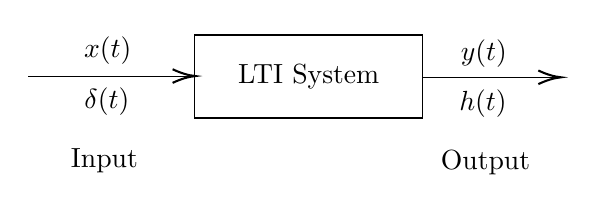
\begin{tikzpicture}[x=0.75pt,y=0.75pt,yscale=-1,xscale=1]
%uncomment if require: \path (0,300); %set diagram left start at 0, and has height of 300

%Shape: Rectangle [id:dp0719812338987873] 
\draw   (140.8,99.8) -- (250.46,99.8) -- (250.46,139.8) -- (140.8,139.8) -- cycle ;
%Straight Lines [id:da4531798525533779] 
\draw    (60.5,119.6) -- (129.02,119.6) -- (139,119.6) ;
\draw [shift={(141,119.6)}, rotate = 180] [color={rgb, 255:red, 0; green, 0; blue, 0 }  ][line width=0.75]    (10.93,-3.29) .. controls (6.95,-1.4) and (3.31,-0.3) .. (0,0) .. controls (3.31,0.3) and (6.95,1.4) .. (10.93,3.29)   ;
%Straight Lines [id:da11632608599684824] 
\draw    (250.46,120.2) -- (315.2,120.2) ;
\draw [shift={(317.2,120.2)}, rotate = 180] [color={rgb, 255:red, 0; green, 0; blue, 0 }  ][line width=0.75]    (10.93,-3.29) .. controls (6.95,-1.4) and (3.31,-0.3) .. (0,0) .. controls (3.31,0.3) and (6.95,1.4) .. (10.93,3.29)   ;

% Text Node
\draw (98.8,107.4) node   [align=left] {$\displaystyle x( t)$};
% Text Node
\draw (98.4,131.8) node   [align=left] {$\displaystyle \delta ( t)$};
% Text Node
\draw (195.63,119.8) node   [align=left] {LTI System};
% Text Node
\draw (280,108.6) node   [align=left] {$\displaystyle y( t)$};
% Text Node
\draw (279.6,133) node   [align=left] {$\displaystyle h( t)$};
% Text Node
\draw (97.2,160.6) node   [align=left] {Input};
% Text Node
\draw (280.8,161.4) node   [align=left] {Output};
\end{tikzpicture}
\end{center}

\subsection{Basic signals}
\begin{enumerate}
    \item Convolution: Delayed impulses
    \item Fourier Analysis: Sinusoidal signals
    \item Laplace Analysis: Complex exponentials
\end{enumerate}

\subsection{Properties of impulse function}
\begin{enumerate}
    \item $x(t)\delta(t-t_0) = x(t_0)\delta(t-t_0)$
    \item $\displaystyle\int_{-\infty}^{\infty} x(t)\delta(t-t_0)\ dt = x(t_0)$
\end{enumerate}

\subsection{Convolution integral}
$$y(t) = \int_{-\infty}^{\infty}x(\tau)h(t-\tau)\ d\tau\Longleftrightarrow\int_{-\infty}^{\infty}x(t-\tau)h(\tau)\ d\tau$$
\begin{itemize}
    \item It can be written as $y(t) = x(t)*h(t)$
\end{itemize}

\subsection{Causal systems}
\begin{itemize}
    \item For causal systems, $h(t) = 0,\ t < 0.\quad \therefore h(t-\tau) = 0,\ t < \tau$
    \item Only past and present values of $x(\tau)$ contribute to $y(t)$.
    \item If $x(t) = 0,\ t < 0$, then the convolution integral of a causal system is
    $$y(t) = \int_0^t x(\tau)h(t-\tau)\ d\tau$$
\end{itemize}

\subsection{Graphical Method}
\begin{enumerate}
    \item Flip: $h(\tau)\rightarrow h(-\tau)$
    \item Shift by $t$: $h(-\tau)\rightarrow h(t-\tau)$
    \item Multiply by $x$: $x(\tau)h(t-\tau)$
    \item Integrate over $\tau$: $\displaystyle y(t) = \int_{-\infty}^{\infty}x(\tau)h(t-\tau)\ d\tau$
\end{enumerate}

\subsection{Properties of Convolution}
\begin{itemize}
    \item Commutative: $x(t)*h(t) = h(t)*x(t)$
    \item Associative: $[x(t)*h_1(t)]*h_2(t) = x(t)*[h_1(t)*h_2(t)]$
    \item Distributive: $x(t)*h_1(t)+x(t)*h_2(t) = x(t)*[h_1(t)+h_2(t)]$
\end{itemize}

\section{W3: Fourier Analysis}
\tikzset{every picture/.style={line width=0.75pt}} %set default line width to 0.75pt        
\begin{center}
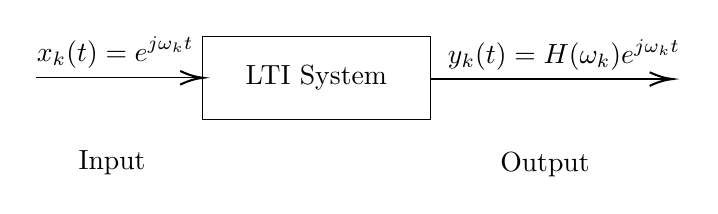
\begin{tikzpicture}[x=0.75pt,y=0.75pt,yscale=-1,xscale=1]
%uncomment if require: \path (0,300); %set diagram left start at 0, and has height of 300

%Shape: Rectangle [id:dp0719812338987873] 
\draw   (140.8,99.8) -- (250.46,99.8) -- (250.46,139.8) -- (140.8,139.8) -- cycle ;
%Straight Lines [id:da4531798525533779] 
\draw    (60.5,119.6) -- (129.02,119.6) -- (139,119.6) ;
\draw [shift={(141,119.6)}, rotate = 180] [color={rgb, 255:red, 0; green, 0; blue, 0 }  ][line width=0.75]    (10.93,-3.29) .. controls (6.95,-1.4) and (3.31,-0.3) .. (0,0) .. controls (3.31,0.3) and (6.95,1.4) .. (10.93,3.29)   ;
%Straight Lines [id:da11632608599684824] 
\draw    (250.46,120.2) -- (365.2,120.2) ;
\draw [shift={(367.2,120.2)}, rotate = 180] [color={rgb, 255:red, 0; green, 0; blue, 0 }  ][line width=0.75]    (10.93,-3.29) .. controls (6.95,-1.4) and (3.31,-0.3) .. (0,0) .. controls (3.31,0.3) and (6.95,1.4) .. (10.93,3.29)   ;

% Text Node
\draw (98.8,107.4) node   [align=left] {$\displaystyle x_k( t) = e^{j\omega_k t}$};
% Text Node
\draw (195.63,119.8) node   [align=left] {LTI System};
% Text Node
\draw (315,108.6) node   [align=left] {$\displaystyle y_k( t) = H(\omega_k)e^{j\omega_k t}$};
% Text Node
\draw (97.2,160.6) node   [align=left] {Input};
% Text Node
\draw (305.8,161.4) node   [align=left] {Output};
\end{tikzpicture}
\end{center}

\subsection{Fourier Series}
\begin{itemize}
    \item A real periodic signal $x(t) = x(t+T_0)$ with period $T_0$ can be expressed as
$$x(t) = \sum_{k=-\infty}^{\infty}a_k e^{jk\omega_0 t},$$
    \begin{itemize}[label=$\circ$]
        \item where $a_k$ is the Fourier coefficients of the Fourier series,
        \item $\omega_0$ is the fundamental frequency of the Fourier series and can be found using the formula:
        $$\omega_0 = \frac{2\pi}{T_0}$$
    \end{itemize}
\end{itemize}
Synthesis: \boxed{x(t) =\sum_{k=-\infty}^{\infty}a_k e^{jk\omega_0 t}}\\
Analysis: \boxed{a_k = \frac{1}{T_0}\int_{T_0}x(t)e^{-jk\omega_0 t}\ dt}
\begin{itemize}
    \item By using the Fourier Analysis formula, we can find the magnitude $|a_k|$ and phase $\theta_k$ of each Fourier coefficient, which can be plotted in the magnitude and phase spectrums respectively.
\end{itemize}

\subsection{Forms of Fourier Series}
\begin{enumerate}
    \item $\displaystyle x(t) =\sum_{k=-\infty}^{\infty}a_k e^{jk\omega_0 t}$
    \item $\displaystyle x(t) = a_0 + 2\sum_{k=1}^{\infty}A_k\cos(k\omega_0 t+\theta_k)$
    \item $\displaystyle x(t) = a_0 + 2\sum_{k=1}^{\infty}[B_k\cos k\omega_0 t-C_k\sin k\omega_0 t]$
\end{enumerate}

\subsection{Fourier Representation of Aperiodic Signals}
\begin{itemize}
    \item $\Tilde{x}(t)$ is $T_0$ periodic, which is made by repeating the aperiodic signal $x(t)$
    \item $\displaystyle \Tilde{x}(t) = \sum_{k=-\infty}^{\infty}a_k e^{jk\omega_0 t}, \ \omega_0 = \frac{2\pi}{T_0}$
    \item As $T_0 \rightarrow \infty,\ \omega_0 \rightarrow 0$
    \item Converges to Fourier Transform
\end{itemize}

\subsection{Power of a signal}
\begin{itemize}
    \item Sum of squares of all the Fourier coefficients
    $$\text{Power} = \sum_{k=-\infty}^{\infty}|a_k|^2 = \frac{1}{T}\int_T |x(t)|^2 \ dt$$
\end{itemize}

\subsection{Periodic x(t)}
\begin{itemize}
    \item Fourier Transform of x(t) is an impulse train
    $$X(\omega) = \sum_{k=-\infty}^{\infty}2\pi a_k \delta(\omega -k\omega_0)$$
\end{itemize}

\subsection{LTI System Response to Exponential Input}
For stable systems:
$$y_{ss}(t) = \int_0^\infty x(\tau)h(t-\tau)\ d\tau = \int_0^\infty x(t-\tau)h(\tau)\ d\tau$$
Given $x(t) = e^{j\omega t}$:
\begin{align*}
    y_{ss}(t) &= \int_0^\infty e^{j\omega(t-\tau)} h(\tau)\ d\tau\\
    &= e^{j\omega t}\int_0^\infty h(\tau) e^{-j\omega\tau}\ d\tau\\
    &= e^{j\omega t}H(\omega)\\
    &= |H(\omega)|e^{j\cdot\text{arg}H(\omega)}e^{j\omega t}\\
    &= |H\omega)|e^{j(\omega t+\text{arg}H(\omega))}
\end{align*}

\subsection{Fourier Transform vs Laplace Transform}
\begin{center}
    Fourier Transform: $\displaystyle \int_{-\infty}^{\infty}x(t)e^{-j\omega t}\ dt$\hspace{1cm} Laplace Transform: $\displaystyle \int_0^\infty x(t)e^{-st}\ dt$
\end{center}
\begin{itemize}
    \item \underline{Limits of Integration:} $-\infty$ to $\infty$ (FT), 0 to $\infty$ (LT)
    \item \underline{Location of complex variable:} $j\omega$ lies on the imaginary axis (FT), \\$s$ can be any complex number in the region of convergence (LT)
    \item \underline{Existence of FT and LT:} If the imaginary axis is not in region of convergence of LT, FT does not exist while LT exists.
    \item \underline{Equivalence of FT and LT:} If $x(t) = 0, t<0$ and imaginary axis is in region of convergence of LT, FT is LT evaluated on the imaginary axis.
    \item \underline{Non-equivalence of FT and LT:} If $x(t) \neq 0 \text{ for } t<0$, then FT $\neq$ LT.
\end{itemize}

\newpage
\section{W4: Modelling Physical Systems}
\subsection{Methodology}
\begin{enumerate}
    \item Draw schematic diagram of system and components, and define variables.
    \item Use physical laws and write equations for each component, combining them together.
    \item Identify unknown system parameters. Thereafter, verify the model with experiments.
\end{enumerate}

\subsection{Translational Mechanical Systems}
\begin{table}[H]
\centering
\begin{tabular}{|l|c|c|c|}
\hline
                      & \textbf{Mass }                                                                                  & \textbf{Spring}                         & \textbf{Damper}                                           \\ \hline
\textbf{Force}                 & $f = m\ddot{x}$                                                                        & $f_k = k(x_2-x_1)$             & $f_b = b(\dot{x}_2-\dot{x}_1)$                   \\ \hline
\textbf{Conservative energies} & \begin{tabular}[c]{@{}c@{}}KE = $\frac{1}{2}m\dot{x}^2$\\ PE = $mgh$\end{tabular} & PE = $\frac{1}{2}kx^2$         & {\color[HTML]{FE0000} \textbf{NOT CONSERVATIVE}} \\ \hline
\textbf{Other laws}            & Power $P = f\dot{x}$                                                           & N2L: $\sum f = ma = m\ddot{x}$ & N3L                                              \\ \hline
\end{tabular}
\end{table}

\subsection{Rotational Mechanical Systems}
\begin{table}[H]
\centering
\begin{tabular}{|l|c|c|c|}
\hline
                               & \textbf{Mass}                     & \textbf{Spring}                            & \textbf{Damper}                                  \\ \hline
\textbf{Torque}                & $\tau = J\ddot{\theta}$           & $\tau_k = k(\theta_2-\theta_1)$            & $\tau_b = b(\dot{\theta}_2-\dot{\theta}_1)$      \\ \hline
\textbf{Conservative energies} & KE = $\frac{1}{2}J\dot{\theta}^2$ & PE = $\frac{1}{2}k\theta^2$                 & {\color[HTML]{FE0000} \textbf{NOT CONSERVATIVE}} \\ \hline
\textbf{Other laws}            & Power $P = \tau\dot{\theta}$      & N2L: $\sum\tau = J\alpha = J\ddot{\theta}$ & N3L                                              \\ \hline
\end{tabular}
\end{table}

\subsection{Energy Method for Mechanical Systems}
\begin{itemize}
    \item Conservative systems only
    \item Do not dissipate energy due to friction
    $$\Delta(\text{KE + PE}) = 0$$
    $$\frac{d}{dt}(\text{KE + PE}) = 0$$
\end{itemize}

\subsection{Electrical Systems}
\begin{table}[H]
\centering\makegapedcells
\begin{tabular}{|l|c|c|c|}
\hline
                               & \textbf{Inductor}                               & \textbf{Capacitor}                            & \textbf{Resistor}                                \\ \hline
\textbf{Current or Voltage}    & $V_a - V_b = L\displaystyle\frac{di_L}{dt}$                  & $i_C = C\displaystyle\frac{d}{dt}(V_a-V_b)$                & $V_a-V_b=i_RR$                                   \\ \hline
\textbf{Conservative energies} & $E_L = \displaystyle\frac{1}{2}Li^2 = \frac{1}{2}L\dot{q}^2$ & $E_C = \frac{1}{2}CV_{ab}^2 = \displaystyle\frac{q^2}{2C}$ & {\color[HTML]{FE0000} \textbf{NOT CONSERVATIVE}} \\ \hline
\textbf{Other laws}            & Power $P = VI$                                  & KVL, KCL                                      & Ohm's Law                                        \\ \hline
\end{tabular}
\end{table}

\newpage
\subsection{Kirchhoff's Laws}
\begin{itemize}
    \item \textbf{Kirchhoff's Voltage Law} (KVL): The algebraic sum of voltages in a loop is zero.
    $$\sum_{i=1}^n V_n = 0$$
    \item \textbf{Kirchhoff's Current Law} (KCL): The algebraic sum of currents entering and leaving the node is zero.
    $$\sum_{i=1}^n I_n = 0$$
\end{itemize}

\subsection{Complex Impedance Method for Electrical Systems}
\begin{itemize}
    \item Ohm's Law: $E(s) = Z(s)I(s)$
    \item Impedances in series: $Z = Z_1+Z_2+Z_3+\cdots$
    \item Impedances in parallel: $Z = \displaystyle\frac{1}{Z_1}+\frac{1}{Z_2}+\frac{1}{Z_2}+\frac{1}{Z_3}+\cdots$
    \item Impedances of electrical components:
\end{itemize}

\begin{table}[H]
\centering\makegapedcells
\begin{tabular}{l|l|l|l|}
\cline{2-4}
                                                  & \multicolumn{1}{c|}{\textbf{Inductor}}                                                      & \multicolumn{1}{c|}{\textbf{Capacitor}}                                                               & \multicolumn{1}{c|}{\textbf{Resistor}}                                                    \\ \hline
\multicolumn{1}{|l|}{\textbf{Current or Voltage}} & $v(t) = L\displaystyle\frac{di(t)}{dt}$                                                                  & $i(t) = C\displaystyle\frac{dv(t)}{dt}$                                                                            & $v(t) = Ri(t)$                                                                            \\ \hline
\multicolumn{1}{|l|}{\textbf{Derivation of Z(s)}} & \begin{tabular}[c]{@{}l@{}}$V(s) = LsI(s)$\\ $Z_L(s) = \displaystyle\frac{V(s)}{I(s)} = Ls$\end{tabular} & \begin{tabular}[c]{@{}l@{}}$I(s) = CsV(s)$\\ $Z_C(s) = \displaystyle\frac{V(s)}{I(s)} = \frac{1}{Cs}$\end{tabular} & \begin{tabular}[c]{@{}l@{}}$V(s) = RI(s)$\\ $Z_R(s) = \displaystyle\frac{V(s)}{I(s)} = R$\end{tabular} \\ \hline
\end{tabular}
\end{table}

\subsection{Op-Amps}
\begin{center}
    Ideal Op-Amp: $e_o = K(e_2-e_1)$
\end{center}
\begin{itemize}
    \item Differential gain of real op-amps: K $\approx 10^5$ to $10^6$
    \item Infinite input impedance
    \item Zero output impedance
    \item Voltage at $e_1$ = Voltage at $e_2$
    \item Current at each input lead is zero
\end{itemize}
\subsubsection{Examples of Op-Amps}
\begin{enumerate}[label=\alph*.]
    \item Inverting amplifier
    \begin{align*}
        G(s) &= \frac{E_o(s)}{E_i(s)} = -\frac{Z_f}{Z_i}
    \end{align*}
    \item Non-inverting amplifier
    \begin{align*}
        G(s) &= \frac{E_o(s)}{E_i(s)} = \frac{Z_1+Z_2}{Z_1}
    \end{align*}
    \item Summing amplifier
    \begin{align*}
        G(s) &= \frac{E_o(s)}{E_i(s)} = -\left(\frac{Z_4}{Z_1}E_1(s)+\frac{Z_4}{Z_2}E_2(s)+\frac{Z_4}{Z_3}E_3(s)\right)
    \end{align*}
\end{enumerate}

\subsection{Analogous Systems}
\begin{itemize}
    \item Physically different systems but sharing the same differential equations and transfer functions
    \item More than 1 mechanical-electrical system analogy
    \begin{itemize}[label=$\circ$]
        \item Spring-Mass $\leftrightarrow$ Series-RLC: Force-Voltage Analogy
\begin{table}[H]
\centering\makegapedcells
\begin{tabular}{|l|l|}
\hline
\textbf{Mechanical System} & \textbf{Electrical System}                          \\ \hline
Force $F$                  & Voltage $V$                                         \\ \hline
Mass $m$                   & Inductance $L$                                      \\ \hline
Damping coefficient $b$    & Resistance $R$                                      \\ \hline
Spring constant $k$        & Reciprocal of capacitance (Elastance) $\displaystyle\frac{1}{C}$ \\ \hline
Displacement $x$           & Charge $q$                                          \\ \hline
Velocity $v$               & Current $i$                                         \\ \hline
\end{tabular}
\end{table}
        \item Spring-Mass $\leftrightarrow$ Parallel-RLC: Mass-Capacitance Analogy
\begin{table}[H]
\centering\makegapedcells
\begin{tabular}{|l|l|}
\hline
\textbf{Mechanical System} & \textbf{Electrical System}                           \\ \hline
Force $F$                  & Current $i$                                          \\ \hline
Mass $m$                   & Capacitance $C$                                      \\ \hline
Damping coefficient $b$    & Reciprocal of resistance (Conductance) $\displaystyle\frac{1}{R}$ \\ \hline
Spring constant $k$        & Reciprocal of inductance $\displaystyle\frac{1}{L}$               \\ \hline
Displacement $x$           & Magnetic flux linkage $\psi$                         \\ \hline
Velocity $v$               & Voltage $V$                                          \\ \hline
\end{tabular}
\end{table}
    \end{itemize}
\end{itemize}

\subsection{Transfer Function (TF)}
$$G(s) = \left.\frac{\mathscr{L}(\text{output})}{\mathscr{L}(\text{input})}\right|_\text{zero initial conditions}$$
$$\text{e.g. }\quad a_0\frac{d^ny}{dt^n}+a_1\frac{d^{n-1}y}{dt^{n-1}}+\ldots+a_{n-1}\frac{dy}{dt}+a_ny = b_0\frac{d^mx}{dt^m}+b_1\frac{d^{m-1}x}{dt^{m=1}}+\ldots+b_{m-1}\frac{dx}{dt}+b_mx$$
\begin{align*}
    \therefore \text{Transfer function, }G(s) &= \left.\frac{\mathscr{L}(y(t))}{\mathscr{L}(x(t))}\right|_\text{zero initial conditions}\\
    &= \frac{Y(s)}{X(s)}\\
    &= \frac{b_0s^m+b_1s^{m-1}+\cdots+b_{m-1}s+b_m}{a_0s^n+a_1s^{n-1}+\cdots+a_{n-1}s+a_n}
\end{align*}
\begin{itemize}
    \item Order of system = highest power of $s$ in denominator
    \item Mathematical model of system
    \item Property of system, unrelated to input
    \item If TF is known, output can be analyzed using inputs to understand systme
    \item If TF is unknown, output can be found by introducing known inputs and studying outputs.
\end{itemize}

\subsection{Impulse-Response Function}
\begin{itemize}
    \item If input $x(t)$ is unit impulse function $\delta(t)$, $X(s) = 1$.
    $$Y(s) = G(s)X(s) = G(s)$$
    \item Transfer function $G(s)$ is the LT of the unit impulse-response function of system $g(t)$:
    $$G(s) = \mathscr{L}(g(t))$$
\end{itemize}

\subsection{Characteristic Equation (CE)}
$$\text{Denominator of TF} = 0$$
\begin{itemize}
    \item Polynomial order $\leftrightarrow$ degree/order of system
    \item Solutions to CE are poles of system
\end{itemize}

\newpage
\section{W5:  First Order Systems}
\subsection{LTI System Response}
\begin{itemize}
    \item Find system response
    \begin{itemize}[label=$\circ$]
        \item Input $\stackrel{\mathrm{TF}}{\longleftrightarrow}$ output
    \end{itemize}
    \item Methods: time domain, frequency domain
    \item Standard input signals:
    \begin{itemize}[label=$\circ$]
        \item Unit impulse
        \item Unit step
        \item Unit ramp
        \item Sine wave
    \end{itemize}
\end{itemize}
\subsection{Parts of System Response}
\begin{itemize}
    \item Transient Response: Immediate response after application of input response
    \item Steady-state Response: Long-time response after application of input response
\end{itemize}
\subsection{Mathematical Model of First Order Systems}
\begin{align*}
    \text{DE: }&\quad T\frac{dy}{dx}+y=Ax\\
    \text{TF: }&\quad \frac{Y(s)}{X(s)} = \frac{A}{Ts+1}
\end{align*}
\begin{itemize}
    \item Time constant/characteristic time: $T$
    \item DC gain: $A$
\end{itemize}
\subsection{Unit Step Response}
\begin{itemize}
    \item Input: $x(t) = u(t)\quad \Rightarrow X(s) = \displaystyle\frac{1}{s}$
    \item Output: $Y(s) = \displaystyle\frac{A}{s(Ts+1)} = A\left(\frac{1}{s}-\frac{1}{s+\frac{1}{T}}\right)$\\
    By ILT: $y(t) = A\left[1-e^{-\frac{t}{T}}\right],\ t\geq 0$
\end{itemize}
\begin{enumerate}
    \item Time constant: $y(T) \approx 0.63A$
    \item Initial speed = $\displaystyle\left.\frac{dy}{dt}\right|_{t = 0} = \frac{A}{T}$
    \item 2\% settling speed: When $y(t_{ss}) = 0.98A,\ t_{ss} = 4T$.
    \item Steady state error, $e_{ss} = \displaystyle\lim_{t\to\infty}\left[u(t)-y(t)\right] = 1-A$
\end{enumerate}
\subsection{Unit Impulse Response}
\begin{itemize}
    \item Input: $x(t) = \delta(t)\quad \Rightarrow X(s) = 1$
    \item Output: $Y(s) = \displaystyle\frac{A}{Ts+1} = \frac{A}{T}\left(\frac{1}{s+\frac{1}{T}}\right)$\\
    By ILT: $y(t) = \displaystyle\frac{A}{T}e^{-\frac{t}{T}},\ t\geq 0$
\end{itemize}
\begin{enumerate}
    \item Time constant: $y(t) \approx 0.37A$
    \item Initial speed = $\displaystyle\left.\frac{dy}{dt}\right|_{t=0} = -A$
    \item Steady state error, $e_{ss} = \displaystyle\lim_{t\to\infty}\left[\delta(t)-y(t)\right] = \displaystyle\lim_{t\to\infty}\left[-\displaystyle\frac{A}{T}e^{-\frac{t}{T}}\right] = 0$
\end{enumerate}
\subsection{Unit Ramp Response}
\begin{itemize}
    \item Input: $x(t) = t\quad \Rightarrow X(s) = \displaystyle\frac{1}{s^2}$
    \item Output: $Y(s) = \displaystyle\frac{A}{s^2(Ts+1)} = \frac{A}{s^2}-\frac{AT}{s}+\frac{AT^2}{Ts+1}$\\
    By ILT: $y(t) = At-AT+ATe^{-\frac{t}{T}},\ t\geq 0$
\end{itemize}
\begin{enumerate}
    \item Initial speed = $\displaystyle\left.\frac{dy}{dt}\right|_{t=0} = A-Ae^{-\frac{t}{T}}$
    \item Steady state error, $e_{ss} = \displaystyle\lim_{t\to\infty}\left[r(t)-y(t)\right]=\displaystyle\lim_{t\to\infty}\left[t-AT\left(\displaystyle\frac{t}{T}-1+e^{-\frac{t}{T}}\right)\right] = AT+\displaystyle\lim_{t\to\infty}\left[t(1-A)\right]$
\end{enumerate}
\subsection{Responses of First Order Systems}
\begin{itemize}
    \item Unit ramp function, $r(t)$: $y_r(t) = AT\left(\frac{t}{T}-1+e^{-\frac{t}{T}}\right),\ t\geq 0$
    \item Unit step function, $u(t)$: $y_u(t) = A(1-e^{-\frac{t}{T}}),\ t\geq 0$
    \item Unit impulse function, $\delta(t)$: $y_\delta(t) =\displaystyle\frac{A}{T}e^{-\frac{t}{T}},\ t\geq 0$
    \item Properties:
    \begin{itemize}[label=$\circ$]
        \item $\displaystyle\frac{d}{dt}y_r(t) = y_u(t)$
        \item $\displaystyle\frac{d}{dt}y_u(t) = y_\delta(t)$
        \item Applies to higher order systems as well
    \end{itemize}
\end{itemize}
\subsection{Responses of First-Order Systems in Frequency and Time Domains}
\begin{table}[H]
\centering\makegapedcells
\begin{tabular}{|c|c|c|l|l|}
\hline
\multicolumn{2}{|c|}{\multirow{2}{*}{$T \displaystyle\frac{dy(t)}{dt}+y(t) = Ax(t)$}}                                                                          & \multicolumn{3}{c|}{\textbf{Response to}}                                                                                                                                                                                                                                                                                                                                                                                                                                                             \\ \cline{3-5} 
\multicolumn{2}{|c|}{}                                                                                                                                         & \textbf{Unit step}                                                                                                                                                     & \multicolumn{1}{c|}{\textbf{Unit impulse}}                                                                                                           & \multicolumn{1}{c|}{\textbf{Unit ramp}}                                                                                                                               \\ \hline
\multicolumn{2}{|c|}{\begin{tabular}[c]{@{}c@{}}\textbf{Frequency domain:}\\ \\ Transfer function\\ $H(s) = \displaystyle\frac{A}{Ts+1}$\end{tabular}}                  & \multicolumn{1}{l|}{\begin{tabular}[c]{@{}l@{}}$X(s)= \displaystyle\frac{1}{s}$\\ $Y(s)= H(s)X(s)$\\ $\qquad = \displaystyle\frac{A}{s}-\frac{AT}{Ts+1}$\end{tabular}} & \begin{tabular}[c]{@{}l@{}}$X(s) = 1$\\ $Y(s) = H(s)X(s)$\\ $\qquad= \displaystyle\frac{A}{Ts+1}$\end{tabular}                                       & \begin{tabular}[c]{@{}l@{}}$X(s) = \displaystyle\frac{1}{s^2}$\\ $Y(s) = H(s)X(s)$\\ $\qquad= \displaystyle\frac{A}{s^2}-\frac{AT}{s}+\frac{AT^2}{Ts+1}$\end{tabular} \\ \hline
\multicolumn{2}{|c|}{\begin{tabular}[c]{@{}c@{}}\textbf{Time domain:}\\ \\ Impulse response\\ $h(t) = \displaystyle\frac{A}{T}e^{-\frac{t}{T}},\ t\geq 0$\end{tabular}} & \multicolumn{1}{l|}{\begin{tabular}[c]{@{}l@{}}$x(\tau) = u(\tau)$\\ $y(t) = h(t)\ast x(t)$\\ $\qquad = A\left(1-e^{-\frac{t}{T}}\right),\ t\geq 0$\end{tabular}}      & \begin{tabular}[c]{@{}l@{}}$x(\tau) = \delta(\tau)$\\ $y(t) = h(t)\ast x(t)$\\ $\qquad = \displaystyle{A}{T}e^{-\frac{t}{T}},\ t\geq 0$\end{tabular} & \begin{tabular}[c]{@{}l@{}}$x(\tau) = \tau$\\ $y(t) = h(t)\ast x(t)$\\ $\qquad = A\left(t-T+Te^{-\frac{t}{T}}\right),\ t\geq 0$\end{tabular}                          \\ \hline
\multicolumn{1}{|l|}{\textbf{Poles}}                                              & $s = -\displaystyle\frac{1}{T}$                                            & $s = 0,\ s = \displaystyle -\frac{1}{T}$                                                                                                                               & \multicolumn{1}{c|}{$s = \displaystyle -\frac{1}{T}$}                                                                                                & \multicolumn{1}{c|}{$s = 0,\ s = 0,\ s = \displaystyle -\frac{1}{T}$}                                                                                                 \\ \hline
\end{tabular}
\end{table}

\newpage
\section{W5 \& W6: Second Order Systems}
\subsection{General form of Second Order Systems}
$$G(s) = \displaystyle\frac{\omega_n^2}{s^2+2\zeta\omega_n s+\omega_n^2},$$
\begin{itemize}
    \item where $\zeta$ is the damping ratio and $\omega_n$ is the natural frequency of the system.
    \item Characteristic equation: $s^2+2\zeta\omega_n s +\omega_n^2 = 0$
    \item Poles: $s_1 = -\zeta\omega_n+\omega_n\sqrt{\zeta^2-1},\ s_2 = -\zeta\omega_n-\omega_n\sqrt{\zeta^2-1}$
\end{itemize}

\subsection{Parameters of Second Order Systems}
\begin{itemize}
    \item The poles of second order systems can be rewritten as:
    \begin{align*}
        s_{1,2} &= -\zeta\omega_n\pm\omega_n\sqrt{\zeta^2-1}= -\zeta\omega_n\pm j\omega_n\sqrt{1-\zeta^2}\\
        &= -\sigma\pm j\omega_d
    \end{align*}
    \begin{itemize}[label=$\circ$]
        \item where $\sigma$ is the attenuation of the system, \quad \boxed{\sigma = \zeta\omega_n}
        \item and $\omega_d$ is the damped natural frequency of the system. \quad \boxed{\omega_d = \omega_n\sqrt{1-\zeta^2}}
    \end{itemize}
    \item For physical systems, the natural frequency $\omega_n$ is always positive. 
\end{itemize}

\subsection{Effects of Damping Ratio on Natural Response of Second Order Systems}
\begin{itemize}
    \item Case 1: Unstable ($\sigma < 0,\ \zeta < 0$)
    \item Case 2: Marginally stable, undamped conjugate complex poles ($\sigma = 0,\ \zeta = 0$)
    \item Case 3a: Stable, underdamped, conjugate complex poles ($0<\zeta<1$)
    \item Case 3b: Stable, critically damped, repeated real poles ($\zeta = 1$)
    \item Case 3c: Stable, overdamped, distinct real poles ($\zeta > 1$)
\end{itemize}

\subsection{Natural Response of Second Order Systems}
We have a generic second order equation of motion.
$$\ddot{x}+2\zeta\omega_n\dot{x}+\omega_n^2x = 0$$
Taking the Laplace Transform of it:
\begin{center}
    $s^2X(s)-sx(0) -\dot{x}(0)+2\zeta\omega_n[sX(s)-x(0)]+\omega_n^2X(s) = 0$\vspace{0.1cm}\\
    $\therefore X(s) = \displaystyle\frac{sx(0)+2\zeta\omega_n x(0)+\dot{x}(0)}{s^2+2\zeta\omega_n s+\omega_n^2}$
\end{center}
For the same set of initial conditions $x(0)$, $\displaystyle\frac{dx(0)}{dt}$ and $\omega_n$, the free response of the system can be different based on the value of the damping ratio $\zeta$.

\subsubsection{Natural Response of Marginally Stable, Underdamped System (Case 2)}
\begin{align*}
    X(s) &= \frac{sx(0)+\dot{x}(0)}{s^2+\omega_n^2}\\
    &= x(0)\frac{s}{s^2+\omega_n^2}+\frac{\dot{x}(0)}{\omega_n}\frac{\omega_n}{s^2+\omega_n^2}
\end{align*}
Taking ILT:
$$x(t) = x(0)\cos\omega_n t+\left(\frac{\dot{x}(0)}{\omega_n}\right)\sin\omega_n t,\ t\geq 0$$

\subsubsection{Natural Response of Stable, Underdamped System (Case 3a)}
\begin{align*}
    X(s) &= \frac{sx(0)+2\zeta\omega_n x(0)+\dot{x}(0)}{s^2+2\zeta\omega_n s+\omega_n^2}\\
    &= \frac{sx(0)+2\zeta\omega_n x(0)+\dot{x}(0)}{(s+\zeta\omega_n)^2+(\omega_n\sqrt{1-\zeta^2})^2}\\
    &= \left(\frac{\zeta\omega_n x(0)+\dot{x}(0)}{\omega_n\sqrt{1-\zeta^2}}\right)\frac{\omega_n\sqrt{1-\zeta^2}}{(s+\zeta\omega_n)^2+(\omega_n\sqrt{1-\zeta^2})^2} + x(0)\frac{s+\zeta\omega_n}{(s+\zeta\omega_n)^2+(\omega_n\sqrt{1-\zeta^2})^2}
\end{align*}
Taking ILT:
\begin{align*}
    x(t) &= \left(\frac{\zeta\omega_n x(0)+\dot{x}(0)}{\omega_n\sqrt{1-\zeta^2}}\right)e^{-\zeta\omega_n t}\sin(\omega_n\sqrt{1-\zeta^2}t)+x(0)e^{-\zeta\omega_n t}\cos(\omega_n\sqrt{1-\zeta^2}t),\ t > 0\\
    &= e^{-\zeta\omega_n t}\left\{\left[\frac{\zeta}{\sqrt{1-\zeta^2}}x(0)+\frac{1}{\omega_d}\dot x(0)\right]\sin\omega_d t + x(0)\cos\omega_d t\right\},\ t > 0
\end{align*}
The system oscillates at the damping frequency $\omega_d$.

\subsubsection{Natural Response of Stable, Critically Damped System (Case 3b)}
\begin{align*}
    X(s) &= \frac{sx(0)+2\omega_n x(0)+\dot{x}(0)}{s^2+2\omega_n s+\omega_n^2}\\
    &= \frac{x(0)}{s+\omega_n} + \frac{\omega_n x(0)+\dot{x}(0)}{(s+\omega_n)^2}
\end{align*}
Taking ILT:
\begin{align*}
    x(t) = x(0)e^{-\omega_n t}+\left[\omega_n x(0)+\dot{x}(0)\right]te^{-\omega_n t},\ t>0
\end{align*}

\subsubsection{Natural Response of Stable, Overdamped System (Case 3c)}
\begin{align*}
    X(s) &= \frac{sx(0)+2\omega_n x(0)+\dot{x}(0)}{s^2+2\zeta\omega_n s+\omega_n^2}\\
    &= \frac{(s+2\zeta\omega_n)x(0)+\dot{x}(0)}{(s+\zeta\omega_n+\omega_n\sqrt{\zeta^2-1})(s+\zeta\omega_n-\omega_n\sqrt{\zeta^2-1})}\\
    &= \frac{\hat{a}}{(s+\zeta\omega_n+\omega_n\sqrt{\zeta^2-1})}+\frac{\hat{b}}{(s+\zeta\omega_n-\omega_n\sqrt{\zeta^2-1})}
\end{align*}
Taking ILT:
\begin{align*}
    x(t) = \hat{a}e^{-(\zeta\omega_n+\omega_n\sqrt{\zeta^2-1})}+\hat{b}e^{-(\zeta\omega_n-\omega_n\sqrt{\zeta^2-1})},\ t>0
\end{align*}
    $$\text{where }\hat{a} = \frac{x(0)(-\zeta+\sqrt{\zeta^2-1})}{2\sqrt{\zeta^2-1}}-\frac{\dot{x}(0)}{2\omega_n\sqrt{\zeta^2-1}},\qquad\hat{b} = \frac{x(0)(\zeta+\sqrt{\zeta^2-1})}{2\sqrt{\zeta^2-1}}-\frac{\dot{x}(0)}{2\omega_n\sqrt{\zeta^2-1}}$$

\subsection{Comparison of Natural Response of Stable Systems (Cases 3a, 3b, 3c)}
\begin{itemize}
    \item If the poles of X(s) are stable, steady state value of $x(t)$ can be computed:
    \begin{align*}
        x(t\to\infty) &= \lim_{s\to 0} sX(s)\\
        &= \lim_{s\to 0}\frac{s^2x(0)+2\zeta\omega_n x(0)+\dot{x}(0)s}{s^2+2\zeta\omega_n s+\omega_n^2}\\
        &= 0
    \end{align*}
    \item For Cases 3a, 3b and 3c, their responses return to equilibrium position as $t\to \infty$.
\end{itemize}

\subsection{Logarithmic Decrement Method}
\begin{itemize}
    \item Used to find the damping ratio $\zeta$.
    \item Procedure:
    \begin{enumerate}
        \item Find the amplitude of the first peak $x_1$ and that of the nth peak $x_n$.
        \item The logarithmic decrement $\delta$ can be found using the formula:
        $$\delta = \frac{1}{n-1}\ln \frac{x_1}{x_n}$$
        \item The damping ratio $\zeta$ can be found by applying this formula:
        $$\zeta = \frac{\delta}{\sqrt{4\pi^2+\delta^2}}$$
    \end{enumerate}
\end{itemize}

\subsection{Unit Step Response of Second Order Systems}
The transfer function $G(s)$ of a second order system is as follows:
$$G(s) = \frac{C(s)}{R(s)} = \frac{\omega_n^2}{s^2+2\zeta\omega_n s+\omega_n^2}$$
If $R(s)$ is a unit step input, $R(s) = \displaystyle\frac{1}{s}$.
\begin{align*}
    C(s) &= R(s)G(s)\\
    &= \frac{\omega_n^2}{s(s^2+2\zeta\omega_n s+\omega_n^2)}\\
    &= \frac{1}{s}-\frac{s+2\zeta\omega_n}{s^2+2\zeta\omega_n s+\omega_n^2}
\end{align*}
The unit step response of the system $c(t)$ depends on the poles of $C(s)$.

\subsubsection{Unit Step Response of Marginally Stable, Underdamped System (Case 2)}
$$C(s) = \frac{1}{s}-\frac{s}{s^2+\omega_n^2}$$
Taking ILT,
$$c(t) = u(t)-\cos \omega_n t,\ t>0$$

\subsubsection{Unit Step Response of Stable, Underdamped System (Case 3a)}
\begin{align*}
    C(s) &= \frac{1}{s}-\frac{s+2\zeta\omega_n}{s^2+2\zeta\omega_n s+\omega_n^2}\\
    &= \frac{1}{s}-\frac{s+\zeta\omega_n}{(s+\zeta\omega_n)^2+\omega_d^2}-\frac{\zeta\omega_n}{(s+\zeta\omega_n)^2+\omega_d^2}
\end{align*}
Taking ILT,
$$c(t) = u(t)-e^{-\zeta\omega_n t}\left[\cos\omega_d t+\frac{\zeta}{\sqrt{1-\zeta^2}}\sin\omega_d t\right],\ t>0$$

\subsubsection{Unit Step Response of Stable, Critically Damped System (Case 3b)}
\begin{align*}
    C(s) &= \frac{\omega_n^2}{s(s^2+2\omega_n s+\omega_n)}\\
    &= \frac{\omega_n^2}{s(s+\omega_n)^2}\\
    &= \frac{1}{s}-\frac{1}{s+\omega_n}-\frac{\omega_n}{(s+\omega_n)^2}
\end{align*}
Taking ILT,
\begin{align*}
    c(t) &= u(t)-e^{-\omega_n t}-\omega_n te^{-\omega_n t}\\
    &= u(t) - e^{-\omega_n t}(1+\omega_n t),\ t>0
\end{align*}

\subsubsection{Unit Step Response of Stable, Overdamped System (Case 3c)}
\begin{align*}
    C(s) &= \frac{\omega_n^2}{s(s^2+2\omega_n s+\omega_n)}\\
    &= \frac{\omega_n^2}{s(s+\zeta\omega_n+\omega_n\sqrt{\zeta^2-1})(s+\zeta\omega_n-\omega_n\sqrt{\zeta^2-1})}\\
    &= \frac{1}{s}+\frac{\Bar{a}}{s+\omega_n(\zeta+\sqrt{\zeta^2-1})}+\frac{\Bar{b}}{s+\omega_n(\zeta-\sqrt{\zeta^2-1})}
\end{align*}
Taking ILT,
\begin{align*}
    c(t) = u(t)+\Bar{a}e^{-\omega_n t(\zeta+\sqrt{\zeta^2-1})}+\Bar{b}e^{-\omega_n t(\zeta-\sqrt{\zeta^2-1})},\ t>0
\end{align*}
$$\text{where }\Bar{a}=\frac{1}{2\sqrt{\zeta^2-1}(\zeta+\sqrt{\zeta^2-1})},\ \qquad\Bar{b}=-\frac{1}{2\sqrt{\zeta^2-1}(\zeta-\sqrt{\zeta^2-1})}$$

\subsection{Comparison of Unit Step Response for Stable Systems (Cases 3a, 3b, 3c)}
\begin{itemize}
    \item If the poles of C(s) are stable, steady state value of $c(t)$ can be computed:
    \begin{align*}
        c(t\to\infty)&= \lim_{s\to 0}sC(s)\\
        &= \lim_{s\to 0}\frac{\omega_n^2}{s^2+2\zeta\omega_n s+\omega_n^2}\\
        &= 1
    \end{align*}
    \item For Cases 3a, 3b and 3c, their responses tend to 1 as $t\to\infty$.
    \item Among underdamped systems (Case 3a), systems with $0.5<\zeta<0.8$ converges the quickest.
    \item Critically damped systems (Case 3b) exhibits the fastest response for all values of $\zeta$.
    \item Overdamped systmes (Case 3c) converges to the steady-state value without oscillating.
\end{itemize}

\subsection{Transient Parameters of Second Order Systems}
\begin{itemize}
    \item Standard initial conditions of zero and unit-step input $r(t) = u(t)$ are used as common practice.
\end{itemize}
\begin{enumerate}
    \item \textbf{Delay time}, $t_d$: Time required for response to reach 50\% of final value the first time.
    \item \textbf{Rise time}, $t_r$: Time required for response to rise from 0\% to 100\% of the final value.
    $$t_r = \frac{1}{\omega_d}\tan^{-1}\left(\frac{\omega_d}{-\sigma}\right) = \frac{\pi-\beta}{\omega_d}$$
    \item \textbf{Peak time}, $t_p$: Time required for response to reach first peak of overshoot
    $$t_p = \frac{\pi}{\omega_d}$$
    \item \textbf{Maximum (Percent) Overshoot}, $M_p$: Maximum peak value of response measured from steady state value
    \begin{align*}
        M_p &= \frac{c(t_p)-c(\infty)}{c(\infty)}\quad &M_p(\%)&= \frac{c(t_p)-c(\infty)}{c(\infty)}\\
        &= e^{-\displaystyle\frac{\zeta\pi}{\sqrt{1-\zeta^2}}}\quad&&= e^{-\displaystyle\frac{\zeta\pi}{\sqrt{1-\zeta^2}}}\times100\%
    \end{align*}
    \item \textbf{Settling time}, $t_s$: Time required for response to reach and stay within 2\% or 5\% of the final value
    \begin{align*}
        t_s &= 4T = \frac{4}{\zeta\omega_n}\quad (2\%)\\
        t_s &= 3T = \frac{3}{\zeta\omega_n}\quad (5\%)
    \end{align*}
\end{enumerate}

\subsection{Higher Order Systems}
\begin{itemize}
    \item Unit step response of higher order systems will be a linear sum of first order and second order systems
\end{itemize}

\subsection{Dominant Poles}
\begin{itemize}
    \item Slowest poles of systems are responsible for longest lasting terms in transient response.
    \item Let $-p$ be the first order pole and $-\zeta\omega_n$ be the second order pole.
\end{itemize}

\subsubsection{Dominant First Order Behaviour}
\begin{itemize}
    \item If $\zeta\omega_n \geq 10p$, then $G(s) \approx \displaystyle\frac{\frac{K}{\omega_n^2}}{s+p}$.
\end{itemize}

\subsubsection{Dominant Second Order Behaviour}
\begin{itemize}
    \item If $p\geq 10\zeta\omega_n$, then $G(s)\approx\displaystyle\frac{\frac{K}{p}}{s^2+2\zeta\omega_n s+\omega_n^2}$.
\end{itemize}

\newpage
\section{W8: Fluid \& Thermal Systems}

\subsection{Introduction to Fluid Systems}
\begin{itemize}
    \item 2 main types of fluid systems: 
    \begin{itemize}[label=$\circ$]
        \item Hydraulic systems (containing liquids) 
        \item Pneumatic systems (containing gases)
    \end{itemize} 
    \item 2 types of fluid flow:
    \begin{itemize}[label=$\circ$]
        \item Laminar flow (viscous forces dominate)
        \item Turbulent flow (inertial forces dominate)
    \end{itemize}
\end{itemize}

\subsection{Parameters of Fluid Flow}
\begin{itemize}
    \item \textbf{Fluid Resistance}, $R$: measure of change in pressure required to change unit change in flow rate
    $$R = \frac{\Delta\text{ Pressure}}{\Delta\text{ Flow rate}}=\frac{dP}{dQ}$$
    \item \textbf{Fluid Capacitance}, $C$: measure of change in stored fluid required to cause unit change in pressure
    $$C = \frac{\Delta\text{ Capacity}}{\Delta\text{ Pressure}}=\frac{Q\ dt}{dP}$$
    \begin{itemize}[label=$\circ$]
        \item With a constant cross-sectional area $A$:
        $$C = \frac{\Delta\text{ Capacity}}{\Delta\text{ Pressure Head}}=\frac{Q\ dt}{dh}$$
    \end{itemize}
    \item \textbf{Fluid Inductance}, $I$: measure of change in pressure to make unit rate of change in the flow rate
    $$I = \frac{\Delta\text{ Pressure}}{\text{Rate of change of flow rate}} = \frac{dP\ dt}{dQ}$$
    \begin{itemize}[label=$\circ$]
        \item Negligible in liquid systems
    \end{itemize}
\end{itemize}

\subsection{Modelling Liquid Level Systems}
\begin{itemize}
    \item Fluid inductance neglected.
    \item Assign variables to flow rates and pressure/pressure head.
    \item Using continuity of flow, conservation of mass and Newton's 2nd Law, write equations for each parameter.
    \item Useful equations:
    \begin{itemize}[label=$\circ$]
        \item Continuity of flow: Fluid accumulated = Net inflow of fluid
        $$C\frac{dh}{dt} = q_i-q_o$$
        \item Fluid resistance: $\displaystyle R =\frac{dh}{dQ}$
        \item Power = $P\times Q$
    \end{itemize}
\end{itemize}

\subsection{Modelling Hydraulic Systems}
\begin{itemize}
    \item Assume hydraulic fluid is incompressible.
    \item Fluid inductance neglected.
    \item Assign variables to mass flow rates, pressure, displacement and velocities.
    \item Using continuity of flow, conservation of mass and Newton's 2nd Law, write equations for each parameter,
    \item Useful equations:
    \begin{itemize}[label=$\circ$]
        \item Continuity of flow: Fluid passing throgugh piston = Movement of piston
        $$q = \rho A(\dot{y}-\dot{z})$$
        \item Fluid resistance: $R = \displaystyle\frac{dP}{dQ}$
        \item Power = $P\times Q$
    \end{itemize}
\end{itemize}

\subsection{Modelling Pneumatic Systems}
\begin{itemize}
    \item Assume subsonic fluid flow.
    \item Fluid inductance neglected.
    \item Assign variables to mass flow rates and pressure.
    \item Using continuity of flow, conservation of mass and Newton's 2nd Law, write equations for each parameter.
    \item Useful equations:
    \begin{itemize}[label=$\circ$]
        \item Continuity of flow: Fluid accumulated = Net inflow of fluid
        $$C\frac{dp_o}{dt} = q$$
        \item Fluid resistance: $\displaystyle R = \frac{dP}{dQ} = \frac{p_i-p_o}{q}$
        \item Power = $P\times Q$
    \end{itemize}
\end{itemize}

\subsection{Introduction to Thermal Systems}
\begin{itemize}
    \item 3 modes of heat transfer:
    \begin{itemize}[label=$\circ$]
        \item Conduction
        \item Convection
        \item Radiation (negligible unless very high temperatures)
    \end{itemize}
    \item Rate of heat flow for conductive and convective heat transfer, $q = K\Delta\theta$
    \begin{itemize}[label=$\circ$]
        \item where $K$ is the heat transfer coefficient and $\Delta\theta$ is the temperature difference between the two mediums.
    \end{itemize}
\end{itemize}

\subsection{Parameters of Heat Flow}
\begin{itemize}
    \item \textbf{Thermal Resistance}, $R$: \\measure of the change in temperature difference required to cause a unit change in heat flow rate
    $$R = \frac{\Delta\text{ Temperature difference}}{\Delta\text{ Heat flow rate}} = \frac{d(\Delta\theta)}{dq} = \frac{1}{K}$$
    \item \textbf{Thermal Capacitance}, $C$: measure of the change in quantity of heat energy stored required to cause a unit change in temperature
    $$C = \frac{\Delta\text{ Heat energy capacity}}{\Delta\text{ Temperature}} = \frac{q\ dt}{d\theta}$$
\end{itemize}

\subsection{Modelling Thermal Systems}
\begin{itemize}
    \item Assign variables to heat flow rates and temperature.
    \item Using continuity of heat flow and conservation of energy, write equations for each parameter.
    \item Useful equations:
    \begin{itemize}
        \item Continuity of heat flow: $q = \displaystyle C\frac{d\theta}{dt}$
        \item Thermal resistance: $R = \displaystyle\frac{d(\Delta\theta)}{dq} = \frac{\theta_a-\theta_b}{q}$
        \item Power = $\theta\times q$
    \end{itemize}
\end{itemize}

\newpage
\section{W8: Block Diagrams}
\tikzset{every picture/.style={line width=0.75pt}} %set default line width to 0.75pt        
\begin{center}
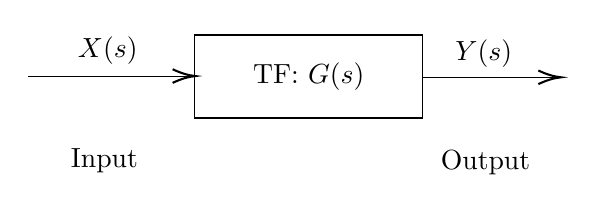
\begin{tikzpicture}[x=0.75pt,y=0.75pt,yscale=-1,xscale=1]
%uncomment if require: \path (0,300); %set diagram left start at 0, and has height of 300

%Shape: Rectangle [id:dp0719812338987873] 
\draw   (140.8,99.8) -- (250.46,99.8) -- (250.46,139.8) -- (140.8,139.8) -- cycle ;
%Straight Lines [id:da4531798525533779] 
\draw    (60.5,119.6) -- (129.02,119.6) -- (139,119.6) ;
\draw [shift={(141,119.6)}, rotate = 180] [color={rgb, 255:red, 0; green, 0; blue, 0 }  ][line width=0.75]    (10.93,-3.29) .. controls (6.95,-1.4) and (3.31,-0.3) .. (0,0) .. controls (3.31,0.3) and (6.95,1.4) .. (10.93,3.29)   ;
%Straight Lines [id:da11632608599684824] 
\draw    (250.46,120.2) -- (315.2,120.2) ;
\draw [shift={(317.2,120.2)}, rotate = 180] [color={rgb, 255:red, 0; green, 0; blue, 0 }  ][line width=0.75]    (10.93,-3.29) .. controls (6.95,-1.4) and (3.31,-0.3) .. (0,0) .. controls (3.31,0.3) and (6.95,1.4) .. (10.93,3.29)   ;

% Text Node
\draw (98.8,107.4) node   [align=left] {$\displaystyle X(s)$};
% Text Node
\draw (195.63,119.8) node   [align=left] {TF: $G(s)$};
% Text Node
\draw (280,108.6) node   [align=left] {$\displaystyle Y(s)$};
% Text Node
\draw (97.2,160.6) node   [align=left] {Input};
% Text Node
\draw (280.8,161.4) node   [align=left] {Output};
\end{tikzpicture}
\end{center}

\begin{itemize}
    \item Pictorial representation of system
    \item Variables linked to each other via TF blocks
    \item Signals travel in direction of arrow
    \item Systems can share same block diagram
\end{itemize}

\subsection{Elements of A Block Diagram}
\begin{itemize}
    \item \textbf{Block}: represents the transfer function of a system component, with a single input and a single output
    \item \textbf{Summing point}: represents point of a system component, with more than 1 input and a single output 
    \item \textbf{Branch point}: represents the point where the signal from one block goes to other blocks or summing points at the same time
\end{itemize}

\subsection{Feedback Loop Transfer Functions}
\begin{center}
\tikzset{every picture/.style={line width=0.75pt}} %set default line width to 0.75pt        

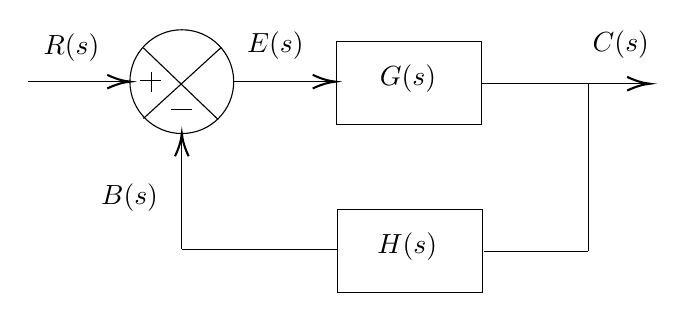
\begin{tikzpicture}[x=0.75pt,y=0.75pt,yscale=-1,xscale=1]
%uncomment if require: \path (0,515); %set diagram left start at 0, and has height of 515

%Shape: Circle [id:dp4181485712735933] 
\draw   (100,149) .. controls (100,135.19) and (111.19,124) .. (125,124) .. controls (138.81,124) and (150,135.19) .. (150,149) .. controls (150,162.81) and (138.81,174) .. (125,174) .. controls (111.19,174) and (100,162.81) .. (100,149) -- cycle ;
%Straight Lines [id:da4740649733052047] 
\draw    (51,149) -- (98,149) ;
\draw [shift={(100,149)}, rotate = 180] [color={rgb, 255:red, 0; green, 0; blue, 0 }  ][line width=0.75]    (10.93,-3.29) .. controls (6.95,-1.4) and (3.31,-0.3) .. (0,0) .. controls (3.31,0.3) and (6.95,1.4) .. (10.93,3.29)   ;
%Straight Lines [id:da3499230348244544] 
\draw    (150,149) -- (197,149) ;
\draw [shift={(199,149)}, rotate = 180] [color={rgb, 255:red, 0; green, 0; blue, 0 }  ][line width=0.75]    (10.93,-3.29) .. controls (6.95,-1.4) and (3.31,-0.3) .. (0,0) .. controls (3.31,0.3) and (6.95,1.4) .. (10.93,3.29)   ;
%Shape: Rectangle [id:dp720053978182877] 
\draw   (199.5,129.5) -- (269.5,129.5) -- (269.5,169.5) -- (199.5,169.5) -- cycle ;
%Straight Lines [id:da444930263203553] 
\draw    (269.5,150) -- (348.5,150) ;
\draw [shift={(350.5,150)}, rotate = 180] [color={rgb, 255:red, 0; green, 0; blue, 0 }  ][line width=0.75]    (10.93,-3.29) .. controls (6.95,-1.4) and (3.31,-0.3) .. (0,0) .. controls (3.31,0.3) and (6.95,1.4) .. (10.93,3.29)   ;
%Straight Lines [id:da11472626901203187] 
\draw    (321,150.25) -- (321,230.75) ;
%Straight Lines [id:da39388134421732124] 
\draw    (270.5,230.75) -- (320.5,230.75) ;
%Shape: Rectangle [id:dp21026770917278692] 
\draw   (200,210.5) -- (270,210.5) -- (270,250.5) -- (200,250.5) -- cycle ;
%Straight Lines [id:da4509078916088618] 
\draw    (125,229.75) -- (200,229.75) ;
%Straight Lines [id:da2451181139005163] 
\draw    (125,229.75) -- (125,176) ;
\draw [shift={(125,174)}, rotate = 450] [color={rgb, 255:red, 0; green, 0; blue, 0 }  ][line width=0.75]    (10.93,-3.29) .. controls (6.95,-1.4) and (3.31,-0.3) .. (0,0) .. controls (3.31,0.3) and (6.95,1.4) .. (10.93,3.29)   ;
%Straight Lines [id:da9337473628239266] 
\draw    (106.5,132.75) -- (142.5,167.25) ;
%Straight Lines [id:da5043252444487525] 
\draw    (144,132.5) -- (106.5,166.75) ;
%Straight Lines [id:da8451547864563302] 
\draw    (105,148.5) -- (115,148.5) ;
%Straight Lines [id:da7484338496828458] 
\draw    (110.5,144.25) -- (110.5,153.75) ;
%Straight Lines [id:da9743377983002497] 
\draw    (120,162.5) -- (130,162.5) ;

% Text Node
\draw (57.14,124.69) node [anchor=north west][inner sep=0.75pt]    {$R( s)$};
% Text Node
\draw (155.14,123.54) node [anchor=north west][inner sep=0.75pt]    {$E( s)$};
% Text Node
\draw (219.14,139.54) node [anchor=north west][inner sep=0.75pt]    {$G( s)$};
% Text Node
\draw (321.71,123.26) node [anchor=north west][inner sep=0.75pt]    {$C( s)$};
% Text Node
\draw (218,220.69) node [anchor=north west][inner sep=0.75pt]    {$H( s)$};
% Text Node
\draw (84.86,196.69) node [anchor=north west][inner sep=0.75pt]    {$B( s)$};
\end{tikzpicture}\\
This is a \textcolor{red}{\textbf{NEGATIVE}} feedback loop.
\end{center}

\begin{itemize}
    \item Parameters:
    \begin{itemize}[label=$\circ$]
        \item $R(s)$: input
        \item $E(s)$: error
        \item $C(s)$: output
        \item $B(s)$: feedback
    \end{itemize}
    \item \textbf{Open Loop Transfer Function} (OLTF): ratio of feedback signal to error signal
    $$\text{OLTF} = \frac{B(s)}{E(s)} = G(s)H(s)$$
    \item \textbf{Feedforward Transfer Function} (FTF): ratio of output signal to error signal
    $$\text{FTF} = \frac{C(s)}{E(s)} = G(s)$$
    \item \textbf{Negative Closed Loop Transfer Function} (Negative CLTF): \\ratio of output signal to input signal in a negative feedback loop
    $$\text{Negative CLTF} = \frac{C(s)}{R(s)} = \frac{G(s)}{1+G(s)H(s)}$$
    \item \textbf{Positive Closed Loop Transfer Function} (Positive CLTF): \\ratio of output signal to input signal in a positive feedback loop
    $$\text{Negative CLTF} = \frac{C(s)}{R(s)} = \frac{G(s)}{1-G(s)H(s)}$$
\end{itemize}


\subsection{Block Diagram Reduction}
\begin{itemize}
    \item Image taken from \textit{Modern Control Systems} by Dorf and Bishop
\end{itemize}
\begin{figure}[H]
	\centering
	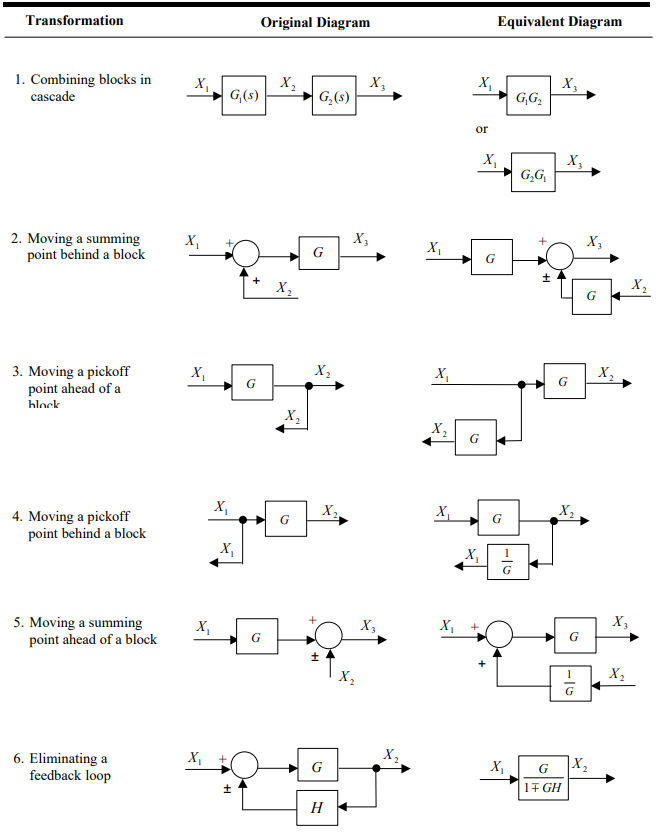
\includegraphics[width=0.7\linewidth]{blockdiagrams.png}
	\label{fig:blockdiagram}
\end{figure}

\newpage
\section{W8: PID Controllers}
\subsection{Automatic Controllers}
\begin{itemize}
    \item Compares actual value of plant/system output with desired value
    \item Controller determines deviation and produces control signal to reduce deviation (control action)
    \item Examples of automatic controllers:
    \begin{itemize}[label=$\circ$]
        \item On-off controllers
        \item PID controllers
        \item Lead-Lag compensators
        \item State Space controllers (30.114)
    \end{itemize}
    \item \textbf{Purpose}: 
    \begin{itemize}[label=$\circ$]
        \item Improve transient response
        \item Enhance steady state performance
        \item Augment or introduce stability into system
    \end{itemize}
\end{itemize}

\subsection{On-off Controllers}
\begin{itemize}
    \item Output depends on value of error between desired and actual values, $e$
    \item Without differential control:
    $$U(t) = \begin{cases}
    \quad U_1, & e>0\\
    \quad U_2, & e<0
    \end{cases}$$
    \begin{center}
        Switch-over point: $e=0$
    \end{center}
    \item With differential control:
    $$U(t) = \begin{cases}
    \quad U_1, & e>e^+\\
    \quad U_2, & e<e^-
    \end{cases}$$
    \begin{center}
        Differential gap: $e^-\leq e \leq e^+$
    \end{center}
    \begin{itemize}[label=$\circ$]
        \item Differential gap allows controller value to maintain value until error has moved significantly from 0 
        \item Tradeoff of accuracy (more switchings) vs operating life
    \end{itemize}
\end{itemize}

\newpage
\subsection{PID Controllers}
\begin{center}
\tikzset{every picture/.style={line width=0.75pt}} %set default line width to 0.75pt        

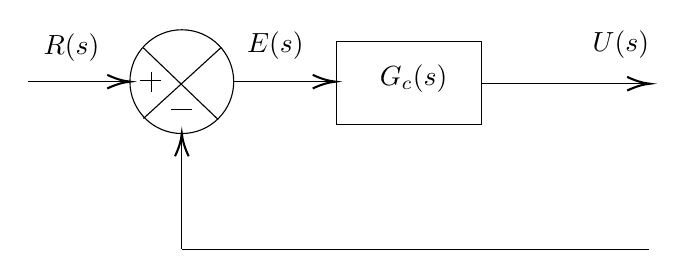
\begin{tikzpicture}[x=0.75pt,y=0.75pt,yscale=-1,xscale=1]
%uncomment if require: \path (0,515); %set diagram left start at 0, and has height of 515

%Shape: Circle [id:dp4181485712735933] 
\draw   (100,149) .. controls (100,135.19) and (111.19,124) .. (125,124) .. controls (138.81,124) and (150,135.19) .. (150,149) .. controls (150,162.81) and (138.81,174) .. (125,174) .. controls (111.19,174) and (100,162.81) .. (100,149) -- cycle ;
%Straight Lines [id:da4740649733052047] 
\draw    (51,149) -- (98,149) ;
\draw [shift={(100,149)}, rotate = 180] [color={rgb, 255:red, 0; green, 0; blue, 0 }  ][line width=0.75]    (10.93,-3.29) .. controls (6.95,-1.4) and (3.31,-0.3) .. (0,0) .. controls (3.31,0.3) and (6.95,1.4) .. (10.93,3.29)   ;
%Straight Lines [id:da3499230348244544] 
\draw    (150,149) -- (197,149) ;
\draw [shift={(199,149)}, rotate = 180] [color={rgb, 255:red, 0; green, 0; blue, 0 }  ][line width=0.75]    (10.93,-3.29) .. controls (6.95,-1.4) and (3.31,-0.3) .. (0,0) .. controls (3.31,0.3) and (6.95,1.4) .. (10.93,3.29)   ;
%Shape: Rectangle [id:dp720053978182877] 
\draw   (199.5,129.5) -- (269.5,129.5) -- (269.5,169.5) -- (199.5,169.5) -- cycle ;
%Straight Lines [id:da444930263203553] 
\draw    (269.5,150) -- (348.5,150) ;
\draw [shift={(350.5,150)}, rotate = 180] [color={rgb, 255:red, 0; green, 0; blue, 0 }  ][line width=0.75]    (10.93,-3.29) .. controls (6.95,-1.4) and (3.31,-0.3) .. (0,0) .. controls (3.31,0.3) and (6.95,1.4) .. (10.93,3.29)   ;
%Straight Lines [id:da11472626901203187] 
% \draw    (321,150.25) -- (321,230.75) ;
%Straight Lines [id:da39388134421732124] 
% \draw    (270.5,230.75) -- (320.5,230.75) ;
%Shape: Rectangle [id:dp21026770917278692] 
% \draw   (200,210.5) -- (270,210.5) -- (270,250.5) -- (200,250.5) -- cycle ;
%Straight Lines [id:da4509078916088618] 
\draw    (125,229.75) -- (350,229.75) ;
%Straight Lines [id:da2451181139005163] 
\draw    (125,229.75) -- (125,176) ;
\draw [shift={(125,174)}, rotate = 450] [color={rgb, 255:red, 0; green, 0; blue, 0 }  ][line width=0.75]    (10.93,-3.29) .. controls (6.95,-1.4) and (3.31,-0.3) .. (0,0) .. controls (3.31,0.3) and (6.95,1.4) .. (10.93,3.29)   ;
%Straight Lines [id:da9337473628239266] 
\draw    (106.5,132.75) -- (142.5,167.25) ;
%Straight Lines [id:da5043252444487525] 
\draw    (144,132.5) -- (106.5,166.75) ;
%Straight Lines [id:da8451547864563302] 
\draw    (105,148.5) -- (115,148.5) ;
%Straight Lines [id:da7484338496828458] 
\draw    (110.5,144.25) -- (110.5,153.75) ;
%Straight Lines [id:da9743377983002497] 
\draw    (120,162.5) -- (130,162.5) ;

% Text Node
\draw (57.14,124.69) node [anchor=north west][inner sep=0.75pt]    {$R( s)$};
% Text Node
\draw (155.14,123.54) node [anchor=north west][inner sep=0.75pt]    {$E( s)$};
% Text Node
\draw (219.14,139.54) node [anchor=north west][inner sep=0.75pt]    {$G_c( s)$};
% Text Node
\draw (321.71,123.26) node [anchor=north west][inner sep=0.75pt]    {$U( s)$};
\end{tikzpicture}
\end{center}
\begin{itemize}
    \item Uses error between desired and actual values to minimize errors by changing controller output
    \item Parameters:
    \begin{itemize}[label=$\circ$]
        \item Proportional: depends on present error\quad $K_pe(t)$
        \item Integral: accumulation of past error\quad $K_i\int_{-\infty}^t e(t)\ dt$
        \item Derivative: prediction of future error\quad$K_d\frac{de(t)}{dt}$
    \end{itemize}
    \item Output in Time Domain: 
    \begin{align*}
        u(t) &= K_pe(t)+K_i\int_{-\infty}^t e(t)+K_d\frac{de(t)}{dt}\\
        &= K_p\left[e(t)+\frac{1}{T_i}\int_{-\infty}^t e(t)\ dt+T_d\displaystyle\frac{de(t)}{dt}\right]
    \end{align*}
    \begin{itemize}[label=$\circ$]
        \item where $K_p$, $K_i$ and $K_d$ are the proportional, integral and derivative gains respectively,
        \item and $T_i$, $T_d$ are the integral and derivative times respectively.
    \end{itemize}
    \item Output in Laplace Domain:
    \begin{align*}
        U(s) &= K_pE(s)+\frac{K_i}{s}E(s)+K_dsE(s)\\
        G_c(s) &= \frac{U(s)}{E(s)}\\
        &= K_p+\frac{K_i}{s}+K_ds\\
        &= K_p\left(1+\frac{1}{T_is}+T_ds\right)
    \end{align*}
\end{itemize}

\subsection{Types of PID Controllers}
\begin{itemize}
    \item P Controller: $$G_c(s) = K_p$$
    \item I Controller:
    \begin{align*}
        G_c(s) &= \frac{K_i}{s}\\
        &= \frac{K_p}{T_is}
    \end{align*}
    \item PI Controller: 
    \begin{align*}
        G_c(s) &= K_p+\frac{K_i}{s}\\
        &= K_p\left(1+\frac{1}{T_is}\right)
    \end{align*}
    \item PD Controller:
    \begin{align*}
        G_c(s) &= K_p+K_ds\\
        &= K_p(1+T_ds)
    \end{align*}
    \item PID Controller: 
    \begin{align*}
        G_c(s) &= K_p+\frac{K_i}{s}+K_ds\\
        &= K_p\left(1+\frac{1}{T_is}+T_ds\right)
    \end{align*}
\end{itemize}

\subsection{Recap: DC Motor}
\begin{itemize}
    \item First order system
    $$G(s) = \frac{A}{Ts+1},\ \text{where }A = \frac{K}{R_ab+KK_b} \text{ and }T=\frac{R_aJ}{R_ab+KK_b}$$
\end{itemize}

\subsection{Proportional Control of First Order System}
\begin{center}
\tikzset{every picture/.style={line width=0.75pt}} %set default line width to 0.75pt
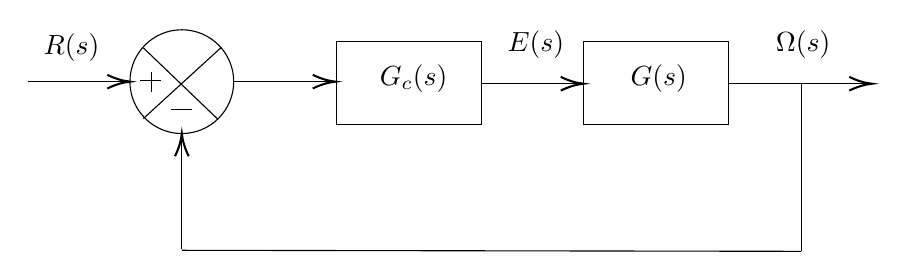
\begin{tikzpicture}[x=0.75pt,y=0.75pt,yscale=-1,xscale=1]
%uncomment if require: \path (0,515); %set diagram left start at 0, and has height of 515

%Shape: Circle [id:dp4181485712735933] 
\draw   (100,149) .. controls (100,135.19) and (111.19,124) .. (125,124) .. controls (138.81,124) and (150,135.19) .. (150,149) .. controls (150,162.81) and (138.81,174) .. (125,174) .. controls (111.19,174) and (100,162.81) .. (100,149) -- cycle ;
%Straight Lines [id:da4740649733052047] 
\draw    (51,149) -- (98,149) ;
\draw [shift={(100,149)}, rotate = 180] [color={rgb, 255:red, 0; green, 0; blue, 0 }  ][line width=0.75]    (10.93,-3.29) .. controls (6.95,-1.4) and (3.31,-0.3) .. (0,0) .. controls (3.31,0.3) and (6.95,1.4) .. (10.93,3.29)   ;
%Straight Lines [id:da3499230348244544] 
\draw    (150,149) -- (197,149) ;
\draw [shift={(199,149)}, rotate = 180] [color={rgb, 255:red, 0; green, 0; blue, 0 }  ][line width=0.75]    (10.93,-3.29) .. controls (6.95,-1.4) and (3.31,-0.3) .. (0,0) .. controls (3.31,0.3) and (6.95,1.4) .. (10.93,3.29)   ;
%Shape: Rectangle [id:dp720053978182877] 
\draw   (199.5,129.5) -- (269.5,129.5) -- (269.5,169.5) -- (199.5,169.5) -- cycle ;
%Straight Lines [id:da444930263203553] 
\draw    (269.5,150) -- (316.5,150) ;
\draw [shift={(318.5,150)}, rotate = 180] [color={rgb, 255:red, 0; green, 0; blue, 0 }  ][line width=0.75]    (10.93,-3.29) .. controls (6.95,-1.4) and (3.31,-0.3) .. (0,0) .. controls (3.31,0.3) and (6.95,1.4) .. (10.93,3.29)   ;
%Shape: Rectangle [id:dp720053978182877] 
\draw   (318.5,129.5) -- (388.5,129.5) -- (388.5,169.5) -- (318.5,169.5) -- cycle ;
%Straight Lines [id:da444930263203553] 
\draw    (388.5,150) -- (455.5,150) ;
\draw [shift={(457.5,150)}, rotate = 180] [color={rgb, 255:red, 0; green, 0; blue, 0 }  ][line width=0.75]    (10.93,-3.29) .. controls (6.95,-1.4) and (3.31,-0.3) .. (0,0) .. controls (3.31,0.3) and (6.95,1.4) .. (10.93,3.29)   ;
%Straight Lines [id:da11472626901203187] 
\draw    (423.5,150.25) -- (423.5,230.75) ;
%Straight Lines [id:da4509078916088618] 
\draw    (125,230.25) -- (423.5,230.75) ;
%Straight Lines [id:da2451181139005163] 
\draw    (125,229.75) -- (125,176) ;
\draw [shift={(125,174)}, rotate = 450] [color={rgb, 255:red, 0; green, 0; blue, 0 }  ][line width=0.75]    (10.93,-3.29) .. controls (6.95,-1.4) and (3.31,-0.3) .. (0,0) .. controls (3.31,0.3) and (6.95,1.4) .. (10.93,3.29)   ;
%Straight Lines [id:da9337473628239266] 
\draw    (106.5,132.75) -- (142.5,167.25) ;
%Straight Lines [id:da5043252444487525] 
\draw    (144,132.5) -- (106.5,166.75) ;
%Straight Lines [id:da8451547864563302] 
\draw    (105,148.5) -- (115,148.5) ;
%Straight Lines [id:da7484338496828458] 
\draw    (110.5,144.25) -- (110.5,153.75) ;
%Straight Lines [id:da9743377983002497] 
\draw    (120,162.5) -- (130,162.5) ;

% Text Node
\draw (57.14,124.69) node [anchor=north west][inner sep=0.75pt]    {$R( s)$};
% Text Node
\draw (219.14,139.54) node [anchor=north west][inner sep=0.75pt]    {$G_c( s)$};
% Text Node
\draw (280.71,123.26) node [anchor=north west][inner sep=0.75pt]    {$E( s)$};
% Text Node
\draw (410,123.26) node [anchor=north west][inner sep=0.75pt]    {$\Omega( s)$};
% Text Node
\draw (340,139.54) node [anchor=north west][inner sep=0.75pt]    {$G( s)$};
\end{tikzpicture}
\end{center}

\begin{itemize}
    \item P Controller: $G_c(s) = K_p$
    \item DC Motor: $G(s) = \displaystyle\frac{A}{Ts+1}$
    \item Closed Loop Transfer Function:
    \begin{align*}
        \frac{\Omega(s)}{R(s)} &= \frac{G_c(s)G(s)}{1+G_c(s)G(s)}= \frac{K_pA}{Ts+1+K_pA}\\
        &= A_p\left(\frac{1}{T_ps+1}\right),\ \text{where }A_p = \frac{K_pA}{1+K_pA}\text{ and }T_p = \frac{T}{1+K_pA}
    \end{align*}
    \begin{itemize}[label=$\circ$]
        \item $A_p$ and $T_p$ are the DC gain and time constants of the closed loop system
        \item $A_p$ and $T_p$ can be changed by adjusting $K_p$
    \end{itemize}
    \item With a unit step input $R(s)$:
    \begin{align*}
        \Omega(s) &= R(s)\frac{A_p}{T_ps+1}\\
        &= \frac{A_p}{s(T_ps+1)}\\
        \Rightarrow \omega(t) &= A_p\left(1-e^{-\frac{t}{T_p}}\right)\\
        &= \frac{K_pA}{1+K_pA}\left(1-e^{-\frac{t}{T_p}}\right)
    \end{align*}
    \item Steady state error, $e_{ss}$:
    \begin{align*}
        e_{ss}&= \lim_{t\to\infty}[r(t)-\omega(t)]\\
        &= 1-\frac{K_pA}{1+K_pA}\\
        &= \frac{1}{1+K_pA}
    \end{align*}
    \begin{itemize}[label=$\circ$]
        \item As $K_p\to\infty$, $e_{ss}\to\infty$.
    \end{itemize}
\end{itemize}

\subsection{Integral Control of First Order System}
\begin{center}
\tikzset{every picture/.style={line width=0.75pt}} %set default line width to 0.75pt        
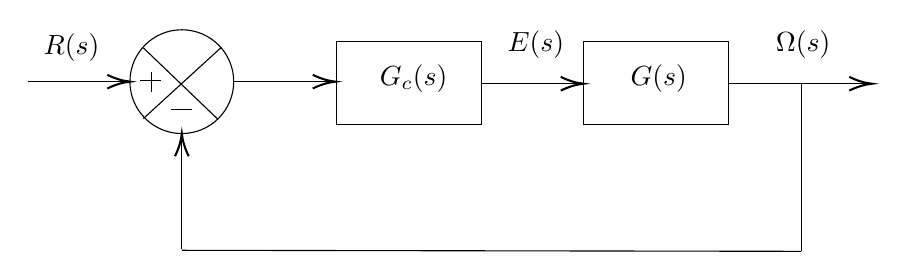
\begin{tikzpicture}[x=0.75pt,y=0.75pt,yscale=-1,xscale=1]
%uncomment if require: \path (0,515); %set diagram left start at 0, and has height of 515

%Shape: Circle [id:dp4181485712735933] 
\draw   (100,149) .. controls (100,135.19) and (111.19,124) .. (125,124) .. controls (138.81,124) and (150,135.19) .. (150,149) .. controls (150,162.81) and (138.81,174) .. (125,174) .. controls (111.19,174) and (100,162.81) .. (100,149) -- cycle ;
%Straight Lines [id:da4740649733052047] 
\draw    (51,149) -- (98,149) ;
\draw [shift={(100,149)}, rotate = 180] [color={rgb, 255:red, 0; green, 0; blue, 0 }  ][line width=0.75]    (10.93,-3.29) .. controls (6.95,-1.4) and (3.31,-0.3) .. (0,0) .. controls (3.31,0.3) and (6.95,1.4) .. (10.93,3.29)   ;
%Straight Lines [id:da3499230348244544] 
\draw    (150,149) -- (197,149) ;
\draw [shift={(199,149)}, rotate = 180] [color={rgb, 255:red, 0; green, 0; blue, 0 }  ][line width=0.75]    (10.93,-3.29) .. controls (6.95,-1.4) and (3.31,-0.3) .. (0,0) .. controls (3.31,0.3) and (6.95,1.4) .. (10.93,3.29)   ;
%Shape: Rectangle [id:dp720053978182877] 
\draw   (199.5,129.5) -- (269.5,129.5) -- (269.5,169.5) -- (199.5,169.5) -- cycle ;
%Straight Lines [id:da444930263203553] 
\draw    (269.5,150) -- (316.5,150) ;
\draw [shift={(318.5,150)}, rotate = 180] [color={rgb, 255:red, 0; green, 0; blue, 0 }  ][line width=0.75]    (10.93,-3.29) .. controls (6.95,-1.4) and (3.31,-0.3) .. (0,0) .. controls (3.31,0.3) and (6.95,1.4) .. (10.93,3.29)   ;
%Shape: Rectangle [id:dp720053978182877] 
\draw   (318.5,129.5) -- (388.5,129.5) -- (388.5,169.5) -- (318.5,169.5) -- cycle ;
%Straight Lines [id:da444930263203553] 
\draw    (388.5,150) -- (455.5,150) ;
\draw [shift={(457.5,150)}, rotate = 180] [color={rgb, 255:red, 0; green, 0; blue, 0 }  ][line width=0.75]    (10.93,-3.29) .. controls (6.95,-1.4) and (3.31,-0.3) .. (0,0) .. controls (3.31,0.3) and (6.95,1.4) .. (10.93,3.29)   ;
%Straight Lines [id:da11472626901203187] 
\draw    (423.5,150.25) -- (423.5,230.75) ;
%Straight Lines [id:da4509078916088618] 
\draw    (125,230.25) -- (423.5,230.75) ;
%Straight Lines [id:da2451181139005163] 
\draw    (125,229.75) -- (125,176) ;
\draw [shift={(125,174)}, rotate = 450] [color={rgb, 255:red, 0; green, 0; blue, 0 }  ][line width=0.75]    (10.93,-3.29) .. controls (6.95,-1.4) and (3.31,-0.3) .. (0,0) .. controls (3.31,0.3) and (6.95,1.4) .. (10.93,3.29)   ;
%Straight Lines [id:da9337473628239266] 
\draw    (106.5,132.75) -- (142.5,167.25) ;
%Straight Lines [id:da5043252444487525] 
\draw    (144,132.5) -- (106.5,166.75) ;
%Straight Lines [id:da8451547864563302] 
\draw    (105,148.5) -- (115,148.5) ;
%Straight Lines [id:da7484338496828458] 
\draw    (110.5,144.25) -- (110.5,153.75) ;
%Straight Lines [id:da9743377983002497] 
\draw    (120,162.5) -- (130,162.5) ;

% Text Node
\draw (57.14,124.69) node [anchor=north west][inner sep=0.75pt]    {$R( s)$};
% Text Node
\draw (219.14,139.54) node [anchor=north west][inner sep=0.75pt]    {$G_c( s)$};
% Text Node
\draw (280.71,123.26) node [anchor=north west][inner sep=0.75pt]    {$E( s)$};
% Text Node
\draw (410,123.26) node [anchor=north west][inner sep=0.75pt]    {$\Omega( s)$};
% Text Node
\draw (340,139.54) node [anchor=north west][inner sep=0.75pt]    {$G( s)$};
\end{tikzpicture}
\end{center}

\begin{itemize}
    \item I Controller: $G_c(s) = \displaystyle\frac{K_i}{s}$
    \item DC Motor: $G(s) = \displaystyle\frac{A}{Ts+1}$
    \item Closed Loop Transfer Function:
    \begin{align*}
        \frac{\Omega(s)}{R(s)}&= \frac{G_c(s)G(s)}{1+G_c(s)G(s)} = \frac{K_iA}{Ts^2+s+K_iA}\\
        &= \frac{\omega_n^2}{s^2+2\zeta\omega_n s+\omega_n^2},\ \text{where }\omega_n^2 = \frac{K_iA}{T}\text{ and }2\zeta\omega_n = \frac{1}{T}
    \end{align*}
    \begin{itemize}[label=$\circ$]
        \item $\omega_n$ can be adjusted by changing $K_i$.
        \item $\zeta$ is indirectly affected by $\omega_n$ and $T$.
    \end{itemize}
    \item Error function $E(s)$:
    \begin{align*}
        \frac{E(s)}{R(s)} &= 1-\frac{\Omega(s)}{R(s)}=1-\frac{\omega_n^2}{s^2+2\zeta\omega_n s+\omega_n^2}\\
        &= \frac{s^2+2\zeta\omega_n s}{s^2+2\zeta\omega_n s+\omega_n^2}\\
        \Rightarrow E(s) &= R(s)\frac{E(s)}{R(s)}\\
        &= \frac{s^2+2\zeta\omega_n s}{s(s^2+2\zeta\omega_n s+\omega_n^2)}
    \end{align*}
    \item Steady state error, $e_{ss}$:
    \begin{align*}
        e_{ss} &= \lim_{s\to 0}sE(s)\\
        &= \lim_{s\to 0}\frac{s^2+2\zeta\omega_n s}{s^2+2\zeta\omega_n s+\omega_n^2}\\
        &= 0
    \end{align*}
    \begin{itemize}[label=$\circ$]
        \item $\therefore$ I controller can remove the steady state error in a first order system.
    \end{itemize}
\end{itemize}

\newpage
\subsection{Proportional Control of Second Order System}
\begin{center}
\tikzset{every picture/.style={line width=0.75pt}} %set default line width to 0.75pt        
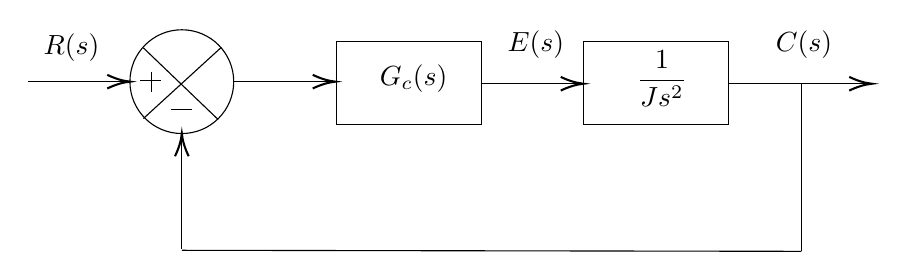
\begin{tikzpicture}[x=0.75pt,y=0.75pt,yscale=-1,xscale=1]
%uncomment if require: \path (0,515); %set diagram left start at 0, and has height of 515

%Shape: Circle [id:dp4181485712735933] 
\draw   (100,149) .. controls (100,135.19) and (111.19,124) .. (125,124) .. controls (138.81,124) and (150,135.19) .. (150,149) .. controls (150,162.81) and (138.81,174) .. (125,174) .. controls (111.19,174) and (100,162.81) .. (100,149) -- cycle ;
%Straight Lines [id:da4740649733052047] 
\draw    (51,149) -- (98,149) ;
\draw [shift={(100,149)}, rotate = 180] [color={rgb, 255:red, 0; green, 0; blue, 0 }  ][line width=0.75]    (10.93,-3.29) .. controls (6.95,-1.4) and (3.31,-0.3) .. (0,0) .. controls (3.31,0.3) and (6.95,1.4) .. (10.93,3.29)   ;
%Straight Lines [id:da3499230348244544] 
\draw    (150,149) -- (197,149) ;
\draw [shift={(199,149)}, rotate = 180] [color={rgb, 255:red, 0; green, 0; blue, 0 }  ][line width=0.75]    (10.93,-3.29) .. controls (6.95,-1.4) and (3.31,-0.3) .. (0,0) .. controls (3.31,0.3) and (6.95,1.4) .. (10.93,3.29)   ;
%Shape: Rectangle [id:dp720053978182877] 
\draw   (199.5,129.5) -- (269.5,129.5) -- (269.5,169.5) -- (199.5,169.5) -- cycle ;
%Straight Lines [id:da444930263203553] 
\draw    (269.5,150) -- (316.5,150) ;
\draw [shift={(318.5,150)}, rotate = 180] [color={rgb, 255:red, 0; green, 0; blue, 0 }  ][line width=0.75]    (10.93,-3.29) .. controls (6.95,-1.4) and (3.31,-0.3) .. (0,0) .. controls (3.31,0.3) and (6.95,1.4) .. (10.93,3.29)   ;
%Shape: Rectangle [id:dp720053978182877] 
\draw   (318.5,129.5) -- (388.5,129.5) -- (388.5,169.5) -- (318.5,169.5) -- cycle ;
%Straight Lines [id:da444930263203553] 
\draw    (388.5,150) -- (455.5,150) ;
\draw [shift={(457.5,150)}, rotate = 180] [color={rgb, 255:red, 0; green, 0; blue, 0 }  ][line width=0.75]    (10.93,-3.29) .. controls (6.95,-1.4) and (3.31,-0.3) .. (0,0) .. controls (3.31,0.3) and (6.95,1.4) .. (10.93,3.29)   ;
%Straight Lines [id:da11472626901203187] 
\draw    (423.5,150.25) -- (423.5,230.75) ;
%Straight Lines [id:da4509078916088618] 
\draw    (125,230.25) -- (423.5,230.75) ;
%Straight Lines [id:da2451181139005163] 
\draw    (125,229.75) -- (125,176) ;
\draw [shift={(125,174)}, rotate = 450] [color={rgb, 255:red, 0; green, 0; blue, 0 }  ][line width=0.75]    (10.93,-3.29) .. controls (6.95,-1.4) and (3.31,-0.3) .. (0,0) .. controls (3.31,0.3) and (6.95,1.4) .. (10.93,3.29)   ;
%Straight Lines [id:da9337473628239266] 
\draw    (106.5,132.75) -- (142.5,167.25) ;
%Straight Lines [id:da5043252444487525] 
\draw    (144,132.5) -- (106.5,166.75) ;
%Straight Lines [id:da8451547864563302] 
\draw    (105,148.5) -- (115,148.5) ;
%Straight Lines [id:da7484338496828458] 
\draw    (110.5,144.25) -- (110.5,153.75) ;
%Straight Lines [id:da9743377983002497] 
\draw    (120,162.5) -- (130,162.5) ;

% Text Node
\draw (57.14,124.69) node [anchor=north west][inner sep=0.75pt]    {$R( s)$};
% Text Node
\draw (219.14,139.54) node [anchor=north west][inner sep=0.75pt]    {$G_c( s)$};
% Text Node
\draw (280.71,123.26) node [anchor=north west][inner sep=0.75pt]    {$E( s)$};
% Text Node
\draw (410,123.26) node [anchor=north west][inner sep=0.75pt]    {$C( s)$};
% Text Node
\draw (343,133) node [anchor=north west][inner sep=0.75pt]    {$\displaystyle\frac{1}{Js^2}$};
\end{tikzpicture}
\end{center}

\begin{itemize}
    \item P Controller: $G_c(s) = K_p$
    \item Second Order System: $G(s) = \displaystyle\frac{1}{Js^2}$
    \item Closed Loop Transfer Function:
    \begin{align*}
        \frac{C(s)}{R(s)} &= \frac{G_c(s)G(s)}{1+G_c(s)G(s)}\\
        &= \frac{K_p}{Js^2+K_p}
    \end{align*}
    \item Characteristic equation: $Js^2+K_p = 0$
    \item Poles: $s=\pm j\sqrt{\displaystyle\frac{K_p}{J}}$
    \begin{itemize}[label=$\circ$]
        \item System oscillates indefinitely
        \item $\therefore$ P controller cannot remove disturbances in a second order system.
    \end{itemize}
\end{itemize}

\subsection{PD Control of Second Order System}
\begin{center}
\tikzset{every picture/.style={line width=0.75pt}} %set default line width to 0.75pt        
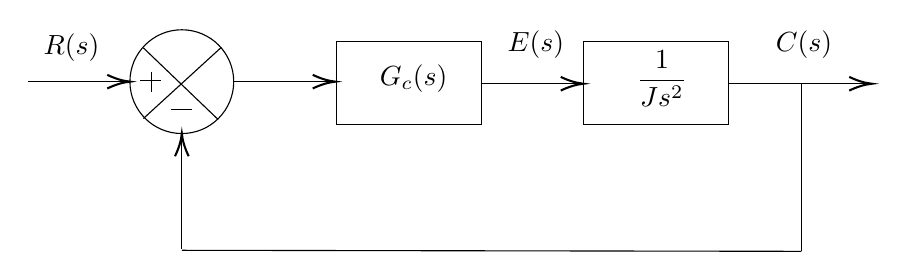
\begin{tikzpicture}[x=0.75pt,y=0.75pt,yscale=-1,xscale=1]
%uncomment if require: \path (0,515); %set diagram left start at 0, and has height of 515

%Shape: Circle [id:dp4181485712735933] 
\draw   (100,149) .. controls (100,135.19) and (111.19,124) .. (125,124) .. controls (138.81,124) and (150,135.19) .. (150,149) .. controls (150,162.81) and (138.81,174) .. (125,174) .. controls (111.19,174) and (100,162.81) .. (100,149) -- cycle ;
%Straight Lines [id:da4740649733052047] 
\draw    (51,149) -- (98,149) ;
\draw [shift={(100,149)}, rotate = 180] [color={rgb, 255:red, 0; green, 0; blue, 0 }  ][line width=0.75]    (10.93,-3.29) .. controls (6.95,-1.4) and (3.31,-0.3) .. (0,0) .. controls (3.31,0.3) and (6.95,1.4) .. (10.93,3.29)   ;
%Straight Lines [id:da3499230348244544] 
\draw    (150,149) -- (197,149) ;
\draw [shift={(199,149)}, rotate = 180] [color={rgb, 255:red, 0; green, 0; blue, 0 }  ][line width=0.75]    (10.93,-3.29) .. controls (6.95,-1.4) and (3.31,-0.3) .. (0,0) .. controls (3.31,0.3) and (6.95,1.4) .. (10.93,3.29)   ;
%Shape: Rectangle [id:dp720053978182877] 
\draw   (199.5,129.5) -- (269.5,129.5) -- (269.5,169.5) -- (199.5,169.5) -- cycle ;
%Straight Lines [id:da444930263203553] 
\draw    (269.5,150) -- (316.5,150) ;
\draw [shift={(318.5,150)}, rotate = 180] [color={rgb, 255:red, 0; green, 0; blue, 0 }  ][line width=0.75]    (10.93,-3.29) .. controls (6.95,-1.4) and (3.31,-0.3) .. (0,0) .. controls (3.31,0.3) and (6.95,1.4) .. (10.93,3.29)   ;
%Shape: Rectangle [id:dp720053978182877] 
\draw   (318.5,129.5) -- (388.5,129.5) -- (388.5,169.5) -- (318.5,169.5) -- cycle ;
%Straight Lines [id:da444930263203553] 
\draw    (388.5,150) -- (455.5,150) ;
\draw [shift={(457.5,150)}, rotate = 180] [color={rgb, 255:red, 0; green, 0; blue, 0 }  ][line width=0.75]    (10.93,-3.29) .. controls (6.95,-1.4) and (3.31,-0.3) .. (0,0) .. controls (3.31,0.3) and (6.95,1.4) .. (10.93,3.29)   ;
%Straight Lines [id:da11472626901203187] 
\draw    (423.5,150.25) -- (423.5,230.75) ;
%Straight Lines [id:da4509078916088618] 
\draw    (125,230.25) -- (423.5,230.75) ;
%Straight Lines [id:da2451181139005163] 
\draw    (125,229.75) -- (125,176) ;
\draw [shift={(125,174)}, rotate = 450] [color={rgb, 255:red, 0; green, 0; blue, 0 }  ][line width=0.75]    (10.93,-3.29) .. controls (6.95,-1.4) and (3.31,-0.3) .. (0,0) .. controls (3.31,0.3) and (6.95,1.4) .. (10.93,3.29)   ;
%Straight Lines [id:da9337473628239266] 
\draw    (106.5,132.75) -- (142.5,167.25) ;
%Straight Lines [id:da5043252444487525] 
\draw    (144,132.5) -- (106.5,166.75) ;
%Straight Lines [id:da8451547864563302] 
\draw    (105,148.5) -- (115,148.5) ;
%Straight Lines [id:da7484338496828458] 
\draw    (110.5,144.25) -- (110.5,153.75) ;
%Straight Lines [id:da9743377983002497] 
\draw    (120,162.5) -- (130,162.5) ;

% Text Node
\draw (57.14,124.69) node [anchor=north west][inner sep=0.75pt]    {$R( s)$};
% Text Node
\draw (219.14,139.54) node [anchor=north west][inner sep=0.75pt]    {$G_c( s)$};
% Text Node
\draw (280.71,123.26) node [anchor=north west][inner sep=0.75pt]    {$E( s)$};
% Text Node
\draw (410,123.26) node [anchor=north west][inner sep=0.75pt]    {$C( s)$};
% Text Node
\draw (343,133) node [anchor=north west][inner sep=0.75pt]    {$\displaystyle\frac{1}{Js^2}$};
\end{tikzpicture}
\end{center}

\begin{itemize}
    \item PD Controller: $G_c(s) = K_p(1+T_ds)$
    \item Second Order System: $G(s) = \frac{1}{Js^2}$
    \item Closed Loop Transfer Function:
    \begin{align*}
        \frac{C(s)}{R(s)} &= \frac{G_c(s)G(s)}{1+G_c(s)G(s)}\\
        &= \frac{K_p(1+T_ds)}{Js^2+K_pT_ds+K_p}
    \end{align*}
    \item Characteristic equation: 
    \begin{align*}
        &Js^2+K_pT_ds+K_p = 0\\
        \Rightarrow\quad &Js^2+K_ds+K_p = 0
    \end{align*}
    \begin{itemize}[label=$\circ$]
        \item Derivative control action introduces damping effect which stabilizes system
    \end{itemize}
\end{itemize}

\subsection{Disturbance Rejection Without Integrator}
\begin{itemize}
    \item Assume a unit step disturbance $D(s)$ is inserted between $G_c(s)$ and $G(s)$.
    \item Let input $R(s) = 0$ and $D(s) = \displaystyle\frac{1}{s}$.
    \item Simplifying the block diagram:
\end{itemize}
\begin{center}
\tikzset{every picture/.style={line width=0.75pt}} %set default line width to 0.75pt
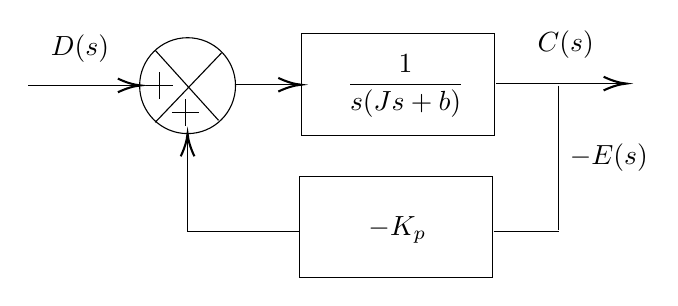
\begin{tikzpicture}[x=0.75pt,y=0.75pt,yscale=-1,xscale=1]
%uncomment if require: \path (0,551); %set diagram left start at 0, and has height of 551
%Straight Lines [id:da7651227515690249] 
\draw    (90.33,192.96) -- (142.46,192.96) ;
\draw [shift={(144.46,192.96)}, rotate = 180] [color={rgb, 255:red, 0; green, 0; blue, 0 }  ][line width=0.75]    (10.93,-3.29) .. controls (6.95,-1.4) and (3.31,-0.3) .. (0,0) .. controls (3.31,0.3) and (6.95,1.4) .. (10.93,3.29)   ;
%Straight Lines [id:da774677464575219] 
\draw    (189.78,192.62) -- (219.75,192.62) ;
\draw [shift={(221.75,192.62)}, rotate = 180] [color={rgb, 255:red, 0; green, 0; blue, 0 }  ][line width=0.75]    (10.93,-3.29) .. controls (6.95,-1.4) and (3.31,-0.3) .. (0,0) .. controls (3.31,0.3) and (6.95,1.4) .. (10.93,3.29)   ;
%Shape: Rectangle [id:dp7571481641218614] 
\draw   (221.99,168.12) -- (315,168.12) -- (315,217.12) -- (221.99,217.12) -- cycle ;
%Straight Lines [id:da1979177245803707] 
\draw    (315.72,192.07) -- (376.5,192.07) ;
\draw [shift={(378.5,192.07)}, rotate = 180] [color={rgb, 255:red, 0; green, 0; blue, 0 }  ][line width=0.75]    (10.93,-3.29) .. controls (6.95,-1.4) and (3.31,-0.3) .. (0,0) .. controls (3.31,0.3) and (6.95,1.4) .. (10.93,3.29)   ;
%Shape: Circle [id:dp35670278384887166] 
\draw   (144,193.07) .. controls (144,180.32) and (154.34,169.97) .. (167.1,169.97) .. controls (179.86,169.97) and (190.2,180.32) .. (190.2,193.07) .. controls (190.2,205.83) and (179.86,216.17) .. (167.1,216.17) .. controls (154.34,216.17) and (144,205.83) .. (144,193.07) -- cycle ;
%Straight Lines [id:da027823258468460343] 
\draw    (151.5,176) -- (182,209.75) ;
%Straight Lines [id:da829089822424002] 
\draw    (183.5,177.25) -- (151.5,210.75) ;
\draw   (147,193) -- (160,193)(153.5,186.5) -- (153.5,199.5) ;
\draw   (159.5,206) -- (172.5,206)(166,199.5) -- (166,212.5) ;
%Shape: Rectangle [id:dp7556162117400378] 
\draw   (220.99,236.62) -- (314,236.62) -- (314,285.62) -- (220.99,285.62) -- cycle ;
%Straight Lines [id:da7051113626481893] 
\draw    (167.1,263.25) -- (167.1,218.17) ;
\draw [shift={(167.1,216.17)}, rotate = 450] [color={rgb, 255:red, 0; green, 0; blue, 0 }  ][line width=0.75]    (10.93,-3.29) .. controls (6.95,-1.4) and (3.31,-0.3) .. (0,0) .. controls (3.31,0.3) and (6.95,1.4) .. (10.93,3.29)   ;
%Straight Lines [id:da5287415827543127] 
\draw    (167,263.25) -- (221.5,263.25) ;
%Straight Lines [id:da467082775598471] 
\draw    (346,193.07) -- (346,262.75) ;
%Straight Lines [id:da5283004348176701] 
\draw    (314.5,263.25) -- (346,263.25) ;
% Text Node
\draw (100,167.13) node [anchor=north west][inner sep=0.75pt]    {$D(s)$};
% Text Node
\draw (242.5,177) node [anchor=north west][inner sep=0.75pt]    {$\displaystyle\frac{1}{s(Js+b)}$};
% Text Node
\draw (253,255) node [anchor=north west][inner sep=0.75pt]    {$-K_p$};
% Text Node
\draw (350,220) node [anchor=north west][inner sep=0.75pt]    {$-E(s)$};
% Text Node
\draw (334.5,165.4) node [anchor=north west][inner sep=0.75pt]    {$C(s)$};
\end{tikzpicture}
\end{center}
\begin{itemize}
    \item Closed Loop Transfer Function:
    \begin{align*}
        \frac{C(s)}{D(s)} &= \frac{\frac{1}{s(Js+b)}}{1+\frac{K_p}{s(Js+b)}}\\
        &= \frac{1}{Js^2+bs+K_p}
    \end{align*}
    \item Error function $E(s)$:
    \begin{align*}
    \frac{E(s)}{D(s)} &= -\frac{C(s)}{D(s)}\\
    &= -\frac{1}{Js^2+bs+K_p}\\
    \Rightarrow E(s) &= -D(s)\frac{C(s)}{D(s)}\\
    &= -\frac{1}{s(Js^2+bs+K_p)}
    \end{align*}
    \item Steady state error, $e_{ss}$:
    \begin{align*}
        e_{ss} &= \lim_{s\to 0}sE(s)\\
        &= -\lim_{s\to 0}\frac{1}{Js^2+bs+K_p}\\
        &= -\frac{1}{K_p}
    \end{align*}
    \begin{itemize}[label=$\circ$]
       \item $\therefore$ P controller cannot remove the steady state error in a first order system.
    \end{itemize}
\end{itemize}

\subsection{Disturbance Rejection With Integrator}
\begin{itemize}
    \item Assume a unit step disturbance $D(s)$ is inserted between $G_c(s)$ and $G(s)$.
    \item Let input $R(s) = 0$ and $D(s) = \displaystyle\frac{1}{s}$.
    \item Simplifying the block diagram:
\end{itemize}
\begin{center}
\tikzset{every picture/.style={line width=0.75pt}} %set default line width to 0.75pt
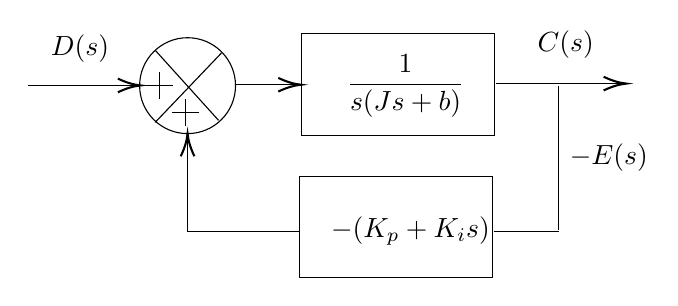
\begin{tikzpicture}[x=0.75pt,y=0.75pt,yscale=-1,xscale=1]
%uncomment if require: \path (0,551); %set diagram left start at 0, and has height of 551
%Straight Lines [id:da7651227515690249] 
\draw    (90.33,192.96) -- (142.46,192.96) ;
\draw [shift={(144.46,192.96)}, rotate = 180] [color={rgb, 255:red, 0; green, 0; blue, 0 }  ][line width=0.75]    (10.93,-3.29) .. controls (6.95,-1.4) and (3.31,-0.3) .. (0,0) .. controls (3.31,0.3) and (6.95,1.4) .. (10.93,3.29)   ;
%Straight Lines [id:da774677464575219] 
\draw    (189.78,192.62) -- (219.75,192.62) ;
\draw [shift={(221.75,192.62)}, rotate = 180] [color={rgb, 255:red, 0; green, 0; blue, 0 }  ][line width=0.75]    (10.93,-3.29) .. controls (6.95,-1.4) and (3.31,-0.3) .. (0,0) .. controls (3.31,0.3) and (6.95,1.4) .. (10.93,3.29)   ;
%Shape: Rectangle [id:dp7571481641218614] 
\draw   (221.99,168.12) -- (315,168.12) -- (315,217.12) -- (221.99,217.12) -- cycle ;
%Straight Lines [id:da1979177245803707] 
\draw    (315.72,192.07) -- (376.5,192.07) ;
\draw [shift={(378.5,192.07)}, rotate = 180] [color={rgb, 255:red, 0; green, 0; blue, 0 }  ][line width=0.75]    (10.93,-3.29) .. controls (6.95,-1.4) and (3.31,-0.3) .. (0,0) .. controls (3.31,0.3) and (6.95,1.4) .. (10.93,3.29)   ;
%Shape: Circle [id:dp35670278384887166] 
\draw   (144,193.07) .. controls (144,180.32) and (154.34,169.97) .. (167.1,169.97) .. controls (179.86,169.97) and (190.2,180.32) .. (190.2,193.07) .. controls (190.2,205.83) and (179.86,216.17) .. (167.1,216.17) .. controls (154.34,216.17) and (144,205.83) .. (144,193.07) -- cycle ;
%Straight Lines [id:da027823258468460343] 
\draw    (151.5,176) -- (182,209.75) ;
%Straight Lines [id:da829089822424002] 
\draw    (183.5,177.25) -- (151.5,210.75) ;
\draw   (147,193) -- (160,193)(153.5,186.5) -- (153.5,199.5) ;
\draw   (159.5,206) -- (172.5,206)(166,199.5) -- (166,212.5) ;
%Shape: Rectangle [id:dp7556162117400378] 
\draw   (220.99,236.62) -- (314,236.62) -- (314,285.62) -- (220.99,285.62) -- cycle ;
%Straight Lines [id:da7051113626481893] 
\draw    (167.1,263.25) -- (167.1,218.17) ;
\draw [shift={(167.1,216.17)}, rotate = 450] [color={rgb, 255:red, 0; green, 0; blue, 0 }  ][line width=0.75]    (10.93,-3.29) .. controls (6.95,-1.4) and (3.31,-0.3) .. (0,0) .. controls (3.31,0.3) and (6.95,1.4) .. (10.93,3.29)   ;
%Straight Lines [id:da5287415827543127] 
\draw    (167,263.25) -- (221.5,263.25) ;
%Straight Lines [id:da467082775598471] 
\draw    (346,193.07) -- (346,262.75) ;
%Straight Lines [id:da5283004348176701] 
\draw    (314.5,263.25) -- (346,263.25) ;
% Text Node
\draw (100,167.13) node [anchor=north west][inner sep=0.75pt]    {$D(s)$};
% Text Node
\draw (242.5,177) node [anchor=north west][inner sep=0.75pt]    {$\displaystyle\frac{1}{s(Js+b)}$};
% Text Node
\draw (235,255) node [anchor=north west][inner sep=0.75pt]    {$-(K_p+K_is)$};
% Text Node
\draw (350,220) node [anchor=north west][inner sep=0.75pt]    {$-E(s)$};
% Text Node
\draw (334.5,165.4) node [anchor=north west][inner sep=0.75pt]    {$C(s)$};
\end{tikzpicture}
\end{center}

\begin{itemize}
    \item Closed Loop Transfer Function:
    \begin{align*}
        \frac{C(s)}{D(s)} &= \frac{\frac{1}{s(Js+b)}}{1+\left(K_p+\frac{K_p}{T_i}\right)\frac{1}{s(Js+b)}}\\
        &= \frac{s}{Js^3+bs^2+K_ps+\frac{K_p}{T_i}}
    \end{align*}
    \item Error function, $E(s)$:
    \begin{align*}
        \frac{E(s)}{D(s)} &= -\frac{C(s)}{D(s)}\\
        &= -\frac{s}{Js^3+bs^2+K_ps+\frac{K_p}{T_i}}\\
        \Rightarrow E(s) &= -D(s)\frac{C(s)}{D(s)}\\
        &= -\frac{s}{s\left(Js^3+bs^2+K_ps+\frac{K_p}{T_i}\right)}
    \end{align*}
    \item Steady state error, $e_{ss}$:
    \begin{align*}
        e_{ss} &= \lim_{s\to 0}sE(s)\\
        &= -\lim_{s\to 0}\frac{s}{Js^3+bs^2+K_ps+\frac{K_p}{T_i}}\\
        &= 0
    \end{align*}
    \begin{itemize}[label=$\circ$]
        \item $\therefore$ PI controller can remove the steady state error in a second order system. 
    \end{itemize}
\end{itemize}

\subsection{PD Controller vs P Controller and Velocity Feedback}
\begin{itemize}
    \item PD Controller

\begin{center}
\tikzset{every picture/.style={line width=0.75pt}} %set default line width to 0.75pt        
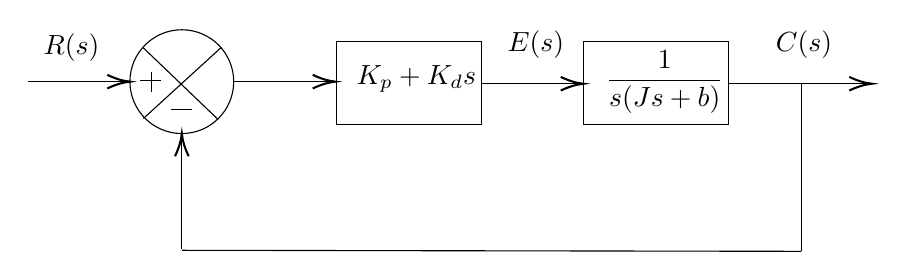
\begin{tikzpicture}[x=0.75pt,y=0.75pt,yscale=-1,xscale=1]
%uncomment if require: \path (0,515); %set diagram left start at 0, and has height of 515
%Shape: Circle [id:dp4181485712735933] 
\draw   (100,149) .. controls (100,135.19) and (111.19,124) .. (125,124) .. controls (138.81,124) and (150,135.19) .. (150,149) .. controls (150,162.81) and (138.81,174) .. (125,174) .. controls (111.19,174) and (100,162.81) .. (100,149) -- cycle ;
%Straight Lines [id:da4740649733052047] 
\draw    (51,149) -- (98,149) ;
\draw [shift={(100,149)}, rotate = 180] [color={rgb, 255:red, 0; green, 0; blue, 0 }  ][line width=0.75]    (10.93,-3.29) .. controls (6.95,-1.4) and (3.31,-0.3) .. (0,0) .. controls (3.31,0.3) and (6.95,1.4) .. (10.93,3.29)   ;
%Straight Lines [id:da3499230348244544] 
\draw    (150,149) -- (197,149) ;
\draw [shift={(199,149)}, rotate = 180] [color={rgb, 255:red, 0; green, 0; blue, 0 }  ][line width=0.75]    (10.93,-3.29) .. controls (6.95,-1.4) and (3.31,-0.3) .. (0,0) .. controls (3.31,0.3) and (6.95,1.4) .. (10.93,3.29)   ;
%Shape: Rectangle [id:dp720053978182877] 
\draw   (199.5,129.5) -- (269.5,129.5) -- (269.5,169.5) -- (199.5,169.5) -- cycle ;
%Straight Lines [id:da444930263203553] 
\draw    (269.5,150) -- (316.5,150) ;
\draw [shift={(318.5,150)}, rotate = 180] [color={rgb, 255:red, 0; green, 0; blue, 0 }  ][line width=0.75]    (10.93,-3.29) .. controls (6.95,-1.4) and (3.31,-0.3) .. (0,0) .. controls (3.31,0.3) and (6.95,1.4) .. (10.93,3.29)   ;
%Shape: Rectangle [id:dp720053978182877] 
\draw   (318.5,129.5) -- (388.5,129.5) -- (388.5,169.5) -- (318.5,169.5) -- cycle ;
%Straight Lines [id:da444930263203553] 
\draw    (388.5,150) -- (455.5,150) ;
\draw [shift={(457.5,150)}, rotate = 180] [color={rgb, 255:red, 0; green, 0; blue, 0 }  ][line width=0.75]    (10.93,-3.29) .. controls (6.95,-1.4) and (3.31,-0.3) .. (0,0) .. controls (3.31,0.3) and (6.95,1.4) .. (10.93,3.29)   ;
%Straight Lines [id:da11472626901203187] 
\draw    (423.5,150.25) -- (423.5,230.75) ;
%Straight Lines [id:da4509078916088618] 
\draw    (125,230.25) -- (423.5,230.75) ;
%Straight Lines [id:da2451181139005163] 
\draw    (125,229.75) -- (125,176) ;
\draw [shift={(125,174)}, rotate = 450] [color={rgb, 255:red, 0; green, 0; blue, 0 }  ][line width=0.75]    (10.93,-3.29) .. controls (6.95,-1.4) and (3.31,-0.3) .. (0,0) .. controls (3.31,0.3) and (6.95,1.4) .. (10.93,3.29)   ;
%Straight Lines [id:da9337473628239266] 
\draw    (106.5,132.75) -- (142.5,167.25) ;
%Straight Lines [id:da5043252444487525] 
\draw    (144,132.5) -- (106.5,166.75) ;
%Straight Lines [id:da8451547864563302] 
\draw    (105,148.5) -- (115,148.5) ;
%Straight Lines [id:da7484338496828458] 
\draw    (110.5,144.25) -- (110.5,153.75) ;
%Straight Lines [id:da9743377983002497] 
\draw    (120,162.5) -- (130,162.5) ;
% Text Node
\draw (57.14,124.69) node [anchor=north west][inner sep=0.75pt]    {$R( s)$};
% Text Node
\draw (208,140) node [anchor=north west][inner sep=0.75pt]    {$K_p+K_ds$};
% Text Node
\draw (280.71,123.26) node [anchor=north west][inner sep=0.75pt]    {$E( s)$};
% Text Node
\draw (410,123.26) node [anchor=north west][inner sep=0.75pt]    {$C( s)$};
% Text Node
\draw (328,133) node [anchor=north west][inner sep=0.75pt]    {$\displaystyle\frac{1}{s(Js+b)}$};
\end{tikzpicture}
\end{center}
\begin{itemize}[label=$\circ$]
    \item Closed Loop Transfer Function:
    \begin{align*}
        \frac{C(s)}{R(s)} &= \frac{\frac{K_p+K_ds}{s(Js+b)}}{1+\frac{K_p+K_ds}{s(Js+b)}}\\
        &= \frac{K_p+K_ds}{Js^2+(b+K_d)s+K_p}
    \end{align*}
    \end{itemize}
\newpage
\item P Controller and Velocity Feedback
\begin{center}
\tikzset{every picture/.style={line width=0.75pt}} %set default line width to 0.75pt        
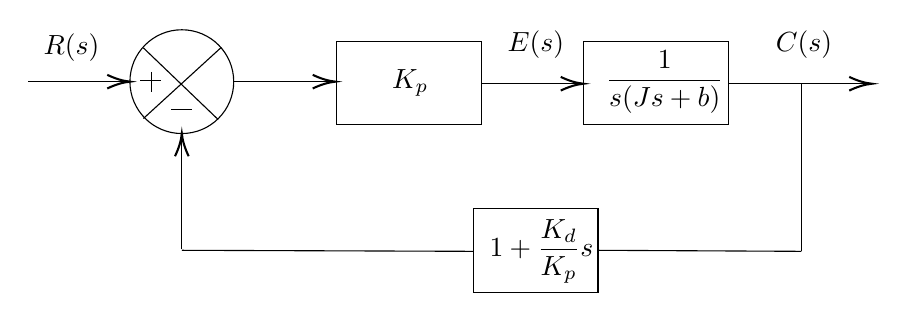
\begin{tikzpicture}[x=0.75pt,y=0.75pt,yscale=-1,xscale=1]
%uncomment if require: \path (0,515); %set diagram left start at 0, and has height of 515
%Shape: Circle [id:dp4181485712735933] 
\draw   (100,149) .. controls (100,135.19) and (111.19,124) .. (125,124) .. controls (138.81,124) and (150,135.19) .. (150,149) .. controls (150,162.81) and (138.81,174) .. (125,174) .. controls (111.19,174) and (100,162.81) .. (100,149) -- cycle ;
%Straight Lines [id:da4740649733052047] 
\draw    (51,149) -- (98,149) ;
\draw [shift={(100,149)}, rotate = 180] [color={rgb, 255:red, 0; green, 0; blue, 0 }  ][line width=0.75]    (10.93,-3.29) .. controls (6.95,-1.4) and (3.31,-0.3) .. (0,0) .. controls (3.31,0.3) and (6.95,1.4) .. (10.93,3.29)   ;
%Straight Lines [id:da3499230348244544] 
\draw    (150,149) -- (197,149) ;
\draw [shift={(199,149)}, rotate = 180] [color={rgb, 255:red, 0; green, 0; blue, 0 }  ][line width=0.75]    (10.93,-3.29) .. controls (6.95,-1.4) and (3.31,-0.3) .. (0,0) .. controls (3.31,0.3) and (6.95,1.4) .. (10.93,3.29)   ;
%Shape: Rectangle [id:dp720053978182877] 
\draw   (199.5,129.5) -- (269.5,129.5) -- (269.5,169.5) -- (199.5,169.5) -- cycle ;
%Straight Lines [id:da444930263203553] 
\draw    (269.5,150) -- (316.5,150) ;
\draw [shift={(318.5,150)}, rotate = 180] [color={rgb, 255:red, 0; green, 0; blue, 0 }  ][line width=0.75]    (10.93,-3.29) .. controls (6.95,-1.4) and (3.31,-0.3) .. (0,0) .. controls (3.31,0.3) and (6.95,1.4) .. (10.93,3.29)   ;
%Shape: Rectangle [id:dp720053978182877] 
\draw   (318.5,129.5) -- (388.5,129.5) -- (388.5,169.5) -- (318.5,169.5) -- cycle ;
%Straight Lines [id:da444930263203553] 
\draw    (388.5,150) -- (455.5,150) ;
\draw [shift={(457.5,150)}, rotate = 180] [color={rgb, 255:red, 0; green, 0; blue, 0 }  ][line width=0.75]    (10.93,-3.29) .. controls (6.95,-1.4) and (3.31,-0.3) .. (0,0) .. controls (3.31,0.3) and (6.95,1.4) .. (10.93,3.29)   ;
%Straight Lines [id:da11472626901203187] 
\draw    (423.5,150.25) -- (423.5,230.75) ;
%Straight Lines [id:da4509078916088618] 
\draw    (125,230.25) -- (265.5,230.75) ;
%Shape: Rectangle [id:dp720053978182877] 
\draw   (265.5,210.25) -- (325.5,210.25) -- (325.5,250.75) -- (265.5,250.75) -- cycle ;
%Straight Lines [id:da4509078916088618] 
\draw    (325.5,230.25) -- (423.5,230.75) ;
%Straight Lines [id:da2451181139005163] 
\draw    (125,229.75) -- (125,176) ;
\draw [shift={(125,174)}, rotate = 450] [color={rgb, 255:red, 0; green, 0; blue, 0 }  ][line width=0.75]    (10.93,-3.29) .. controls (6.95,-1.4) and (3.31,-0.3) .. (0,0) .. controls (3.31,0.3) and (6.95,1.4) .. (10.93,3.29)   ;
%Straight Lines [id:da9337473628239266] 
\draw    (106.5,132.75) -- (142.5,167.25) ;
%Straight Lines [id:da5043252444487525] 
\draw    (144,132.5) -- (106.5,166.75) ;
%Straight Lines [id:da8451547864563302] 
\draw    (105,148.5) -- (115,148.5) ;
%Straight Lines [id:da7484338496828458] 
\draw    (110.5,144.25) -- (110.5,153.75) ;
%Straight Lines [id:da9743377983002497] 
\draw    (120,162.5) -- (130,162.5) ;
% Text Node
\draw (57.14,124.69) node [anchor=north west][inner sep=0.75pt]    {$R( s)$};
% Text Node
\draw (225,142) node [anchor=north west][inner sep=0.75pt]    {$K_p$};
% Text Node
\draw (280.71,123.26) node [anchor=north west][inner sep=0.75pt]    {$E( s)$};
% Text Node
\draw (272,214) node [anchor=north west][inner sep=0.75pt]    {$1+\displaystyle\frac{K_d}{K_p}s$};
% Text Node
\draw (410,123.26) node [anchor=north west][inner sep=0.75pt]    {$C( s)$};
% Text Node
\draw (328,133) node [anchor=north west][inner sep=0.75pt]    {$\displaystyle\frac{1}{s(Js+b)}$};
\end{tikzpicture}
\end{center}
\begin{itemize}[label=$\circ$]
    \item Closed Loop Transfer Function:
    \begin{align*}
        \frac{C(s)}{R(s)} &= \frac{\frac{K_p}{s(Js+b)}}{1+\left(1+\frac{K_d}{K_p}s\right)\frac{K_p}{s(Js+b)}}\\
        &= \frac{K_p}{Js^2+(b+K_d)s+K_p}
    \end{align*}
\end{itemize}
\item Both systems have the same poles but different poles.
\end{itemize}

\subsection{Effect of Zeros on Transient Response}
\begin{itemize}
    \item Zero near a pole
    \begin{itemize}[label=$\circ$]
        \item A zero near a pole reduces that term in overall response
        \begin{align*}
            G_1(s) &= \frac{2}{(s+1)(s+2} = \frac{2}{s+1}-\frac{2}{s+2}\\
            G_2(s) &= \frac{2(s+1.1)}{(s+1)(s+2)} = \frac{\textcolor{red}{0.18}}{s+1}+\frac{1.64}{s+2}
        \end{align*}
    \end{itemize}
    \item Left and right hand plane zeroes
    \begin{itemize}[label=$\circ$]
        \item Consider a second order system $H(s)$:
        \begin{align*}
            H(s) &= \frac{\frac{\omega_n s}{a\zeta}+\omega_n^2}{s^2+2\zeta\omega_n s+\omega_n^2} = \frac{\frac{s}{\alpha\zeta\omega_n}+1}{\frac{s^2}{\omega_n^2}+\frac{2\zeta s}{\omega_n}+1}
        \end{align*}
        \item Let $s = \displaystyle\frac{s}{\omega_n}$:
        \begin{align*}
            \widetilde{H}(s) &= \frac{\frac{s}{\alpha\zeta}+1}{s^2+2\zeta s+1} = \frac{1}{s^2+2\zeta s+1}-\frac{1}{\alpha\zeta}\frac{s}{s^2+2\zeta s+1}\\
            &= H_o(s) + \frac{1}{\alpha\zeta}H_d(s),
        \end{align*}
        \begin{itemize}[label=\tiny$\blacksquare$]
            \item where $H_o$ is the second order system with no zero,
            \item and $H_d$ is the time derivative of $H_o$.
        \end{itemize}
        \item The zero introduces the term $\displaystyle\frac{1}{\alpha\zeta}H_d(s)$.
        \item The second order system has a zero at $s = -\alpha\zeta\omega_n$.
        \begin{itemize}[label=\tiny$\blacksquare$]
            \item If zero is in LHP ($\alpha > 0)$, the system is a minimum phase system.
            \item If zero is in RHP ($\alpha < 0)$, the system is a non-minimum phase system.
            \item More on minimum and non-minimum phase systems in Week 11.
        \end{itemize}
    \end{itemize}
\end{itemize}

\newpage
\subsection{Summary of PID Control Action}
\begin{table}[H]
\centering
\begin{tabular}{|c|c|c|c|c|c|}
\hline
\textbf{Parameter} & \textbf{Rise time, $t_r$} & \textbf{Overshoot, $M_p$} & \textbf{Settling time, $t_s$} & \textbf{Steady state error, $e_{ss}$} & \textbf{System stability}      \\ \hline
$K_p$              & $\downarrow$              & $\uparrow$                & Small $\Delta$                & $\downarrow$                          & $\downarrow$                   \\ \hline
$K_i$              & $\downarrow$              & $\uparrow$                & $\uparrow$                    & Eliminates                            & $\downarrow$                   \\ \hline
$K_d$              & Small $\Delta$            & $\downarrow$              & $\downarrow$                  & No effect                             & $\downarrow$ if $K_d$ is small \\ \hline
\end{tabular}
\end{table}
\begin{itemize}
    \item Proportional Control Action
    \begin{itemize}[label=$\circ$]
        \item Increases speed of response and $\omega_n$
        \item Reduces system stability
    \end{itemize}
    \item Integral Control Action
    \begin{itemize}[label=$\circ$]
        \item Improves steady state performance
        \item Slows down system
        \item Reduces system stability
        \item Increases system order
        \item Rejects disturbances
    \end{itemize}
    \item Derivative Control Action
    \begin{itemize}[label=$\circ$]
        \item Adds damping to system
        \item Improves stability of system
    \end{itemize}
\end{itemize}

\subsection{Tuning PID Controllers}
\begin{itemize}
    \item Heuristic method formulated in by Ziegler and Nichols in 1942
    \item Ziegler-Nicholas Tuning has 2 methods:
    \begin{itemize}[label=$\circ$]
        \item Open loop tuning method
        \item Closed loop tuning method
    \end{itemize}
    \item Gives educated guess for controller gains
    \item Provides good starting point for further fine tuning
\end{itemize}

\newpage
\subsection{Open Loop Ziegler-Nicholas Tuning}
\begin{itemize}
    \item Draw a tangent line at the inflection point of the open loop unit step output:

\begin{center}
\tikzset{every picture/.style={line width=0.75pt}} %set default line width to 0.75p
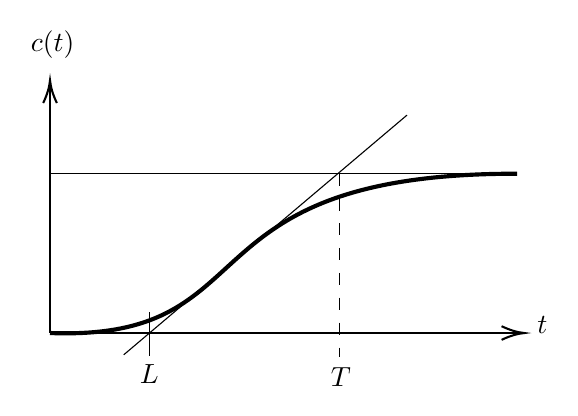
\begin{tikzpicture}[x=0.75pt,y=0.75pt,yscale=-1,xscale=1]
%Straight Lines [id:da04698426886111373] 
\draw    (100,189.75) -- (100,70) ;
\draw [shift={(100,68)}, rotate = 450] [color={rgb, 255:red, 0; green, 0; blue, 0 }  ][line width=0.75]    (10.93,-3.29) .. controls (6.95,-1.4) and (3.31,-0.3) .. (0,0) .. controls (3.31,0.3) and (6.95,1.4) .. (10.93,3.29)   ;
%Straight Lines [id:da8402673974183574] 
\draw    (100,189.75) -- (326.5,189.75) ;
\draw [shift={(328.5,189.75)}, rotate = 180] [color={rgb, 255:red, 0; green, 0; blue, 0 }  ][line width=0.75]    (10.93,-3.29) .. controls (6.95,-1.4) and (3.31,-0.3) .. (0,0) .. controls (3.31,0.3) and (6.95,1.4) .. (10.93,3.29)   ;
%Straight Lines [id:da05421989901691604] 
\draw    (100,113) -- (325,113) ;
%Curve Lines [id:da7197149735120874] 
\draw [line width=1.5]    (100,189.75) .. controls (207.5,193.75) and (160.5,112.75) .. (325,113) ;
%Straight Lines [id:da9511781654944775] 
\draw    (272,84.75) -- (135.5,200.25) ;
%Straight Lines [id:da44638051513655985] 
\draw  [dash pattern={on 4.5pt off 4.5pt}]  (239.5,112.75) -- (239.5,201.25) ;
%Straight Lines [id:da6185848066098356] 
\draw    (148,179.75) -- (148,200.75) ;
% Text Node
\draw (333.5,180.4) node [anchor=north west][inner sep=0.75pt]    {$t$};
% Text Node
\draw (89.5,42.9) node [anchor=north west][inner sep=0.75pt]    {$c( t)$};
% Text Node
\draw (234,204.9) node [anchor=north west][inner sep=0.75pt]    {$T$};
% Text Node
\draw (142,203.9) node [anchor=north west][inner sep=0.75pt]    {$L$};
\end{tikzpicture}
\end{center}
\item Comprises 2 experimental parameters:
\begin{itemize}[label=$\circ$]
    \item Lag time, $L$: where the tangent line cuts the time axis
    \item Approximated time constant, $T$: where the tangent line cuts the steady state response
\end{itemize}
\item Recommended PID controller gains:
\begin{table}[H]
\centering\makegapedcells
\begin{tabular}{|c|c|c|c|}
\hline
\textbf{\begin{tabular}[c]{@{}c@{}}Type of \\ Controller\end{tabular}} & \textbf{\begin{tabular}[c]{@{}c@{}}Proportional gain,\\ $K_p$\end{tabular}} & \textbf{\begin{tabular}[c]{@{}c@{}}Integral time,\\ $T_i$\end{tabular}} & \textbf{\begin{tabular}[c]{@{}c@{}}Differential time,\\ $T_d$\end{tabular}} \\ \hline
P                                                                      & $\displaystyle\frac{T}{L}$                                                  & -                                              & -                                                   \\ \hline
PI                                                                     & $0.9\displaystyle\frac{T}{L}$                                               & $\displaystyle\frac{L}{0.3}$                                            & -                                              \\ \hline
PID                                                                    & $1.2\displaystyle\frac{T}{L}$                                               & $2L$                                                                    & $0.5L$                                                                      \\ \hline
\end{tabular}
\end{table}
\end{itemize}

\subsection{Closed Loop Ziegler-Nicholas Tuning}
\begin{itemize}
    \item With only the P controller, increase $K_p$ until the output shows sustained oscillations.
    \item $K_p$ at this point is known as the critical value $K_{cr}$.
    \item The corresponding period $P_{cr}$ can also be found.
    \item Recommended PID controller gains:
    \begin{table}[H]
    \centering\makegapedcells
\begin{tabular}{|c|c|c|c|}
\hline
\textbf{\begin{tabular}[c]{@{}c@{}}Type of \\ Controller\end{tabular}} & \textbf{\begin{tabular}[c]{@{}c@{}}Proportional gain,\\ $K_p$\end{tabular}} & \textbf{\begin{tabular}[c]{@{}c@{}}Integral time,\\ $T_i$\end{tabular}} & \textbf{\begin{tabular}[c]{@{}c@{}}Differential time,\\ $T_d$\end{tabular}} \\ \hline
P                                                                      & $0.5K_{cr}$                                                                 & -  &                      -                          \\ \hline
PI                                                                     & $0.45K_{cr}$                                                                & $\displaystyle\frac{P_{cr}}{1.2}$                                       & -                                                  \\ \hline
PID                                                                    & $0.6K_{cr}$                                                                 & $0.5P_{cr}$                                                             & $0.125P_{cr}$                                                               \\ \hline
\end{tabular}
\end{table}
\end{itemize}

\section{W10: Linearization}
\subsection{Purpose of Linearization}
\begin{itemize}
    \item Allows linear analysis methods to be used on non-linear systems
    \item e.g. small angle approximation $\sin\theta \approx \theta$
\end{itemize}

\subsection{Linearization about a Point (x, z)}
\begin{itemize}
    \item Choose an operating point $(\Bar{x},\ \Bar{z})$.
    \item If $x-\Bar{x}$ is small and $\Bar{z} = f(\Bar{x})$, ignoring the higher order terms:
    \begin{align*}
        z-\Bar{z} &= \left.\frac{df(x)}{dx}\right|_{x = \Bar{x}}(x-\Bar{x})\\
        \Rightarrow \hat{z} &= \left.\frac{df(x)}{dx}\right|_{x = \Bar{x}}\hat{x}
    \end{align*}
    \begin{itemize}[label=$\circ$]
        \item where $\hat{x} = x-\Bar{x}$ and $\hat{z} = z-\Bar{z}$.
    \end{itemize}
\end{itemize}

\subsection{Linearization about a Point (x, y, z)}
\begin{itemize}
    \item Choose an operating point $(\Bar{x},\ \Bar{y},\ \Bar{z})$.
    \item If $x-\Bar{x}$ and $y-\Bar{y}$ are small and $\Bar{z} = f(\Bar{x},\ \Bar{y})$, ignoring the higher order terms:
    \begin{align*}
        z-\Bar{z} &= \left.\frac{\partial f(x,\ y)}{\partial x}\right|_{\substack{x = \Bar{x}\\ y= \Bar{y}}} (x-\Bar{x})+\left.\frac{\partial f(x,\ y)}{\partial y}\right|_{\substack{x = \Bar{x}\\ y= \Bar{y}}} (y-\Bar{y})\\
        \Rightarrow \hat{z} &= \left.\frac{\partial f(x,\ y)}{\partial x}\right|_{\substack{x = \Bar{x}\\ y= \Bar{y}}}\hat{x}+\left.\frac{\partial f(x,\ y)}{\partial y}\right|_{\substack{x = \Bar{x}\\ y= \Bar{y}}}\hat{y}
    \end{align*}
    \begin{itemize}[label=$\circ$]
        \item where $\hat{x} = x-\Bar{x}$, $\hat{y} = y-\Bar{y}$ and $\hat{z} = z-\Bar{z}$.
    \end{itemize}
\end{itemize}

\newpage
\section{W10: System Stability}
\subsection{Stability Analysis}
\begin{itemize}
    \item Stability is a critical concern.
    \item Stability is a system property, does not depend on inputs.
    \item Types of stability:
    \begin{itemize}[label=$\circ$]
        \item Absolute/ internal stability: LHP poles
        \item Neutral stability: Non-repeated $j\omega$ axis poles
        \item Unstable: Repeated $j\omega$ axis poles, RHP poles
    \end{itemize}
\end{itemize}

\subsection{Routh-Hurwitz Stability Criterion}
\begin{enumerate}
    \item Write characteristic equation in descending powers of $s$.
    \item If coefficients contain zero or negative values, there are imaginary poles or RHP poles.\\
    $\Rightarrow$ System is not stable.
    \item If coefficients are positive, construct a Routh Array.
    \item No. of RHP poles in CE = no. of changes in sign of coefficients in 1st column of Routh array
\end{enumerate}

e.g. $s^4+2s^3+3s^2+4s+5=0$\\
\begin{minipage}{0.3\textwidth}
\begin{table}[H]
\begin{tabular}{cccc}
$s^4$ & $a_1 = 1$ & $a_2 = 3$ & $a_3 = 5$ \\
$s^3$ & $b_1 = 2$ & $b_2 = 4$ &           \\
$s^2$ & $c_1$     & $c_2$     &           \\
$s^1$ & $d_1$     &           &           \\
$s^0$ & $e_1$     &           &          
\end{tabular}
\end{table}
\end{minipage}
\begin{minipage}{0.7\textwidth}
\begin{align*}
    c_1 &= \frac{b_1a_2-a_1b_2}{b_1}= 1,\quad c_2 = \frac{b_2a_3-0}{b_2}=5\\
    d_1 &= \frac{c_1b_2-b_1c_2}{c_1} = -6\\
    e_1 &= \frac{d_1c_2-0}{d_1} = 5
\end{align*}
\end{minipage}
\mbox{}\\
There are 2 sign changes and thus 2 RHP poles, $\therefore$ the system is unstable.

\subsection{Special Cases of Routh Array}
\subsubsection{Zero in First Column}
e.g. $s^3+2s^2+s+2=0$\\
\begin{minipage}{0.2\textwidth}
\begin{table}[H]
\begin{tabular}{ccc}
$s^3$ & 1                  & 1 \\
$s^2$ & 2                  & 2 \\
$s^1$ & $0\approx\epsilon$ &   \\
$s^0$ & 2                  &  
\end{tabular}
\end{table}
\end{minipage}
\begin{minipage}{0.8\textwidth}
\begin{itemize}
    \item Replace zero with a small positive number, $\epsilon$.
    \item Indicates presence of a pair of imaginary roots.
\end{itemize}
\end{minipage}

\subsubsection{Zeros in Entire Derived Row}
e.g. $s^5+2s^4+24s^3+48s^2-25s-50=0$\\
\begin{minipage}{0.25\textwidth}
\begin{table}[H]
\begin{tabular}{cccc}
$s^5$ & 1           & 24           & -25 \\
$s^4$ & 2           & 48           & -50 \\
$s^3$ & \cancel{0} 8 & \cancel{0} 96 &     \\
$s^2$ & 24          & -50          &     \\
$s^1$ & 112.7       &              &     \\
$s^0$ & -50         &              &    
\end{tabular}
\end{table}
\end{minipage}
\begin{minipage}{0.75\textwidth}
\begin{itemize}
    \item Create an auxiliary polynomial $P(s)$ from row above. \item Replace the coefficients of the zero row with $\displaystyle\frac{dP(s)}{ds}$:
    \begin{center}
        \boxed{
        \begin{array}{ccc}
            P(s) &=& 2s^4+48s^2-50\\
            \Rightarrow \frac{dP(s)}{ds} &=& 8s^3+96s
        \end{array}}
    \end{center}
    \item Denotes presence of radially opposite poles in $s$-plane.
\end{itemize}
\end{minipage}

\newpage
\section{W10: System Types}
\begin{center}
\tikzset{every picture/.style={line width=0.75pt}} %set default line width to 0.75pt        
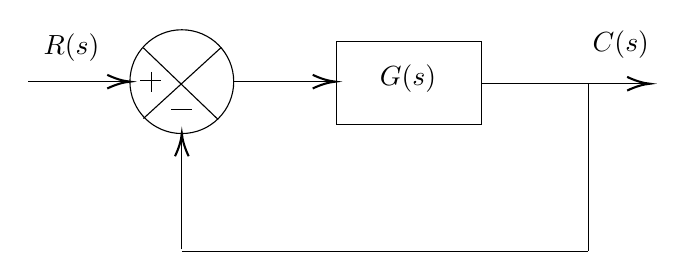
\begin{tikzpicture}[x=0.75pt,y=0.75pt,yscale=-1,xscale=1]
%uncomment if require: \path (0,515); %set diagram left start at 0, and has height of 515
%Shape: Circle [id:dp4181485712735933] 
\draw   (100,149) .. controls (100,135.19) and (111.19,124) .. (125,124) .. controls (138.81,124) and (150,135.19) .. (150,149) .. controls (150,162.81) and (138.81,174) .. (125,174) .. controls (111.19,174) and (100,162.81) .. (100,149) -- cycle ;
%Straight Lines [id:da4740649733052047] 
\draw    (51,149) -- (98,149) ;
\draw [shift={(100,149)}, rotate = 180] [color={rgb, 255:red, 0; green, 0; blue, 0 }  ][line width=0.75]    (10.93,-3.29) .. controls (6.95,-1.4) and (3.31,-0.3) .. (0,0) .. controls (3.31,0.3) and (6.95,1.4) .. (10.93,3.29)   ;
%Straight Lines [id:da3499230348244544] 
\draw    (150,149) -- (197,149) ;
\draw [shift={(199,149)}, rotate = 180] [color={rgb, 255:red, 0; green, 0; blue, 0 }  ][line width=0.75]    (10.93,-3.29) .. controls (6.95,-1.4) and (3.31,-0.3) .. (0,0) .. controls (3.31,0.3) and (6.95,1.4) .. (10.93,3.29)   ;
%Shape: Rectangle [id:dp720053978182877] 
\draw   (199.5,129.5) -- (269.5,129.5) -- (269.5,169.5) -- (199.5,169.5) -- cycle ;
%Straight Lines [id:da444930263203553] 
\draw    (269.5,150) -- (348.5,150) ;
\draw [shift={(350.5,150)}, rotate = 180] [color={rgb, 255:red, 0; green, 0; blue, 0 }  ][line width=0.75]    (10.93,-3.29) .. controls (6.95,-1.4) and (3.31,-0.3) .. (0,0) .. controls (3.31,0.3) and (6.95,1.4) .. (10.93,3.29)   ;
%Straight Lines [id:da11472626901203187] 
\draw    (321,150.25) -- (321,230.75) ;
%Straight Lines [id:da4509078916088618] 
\draw    (125,230.75) -- (320.5,230.75) ;
%Straight Lines [id:da2451181139005163] 
\draw    (125,229.75) -- (125,176) ;
\draw [shift={(125,174)}, rotate = 450] [color={rgb, 255:red, 0; green, 0; blue, 0 }  ][line width=0.75]    (10.93,-3.29) .. controls (6.95,-1.4) and (3.31,-0.3) .. (0,0) .. controls (3.31,0.3) and (6.95,1.4) .. (10.93,3.29)   ;
%Straight Lines [id:da9337473628239266] 
\draw    (106.5,132.75) -- (142.5,167.25) ;
%Straight Lines [id:da5043252444487525] 
\draw    (144,132.5) -- (106.5,166.75) ;
%Straight Lines [id:da8451547864563302] 
\draw    (105,148.5) -- (115,148.5) ;
%Straight Lines [id:da7484338496828458] 
\draw    (110.5,144.25) -- (110.5,153.75) ;
%Straight Lines [id:da9743377983002497] 
\draw    (120,162.5) -- (130,162.5) ;
% Text Node
\draw (57.14,124.69) node [anchor=north west][inner sep=0.75pt]    {$R( s)$};
% Text Node
\draw (219.14,139.54) node [anchor=north west][inner sep=0.75pt]    {$G( s)$};
% Text Node
\draw (321.71,123.26) node [anchor=north west][inner sep=0.75pt]    {$C( s)$};
\end{tikzpicture}
\end{center}

\begin{itemize}
    \item Consider under unity feedback $H(s) = 1$
    $$G(s) = K\frac{(\tau_1s+1)(\tau_2s+1)\cdots(\tau_ms+1)}{s^N(T_1s+1)(T_2s+1)\cdots(T_ns+1)}$$
    \begin{itemize}[label=$\circ$]
        \item System Order: $N+n$
        \item No. of poles: $N+n$
    \end{itemize}
    \item System is classified by pole multiplicity $N$ at the origin:
    \begin{align*}
        N = 0 & \Rightarrow \text{Type 0 system}\\
        N = 1 & \Rightarrow \text{Type 1 system}\\
        N = 2 & \Rightarrow \text{Type 2 system}
    \end{align*}
    \begin{itemize}[label=$\circ$]
        \item \textcolor{red}{System Order $\neq$ System Type}
    \end{itemize}
\end{itemize}

\subsection{Static Position Error Constant}
\begin{center}
\tikzset{every picture/.style={line width=0.75pt}} %set default line width to 0.75pt        
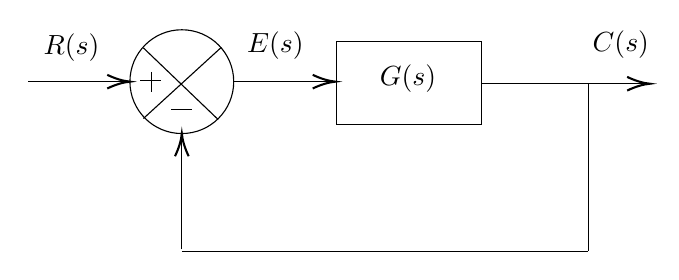
\begin{tikzpicture}[x=0.75pt,y=0.75pt,yscale=-1,xscale=1]
%uncomment if require: \path (0,515); %set diagram left start at 0, and has height of 515
%Shape: Circle [id:dp4181485712735933] 
\draw   (100,149) .. controls (100,135.19) and (111.19,124) .. (125,124) .. controls (138.81,124) and (150,135.19) .. (150,149) .. controls (150,162.81) and (138.81,174) .. (125,174) .. controls (111.19,174) and (100,162.81) .. (100,149) -- cycle ;
%Straight Lines [id:da4740649733052047] 
\draw    (51,149) -- (98,149) ;
\draw [shift={(100,149)}, rotate = 180] [color={rgb, 255:red, 0; green, 0; blue, 0 }  ][line width=0.75]    (10.93,-3.29) .. controls (6.95,-1.4) and (3.31,-0.3) .. (0,0) .. controls (3.31,0.3) and (6.95,1.4) .. (10.93,3.29)   ;
%Straight Lines [id:da3499230348244544] 
\draw    (150,149) -- (197,149) ;
\draw [shift={(199,149)}, rotate = 180] [color={rgb, 255:red, 0; green, 0; blue, 0 }  ][line width=0.75]    (10.93,-3.29) .. controls (6.95,-1.4) and (3.31,-0.3) .. (0,0) .. controls (3.31,0.3) and (6.95,1.4) .. (10.93,3.29)   ;
%Shape: Rectangle [id:dp720053978182877] 
\draw   (199.5,129.5) -- (269.5,129.5) -- (269.5,169.5) -- (199.5,169.5) -- cycle ;
%Straight Lines [id:da444930263203553] 
\draw    (269.5,150) -- (348.5,150) ;
\draw [shift={(350.5,150)}, rotate = 180] [color={rgb, 255:red, 0; green, 0; blue, 0 }  ][line width=0.75]    (10.93,-3.29) .. controls (6.95,-1.4) and (3.31,-0.3) .. (0,0) .. controls (3.31,0.3) and (6.95,1.4) .. (10.93,3.29)   ;
%Straight Lines [id:da11472626901203187] 
\draw    (321,150.25) -- (321,230.75) ;
%Straight Lines [id:da4509078916088618] 
\draw    (125,230.75) -- (320.5,230.75) ;
%Straight Lines [id:da2451181139005163] 
\draw    (125,229.75) -- (125,176) ;
\draw [shift={(125,174)}, rotate = 450] [color={rgb, 255:red, 0; green, 0; blue, 0 }  ][line width=0.75]    (10.93,-3.29) .. controls (6.95,-1.4) and (3.31,-0.3) .. (0,0) .. controls (3.31,0.3) and (6.95,1.4) .. (10.93,3.29)   ;
%Straight Lines [id:da9337473628239266] 
\draw    (106.5,132.75) -- (142.5,167.25) ;
%Straight Lines [id:da5043252444487525] 
\draw    (144,132.5) -- (106.5,166.75) ;
%Straight Lines [id:da8451547864563302] 
\draw    (105,148.5) -- (115,148.5) ;
%Straight Lines [id:da7484338496828458] 
\draw    (110.5,144.25) -- (110.5,153.75) ;
%Straight Lines [id:da9743377983002497] 
\draw    (120,162.5) -- (130,162.5) ;
% Text Node
\draw (57.14,124.69) node [anchor=north west][inner sep=0.75pt]    {$R( s)$};
% Text Node
\draw (219.14,139.54) node [anchor=north west][inner sep=0.75pt]    {$G( s)$};
% Text Node
\draw (321.71,123.26) node [anchor=north west][inner sep=0.75pt]    {$C( s)$};
% Text Node
\draw (155.14,123.54) node [anchor=north west][inner sep=0.75pt]    {$E( s)$};
\end{tikzpicture}
\end{center}

\begin{itemize}
    \item R(s) is a unit step input, $\therefore R(s) = \displaystyle\frac{1}{s}$
    \item Closed Loop Transfer Function:
    \begin{align*}
        \frac{C(s)}{R(s)} &= \frac{G(s)}{1+G(s)}
    \end{align*}
    \item Error function, $E(s)$:
    \begin{align*}
        \frac{E(s)}{R(s)} &= 1-\frac{C(s)}{R(s)} = \frac{1}{1+G(s)}\\
        E(s) &= R(s)\frac{E(s)}{R(s)} = \frac{1}{s(1+G(s))}
    \end{align*}
    \item Steady state error, $e_{ss}$:
    \begin{align*}
        e_{ss} &= \lim_{s\to 0}sE(s)\\
        &= \lim_{s\to 0}\frac{1}{1+G(s)}\\
        &= \frac{1}{1+K_P}
    \end{align*}
    \item Static Position Error Constant, $K_P$:
    $$K_P = \lim_{s\to 0}G(s)$$
\end{itemize}

\subsection{Static Velocity Error Constant}
\begin{center}
\tikzset{every picture/.style={line width=0.75pt}} %set default line width to 0.75pt        
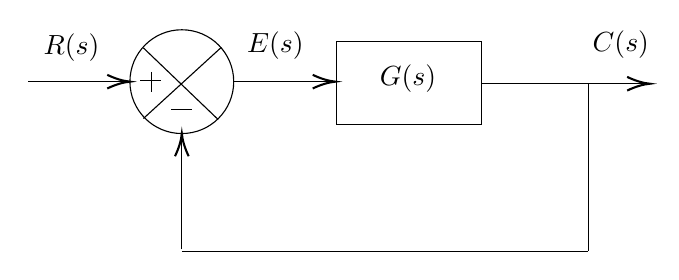
\begin{tikzpicture}[x=0.75pt,y=0.75pt,yscale=-1,xscale=1]
%uncomment if require: \path (0,515); %set diagram left start at 0, and has height of 515
%Shape: Circle [id:dp4181485712735933] 
\draw   (100,149) .. controls (100,135.19) and (111.19,124) .. (125,124) .. controls (138.81,124) and (150,135.19) .. (150,149) .. controls (150,162.81) and (138.81,174) .. (125,174) .. controls (111.19,174) and (100,162.81) .. (100,149) -- cycle ;
%Straight Lines [id:da4740649733052047] 
\draw    (51,149) -- (98,149) ;
\draw [shift={(100,149)}, rotate = 180] [color={rgb, 255:red, 0; green, 0; blue, 0 }  ][line width=0.75]    (10.93,-3.29) .. controls (6.95,-1.4) and (3.31,-0.3) .. (0,0) .. controls (3.31,0.3) and (6.95,1.4) .. (10.93,3.29)   ;
%Straight Lines [id:da3499230348244544] 
\draw    (150,149) -- (197,149) ;
\draw [shift={(199,149)}, rotate = 180] [color={rgb, 255:red, 0; green, 0; blue, 0 }  ][line width=0.75]    (10.93,-3.29) .. controls (6.95,-1.4) and (3.31,-0.3) .. (0,0) .. controls (3.31,0.3) and (6.95,1.4) .. (10.93,3.29)   ;
%Shape: Rectangle [id:dp720053978182877] 
\draw   (199.5,129.5) -- (269.5,129.5) -- (269.5,169.5) -- (199.5,169.5) -- cycle ;
%Straight Lines [id:da444930263203553] 
\draw    (269.5,150) -- (348.5,150) ;
\draw [shift={(350.5,150)}, rotate = 180] [color={rgb, 255:red, 0; green, 0; blue, 0 }  ][line width=0.75]    (10.93,-3.29) .. controls (6.95,-1.4) and (3.31,-0.3) .. (0,0) .. controls (3.31,0.3) and (6.95,1.4) .. (10.93,3.29)   ;
%Straight Lines [id:da11472626901203187] 
\draw    (321,150.25) -- (321,230.75) ;
%Straight Lines [id:da4509078916088618] 
\draw    (125,230.75) -- (320.5,230.75) ;
%Straight Lines [id:da2451181139005163] 
\draw    (125,229.75) -- (125,176) ;
\draw [shift={(125,174)}, rotate = 450] [color={rgb, 255:red, 0; green, 0; blue, 0 }  ][line width=0.75]    (10.93,-3.29) .. controls (6.95,-1.4) and (3.31,-0.3) .. (0,0) .. controls (3.31,0.3) and (6.95,1.4) .. (10.93,3.29)   ;
%Straight Lines [id:da9337473628239266] 
\draw    (106.5,132.75) -- (142.5,167.25) ;
%Straight Lines [id:da5043252444487525] 
\draw    (144,132.5) -- (106.5,166.75) ;
%Straight Lines [id:da8451547864563302] 
\draw    (105,148.5) -- (115,148.5) ;
%Straight Lines [id:da7484338496828458] 
\draw    (110.5,144.25) -- (110.5,153.75) ;
%Straight Lines [id:da9743377983002497] 
\draw    (120,162.5) -- (130,162.5) ;
% Text Node
\draw (57.14,124.69) node [anchor=north west][inner sep=0.75pt]    {$R( s)$};
% Text Node
\draw (219.14,139.54) node [anchor=north west][inner sep=0.75pt]    {$G( s)$};
% Text Node
\draw (321.71,123.26) node [anchor=north west][inner sep=0.75pt]    {$C( s)$};
% Text Node
\draw (155.14,123.54) node [anchor=north west][inner sep=0.75pt]    {$E( s)$};
\end{tikzpicture}
\end{center}

\begin{itemize}
    \item R(s) is a unit ramp input, $\therefore R(s) = \displaystyle\frac{1}{s^2}$
    \item Closed Loop Transfer Function:
    $$\frac{C(s)}{R(s)} = \frac{G(s)}{1+G(s)}$$
    \item Error function, $E(s)$:
    \begin{align*}
        \frac{E(s)}{R(s)} &= 1-\frac{C(s)}{R(s)} = \frac{1}{1+G(s)}\\
        E(s) &= R(s)\frac{E(s)}{R(s)} = \frac{1}{s^2(1+G(s))}
    \end{align*}
    \item Steady state error, $e_{ss}$:
    \begin{align*}
        e_{ss} &= \lim_{s\to 0}sE(s)\\
        &= \lim_{s\to 0}\frac{1}{s(1+G(s))}\\
        &= \frac{1}{K_V}
    \end{align*}
    \item Static Velocity Error Constant, $K_V$:
    $$K_V = \lim_{s\to 0}sG(s)$$
\end{itemize}

\subsection{Static Acceleration Error Constant}
\begin{center}
\tikzset{every picture/.style={line width=0.75pt}} %set default line width to 0.75pt        
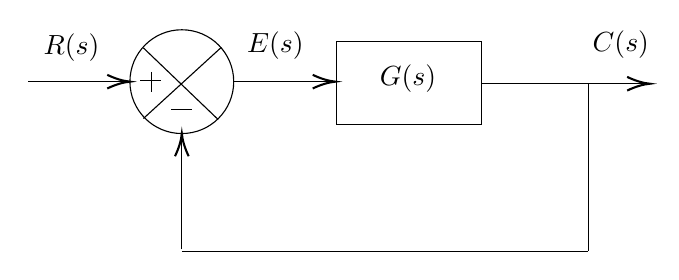
\begin{tikzpicture}[x=0.75pt,y=0.75pt,yscale=-1,xscale=1]
%uncomment if require: \path (0,515); %set diagram left start at 0, and has height of 515
%Shape: Circle [id:dp4181485712735933] 
\draw   (100,149) .. controls (100,135.19) and (111.19,124) .. (125,124) .. controls (138.81,124) and (150,135.19) .. (150,149) .. controls (150,162.81) and (138.81,174) .. (125,174) .. controls (111.19,174) and (100,162.81) .. (100,149) -- cycle ;
%Straight Lines [id:da4740649733052047] 
\draw    (51,149) -- (98,149) ;
\draw [shift={(100,149)}, rotate = 180] [color={rgb, 255:red, 0; green, 0; blue, 0 }  ][line width=0.75]    (10.93,-3.29) .. controls (6.95,-1.4) and (3.31,-0.3) .. (0,0) .. controls (3.31,0.3) and (6.95,1.4) .. (10.93,3.29)   ;
%Straight Lines [id:da3499230348244544] 
\draw    (150,149) -- (197,149) ;
\draw [shift={(199,149)}, rotate = 180] [color={rgb, 255:red, 0; green, 0; blue, 0 }  ][line width=0.75]    (10.93,-3.29) .. controls (6.95,-1.4) and (3.31,-0.3) .. (0,0) .. controls (3.31,0.3) and (6.95,1.4) .. (10.93,3.29)   ;
%Shape: Rectangle [id:dp720053978182877] 
\draw   (199.5,129.5) -- (269.5,129.5) -- (269.5,169.5) -- (199.5,169.5) -- cycle ;
%Straight Lines [id:da444930263203553] 
\draw    (269.5,150) -- (348.5,150) ;
\draw [shift={(350.5,150)}, rotate = 180] [color={rgb, 255:red, 0; green, 0; blue, 0 }  ][line width=0.75]    (10.93,-3.29) .. controls (6.95,-1.4) and (3.31,-0.3) .. (0,0) .. controls (3.31,0.3) and (6.95,1.4) .. (10.93,3.29)   ;
%Straight Lines [id:da11472626901203187] 
\draw    (321,150.25) -- (321,230.75) ;
%Straight Lines [id:da4509078916088618] 
\draw    (125,230.75) -- (320.5,230.75) ;
%Straight Lines [id:da2451181139005163] 
\draw    (125,229.75) -- (125,176) ;
\draw [shift={(125,174)}, rotate = 450] [color={rgb, 255:red, 0; green, 0; blue, 0 }  ][line width=0.75]    (10.93,-3.29) .. controls (6.95,-1.4) and (3.31,-0.3) .. (0,0) .. controls (3.31,0.3) and (6.95,1.4) .. (10.93,3.29)   ;
%Straight Lines [id:da9337473628239266] 
\draw    (106.5,132.75) -- (142.5,167.25) ;
%Straight Lines [id:da5043252444487525] 
\draw    (144,132.5) -- (106.5,166.75) ;
%Straight Lines [id:da8451547864563302] 
\draw    (105,148.5) -- (115,148.5) ;
%Straight Lines [id:da7484338496828458] 
\draw    (110.5,144.25) -- (110.5,153.75) ;
%Straight Lines [id:da9743377983002497] 
\draw    (120,162.5) -- (130,162.5) ;
% Text Node
\draw (57.14,124.69) node [anchor=north west][inner sep=0.75pt]    {$R( s)$};
% Text Node
\draw (219.14,139.54) node [anchor=north west][inner sep=0.75pt]    {$G( s)$};
% Text Node
\draw (321.71,123.26) node [anchor=north west][inner sep=0.75pt]    {$C( s)$};
% Text Node
\draw (155.14,123.54) node [anchor=north west][inner sep=0.75pt]    {$E( s)$};
\end{tikzpicture}
\end{center}

\begin{itemize}
    \item R(s) is a unit parabolic input, $\therefore R(s) = \displaystyle\frac{1}{s^3}$
    \item Closed Loop Transfer Function:
    $$\frac{C(s)}{R(s)} = \frac{G(s)}{1+G(s)}$$
    \item Error function, $E(s)$:
    \begin{align*}
        \frac{E(s)}{R(s)} &= 1-\frac{C(s)}{R(s)} = \frac{1}{1+G(s)}\\
        E(s) &= R(s)\frac{E(s)}{R(s)} = \frac{1}{s^3(1+G(s))}
    \end{align*}
    \item Steady state error, $e_{ss}$:
     \begin{align*}
        e_{ss} &= \lim_{s\to 0}sE(s)\\
        &= \lim_{s\to 0}\frac{1}{s^2(1+G(s))}\\
        &= \frac{1}{K_A}
    \end{align*}
    \item Static Acceleration Error Constant, $K_A$:
    $$K_A = \lim_{s\to 0}s^2G(s)$$
\end{itemize}

\subsection{System Types and Steady State Errors}
\begin{table}[H]
\centering\makegapedcells
\begin{tabular}{c|c|c|c|}
\cline{2-4}
                                    & \multicolumn{3}{c|}{Steady state error, $e_{ss}$}                                                                                                                                                           \\ \cline{2-4} 
                                    & \begin{tabular}[c]{@{}c@{}}Step input\\ $r(t) = 1$\end{tabular} & \begin{tabular}[c]{@{}c@{}}Ramp input\\ $r(t)=t$\end{tabular} & \begin{tabular}[c]{@{}c@{}}Parabolic input\\ $r(t) = 0.5t^2$\end{tabular} \\ \hline
\multicolumn{1}{|c|}{Type 0 System} & $\displaystyle\frac{1}{1+K_P}$                                  & -                                                             & -                                                                         \\ \hline
\multicolumn{1}{|c|}{Type 1 System} & -                                                               & $\displaystyle\frac{1}{K_V}$                                  & -                                                                         \\ \hline
\multicolumn{1}{|c|}{Type 2 System} & -                                                               & -                                                             & $\displaystyle\frac{1}{K_A}$                                                \\ \hline
\end{tabular}
\end{table}
\begin{itemize}
    \item To reduce steady state error $e_{ss}$, increase error constants $K_P$, $K_V$ or $K_A$.
    \item Another way is to add integrators $\displaystyle\frac{1}{s}$ in feed forward path.
    \begin{itemize}[label=$\circ$]
        \item However it reduces system stability.
    \end{itemize}
\end{itemize}

\newpage
\section{W11: Root Locus}
\subsection{Root Locus Method}
\begin{center}
\tikzset{every picture/.style={line width=0.75pt}} %set default line width to 0.75pt        

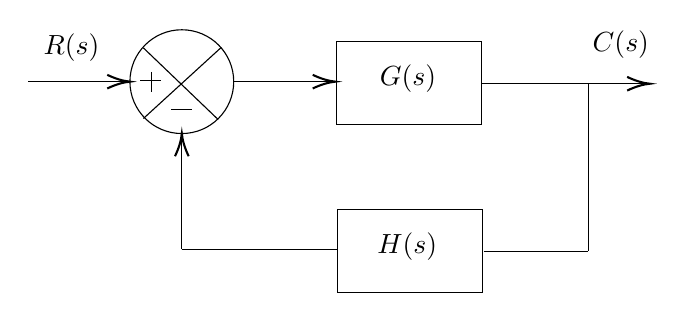
\begin{tikzpicture}[x=0.75pt,y=0.75pt,yscale=-1,xscale=1]
%uncomment if require: \path (0,515); %set diagram left start at 0, and has height of 515

%Shape: Circle [id:dp4181485712735933] 
\draw   (100,149) .. controls (100,135.19) and (111.19,124) .. (125,124) .. controls (138.81,124) and (150,135.19) .. (150,149) .. controls (150,162.81) and (138.81,174) .. (125,174) .. controls (111.19,174) and (100,162.81) .. (100,149) -- cycle ;
%Straight Lines [id:da4740649733052047] 
\draw    (51,149) -- (98,149) ;
\draw [shift={(100,149)}, rotate = 180] [color={rgb, 255:red, 0; green, 0; blue, 0 }  ][line width=0.75]    (10.93,-3.29) .. controls (6.95,-1.4) and (3.31,-0.3) .. (0,0) .. controls (3.31,0.3) and (6.95,1.4) .. (10.93,3.29)   ;
%Straight Lines [id:da3499230348244544] 
\draw    (150,149) -- (197,149) ;
\draw [shift={(199,149)}, rotate = 180] [color={rgb, 255:red, 0; green, 0; blue, 0 }  ][line width=0.75]    (10.93,-3.29) .. controls (6.95,-1.4) and (3.31,-0.3) .. (0,0) .. controls (3.31,0.3) and (6.95,1.4) .. (10.93,3.29)   ;
%Shape: Rectangle [id:dp720053978182877] 
\draw   (199.5,129.5) -- (269.5,129.5) -- (269.5,169.5) -- (199.5,169.5) -- cycle ;
%Straight Lines [id:da444930263203553] 
\draw    (269.5,150) -- (348.5,150) ;
\draw [shift={(350.5,150)}, rotate = 180] [color={rgb, 255:red, 0; green, 0; blue, 0 }  ][line width=0.75]    (10.93,-3.29) .. controls (6.95,-1.4) and (3.31,-0.3) .. (0,0) .. controls (3.31,0.3) and (6.95,1.4) .. (10.93,3.29)   ;
%Straight Lines [id:da11472626901203187] 
\draw    (321,150.25) -- (321,230.75) ;
%Straight Lines [id:da39388134421732124] 
\draw    (270.5,230.75) -- (320.5,230.75) ;
%Shape: Rectangle [id:dp21026770917278692] 
\draw   (200,210.5) -- (270,210.5) -- (270,250.5) -- (200,250.5) -- cycle ;
%Straight Lines [id:da4509078916088618] 
\draw    (125,229.75) -- (200,229.75) ;
%Straight Lines [id:da2451181139005163] 
\draw    (125,229.75) -- (125,176) ;
\draw [shift={(125,174)}, rotate = 450] [color={rgb, 255:red, 0; green, 0; blue, 0 }  ][line width=0.75]    (10.93,-3.29) .. controls (6.95,-1.4) and (3.31,-0.3) .. (0,0) .. controls (3.31,0.3) and (6.95,1.4) .. (10.93,3.29)   ;
%Straight Lines [id:da9337473628239266] 
\draw    (106.5,132.75) -- (142.5,167.25) ;
%Straight Lines [id:da5043252444487525] 
\draw    (144,132.5) -- (106.5,166.75) ;
%Straight Lines [id:da8451547864563302] 
\draw    (105,148.5) -- (115,148.5) ;
%Straight Lines [id:da7484338496828458] 
\draw    (110.5,144.25) -- (110.5,153.75) ;
%Straight Lines [id:da9743377983002497] 
\draw    (120,162.5) -- (130,162.5) ;

% Text Node
\draw (57.14,124.69) node [anchor=north west][inner sep=0.75pt]{$R(s)$};
% Text Node
\draw (219.14,139.54) node [anchor=north west][inner sep=0.75pt]{$G(s)$};
% Text Node
\draw (321.71,123.26) node [anchor=north west][inner sep=0.75pt]{$C(s)$};
% Text Node
\draw (218,220.69) node [anchor=north west][inner sep=0.75pt]{$H(s)$};
\end{tikzpicture}
\end{center}

\begin{itemize}
    \item Closed Loop Transfer Function: \quad$\displaystyle\frac{C(s)}{R(s)} = \frac{G(s)}{1+G(s)H(s)}$
    \item Characteristic Equation: \quad$1+G(s)H(s) = 0$\qquad$\Rightarrow G(s)H(s) = -1$
    \begin{itemize}[label=$\circ$]
        \item We rewrite $G(s)H(s)$ in polynomial form with amplitude $K$, zeros and poles.
        \begin{align*}
            K\frac{N(s)}{D(s)} &= -1\\
            \therefore K\frac{(s+z_1)(s+z_2)\cdots(s+z_m)}{(s+p_1)(s+p_2)\cdots(s+p_n)} &= -1
        \end{align*}
    \end{itemize}
    \item Steps to construct Root Locus:
    \begin{enumerate}
        \item Write characteristic equation in Root Locus form.
        \item Locate open loop poles and zeros.
        \item Find the number of loci and root loci on the real axis.
        \item Determine asymptotes of root locus.
        \item Locate break points.
        \item Derive the departure and arrival angles.
        \begin{itemize}[label=$\circ$]
            \item Complex poles and zeros only
        \end{itemize}
        \item Determine where the root loci crosses the imaginary axis.
        \item Locate closed loop poles for a certain value of $K$.
    \end{enumerate}
\end{itemize}

\subsection{Step 1: Characteristic Equation in Root Locus form}
\begin{itemize}
    \item CE not in RL form: e.g. $1+G(s)H(s) = 0$
    \item General RL form: $1+K\displaystyle\frac{N(s)}{D(s)} = 0$
    \item \textbf{CE in RL form:} e.g. $1+K\displaystyle\frac{s}{(s+1)(s+1)} = 0$
\end{itemize}

\subsection{Step 2: Open Loop Poles and Zeros}
\begin{itemize}
    \item e.g. CE: $1+K\displaystyle\frac{1}{s(s+1)(s+2)}$
    \item $N(s) = 1$
    \item $D(s) = s(s+1)(s+2)$
    \item \textbf{Open Loop Zeros:} no zeros
    \item \textbf{Open Loop Poles:} $s = 0,\ s = -1,\ s = -2$
\end{itemize}

\subsection{Step 3: No. of Loci \& Real Axis Loci}
\begin{itemize}
    \item No. of loci = no. of open loop poles
    \item Real axis loci lies to the left of \textcolor{red}{ODD} no. of poles and zeros on real axis
    \item e.g.\vspace{0.5cm}\\ 
    \begin{minipage}{0.35\textwidth}
    \begin{itemize}[label=$\circ$]
        \item Open loop zeros: $s = -2,\ s = -3$
        \item Open loop poles: $s = 0,\ s = -1$
        \item 2 poles $\Rightarrow$ 2 loci
    \end{itemize}
    \end{minipage}
    \begin{minipage}{0.65\textwidth}
        \begin{center}
        \tikzset{every picture/.style={line width=0.75pt}} %set default line width to 0.75pt
        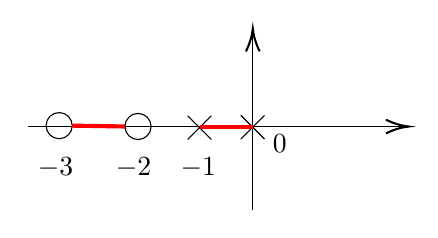
\begin{tikzpicture}[x=0.75pt,y=0.75pt,yscale=-1,xscale=1]
        %uncomment if require: \path (0,300); %set diagram left start at 0, and has height of 300
        %Straight Lines [id:da8408156201083972] 
        \draw    (250,168.4) -- (250,83.2) ;
        \draw [shift={(250,81.2)}, rotate = 450] [color={rgb, 255:red, 0; green, 0; blue, 0 }  ][line width=0.75]    (10.93,-3.29) .. controls (6.95,-1.4) and (3.31,-0.3) .. (0,0) .. controls (3.31,0.3) and (6.95,1.4) .. (10.93,3.29)   ;
        %Straight Lines [id:da645479519102675] 
        \draw    (141.8,128.33) -- (323.08,128.33) ;
        \draw [shift={(325.08,128.33)}, rotate = 180] [color={rgb, 255:red, 0; green, 0; blue, 0 }  ][line width=0.75]    (10.93,-3.29) .. controls (6.95,-1.4) and (3.31,-0.3) .. (0,0) .. controls (3.31,0.3) and (6.95,1.4) .. (10.93,3.29)   ;
        \draw   (244.21,122.92) -- (255.65,134.36)(255.65,122.92) -- (244.21,134.36) ;
        \draw   (218.61,123.12) -- (230.05,134.56)(230.05,123.12) -- (218.61,134.56) ;
        %Shape: Circle [id:dp33815900334124804] 
        \draw   (188.4,128.3) .. controls (188.4,124.82) and (191.22,122) .. (194.7,122) .. controls (198.18,122) and (201,124.82) .. (201,128.3) .. controls (201,131.78) and (198.18,134.6) .. (194.7,134.6) .. controls (191.22,134.6) and (188.4,131.78) .. (188.4,128.3) -- cycle ;
        %Shape: Circle [id:dp5862301162984207] 
        \draw   (150.4,127.9) .. controls (150.4,124.42) and (153.22,121.6) .. (156.7,121.6) .. controls (160.18,121.6) and (163,124.42) .. (163,127.9) .. controls (163,131.38) and (160.18,134.2) .. (156.7,134.2) .. controls (153.22,134.2) and (150.4,131.38) .. (150.4,127.9) -- cycle ;
        %Straight Lines [id:da7836188824968111] 
        \draw [color={rgb, 255:red, 255; green, 0; blue, 0 }  ,draw opacity=1 ][line width=1.5]    (224.6,128.4) -- (250.2,128.4) ;
        %Straight Lines [id:da4869021108607854] 
        \draw [color={rgb, 255:red, 255; green, 0; blue, 0 }  ,draw opacity=1 ][line width=1.5]    (163,127.9) -- (188.4,128.3) ;
        % Text Node
        \draw (214,142) node [anchor=north west][inner sep=0.75pt]    {$-1$};
        % Text Node
        \draw (258.4,131.2) node [anchor=north west][inner sep=0.75pt]    {$0$};
        % Text Node
        \draw (182.8,142) node [anchor=north west][inner sep=0.75pt]    {$-2$};
        % Text Node
        \draw (145.2,142) node [anchor=north west][inner sep=0.75pt]    {$-3$};
        \end{tikzpicture}
        \end{center}
    \end{minipage}
\end{itemize}

\subsection{Step 4: Asymptotes of Root Loci}
\begin{itemize}
    \item Find center of asymptotes on real axis $\sigma_c$ and angle of asymptotes $\beta$.
    \item e.g.\vspace{0.5cm}\\
    \begin{minipage}{0.4\textwidth}
        \begin{itemize}[label=$\circ$]
            \item Open loop zeros: $s = -2$
            \item Open loop poles: $s = 0,\ s = 0,\ s = -4$
            \item No. of open loop zeros, $m = 1$
            \item No. of open loop poles, $n = 3$
        \end{itemize}
    \end{minipage}
    \begin{minipage}{0.6\textwidth}
    \begin{center}
    \tikzset{every picture/.style={line width=0.75pt}} %set default line width to 0.75pt        
    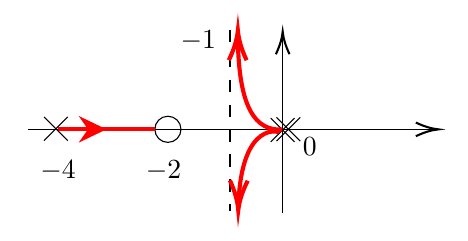
\begin{tikzpicture}[x=0.75pt,y=0.75pt,yscale=-1,xscale=1]
    %uncomment if require: \path (0,300); %set diagram left start at 0, and has height of 300
    %Straight Lines [id:da8408156201083972] 
    \draw    (250,168.4) -- (250,83.2) ;
    \draw [shift={(250,81.2)}, rotate = 450] [color={rgb, 255:red, 0; green, 0; blue, 0 }  ][line width=0.75]    (10.93,-3.29) .. controls (6.95,-1.4) and (3.31,-0.3) .. (0,0) .. controls (3.31,0.3) and (6.95,1.4) .. (10.93,3.29)   ;
    %Straight Lines [id:da645479519102675] 
    \draw    (127.4,128.33) -- (323.08,128.33) ;
    \draw [shift={(325.08,128.33)}, rotate = 180] [color={rgb, 255:red, 0; green, 0; blue, 0 }  ][line width=0.75]    (10.93,-3.29) .. controls (6.95,-1.4) and (3.31,-0.3) .. (0,0) .. controls (3.31,0.3) and (6.95,1.4) .. (10.93,3.29)   ;
    \draw   (244.21,122.92) -- (255.65,134.36)(255.65,122.92) -- (244.21,134.36) ;
    %Shape: Circle [id:dp33815900334124804] 
    \draw   (188.4,128.3) .. controls (188.4,124.82) and (191.22,122) .. (194.7,122) .. controls (198.18,122) and (201,124.82) .. (201,128.3) .. controls (201,131.78) and (198.18,134.6) .. (194.7,134.6) .. controls (191.22,134.6) and (188.4,131.78) .. (188.4,128.3) -- cycle ;
    %Straight Lines [id:da4869021108607854] 
    \draw [color={rgb, 255:red, 255; green, 0; blue, 0 }  ,draw opacity=1 ][line width=1.5]    (141.8,128.3) -- (188.4,128.3) ;
    \draw [shift={(165.1,128.3)}, rotate = 180] [fill={rgb, 255:red, 255; green, 0; blue, 0 }  ,fill opacity=1 ][line width=0.08]  [draw opacity=0] (13.4,-6.43) -- (0,0) -- (13.4,6.44) -- (8.9,0) -- cycle    ;
    %Straight Lines [id:da7769352785714405] 
    \draw  [dash pattern={on 4.5pt off 4.5pt}]  (224.6,80.4) -- (224.6,167.6) ;
    \draw   (247.01,122.52) -- (258.45,133.96)(258.45,122.52) -- (247.01,133.96) ;
    \draw   (135.01,122.32) -- (146.45,133.76)(146.45,122.32) -- (135.01,133.76) ;
    %Curve Lines [id:da5708383735476714] 
    \draw [color={rgb, 255:red, 255; green, 0; blue, 0 }  ,draw opacity=1 ][line width=1.5]    (249.8,128.4) .. controls (236.93,129.18) and (228.62,118.17) .. (228.4,83.51) ;
    \draw [shift={(228.4,80.8)}, rotate = 450.31] [color={rgb, 255:red, 255; green, 0; blue, 0 }  ,draw opacity=1 ][line width=1.5]    (14.21,-4.28) .. controls (9.04,-1.82) and (4.3,-0.39) .. (0,0) .. controls (4.3,0.39) and (9.04,1.82) .. (14.21,4.28)   ;
    %Curve Lines [id:da23714039429295508] 
    \draw [color={rgb, 255:red, 255; green, 0; blue, 0 }  ,draw opacity=1 ][line width=1.5]    (248.2,130) .. controls (249.77,129.61) and (230.21,122.69) .. (228.67,164.57) ;
    \draw [shift={(228.6,167.2)}, rotate = 271.02] [color={rgb, 255:red, 255; green, 0; blue, 0 }  ,draw opacity=1 ][line width=1.5]    (14.21,-4.28) .. controls (9.04,-1.82) and (4.3,-0.39) .. (0,0) .. controls (4.3,0.39) and (9.04,1.82) .. (14.21,4.28)   ;
    % Text Node
    \draw (199.6,79.6) node [anchor=north west][inner sep=0.75pt]    {$-1$};
    % Text Node
    \draw (258.4,131.2) node [anchor=north west][inner sep=0.75pt]    {$0$};
    % Text Node
    \draw (182.8,142.2) node [anchor=north west][inner sep=0.75pt]    {$-2$};
    % Text Node
    \draw (132,142.2) node [anchor=north west][inner sep=0.75pt]    {$-4$};
    \end{tikzpicture}
    \end{center}
    \end{minipage}
    \begin{align*}
        \sigma_c &= \frac{\sum_{i=1}^n p_i-\sum_{i=1}^m z_i}{n-m} = \frac{(0+0-4)-(-2)}{3-1} = -1\\[1em]
        \beta &= \frac{(2\ell+1)180^\circ}{n-m} = \frac{(2\ell+1)180^\circ}{3-1} = 90^\circ,\ -90^\circ
    \end{align*}
\end{itemize}

\subsection{Step 5: Locate Break Points}
\begin{itemize}
    \item Breakaway point: root locus on real axis $\rightarrow$ complex plane
    \item Breakin point: root locus on complex plane $\rightarrow$ real axis
    \item Find corresponding value of $s$ at breakaway/breakin point:
    \item e.g. $N(s) = 1,\ D(s) = s^3+3s^2+2s$\vspace{-0.6cm}\\
    \begin{minipage}{0.3\textwidth}
        \begin{align*}
            \Rightarrow \frac{dK}{ds} = -\frac{D'(s)N(s)-D(s)N'(s)}{N^2(s)} &= 0\\
            D'(s)N(s)-D(s)N'(s) =(3s^2+6s+2)(1) &= 0\\
            \therefore s = -0.4226,\ s &= -1.5774
        \end{align*}
    \end{minipage}
    \begin{minipage}{0.7\textwidth}
    \begin{center}
        \tikzset{every picture/.style={line width=0.75pt}} %set default line width to 0.75pt        
        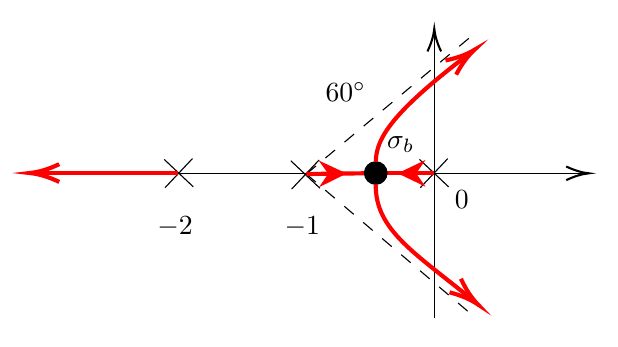
\begin{tikzpicture}[x=0.75pt,y=0.75pt,yscale=-1,xscale=1]
        %uncomment if require: \path (0,300); %set diagram left start at 0, and has height of 300
        %Straight Lines [id:da2806876013403574] 
        \draw    (331.33,180.67) -- (331.33,43.33) ;
        \draw [shift={(331.33,41.33)}, rotate = 450] [color={rgb, 255:red, 0; green, 0; blue, 0 }  ][line width=0.75]    (10.93,-3.29) .. controls (6.95,-1.4) and (3.31,-0.3) .. (0,0) .. controls (3.31,0.3) and (6.95,1.4) .. (10.93,3.29)   ;
        %Straight Lines [id:da3714136380417976] 
        \draw    (186.33,111) -- (403.83,111) ;
        \draw [shift={(405.83,111)}, rotate = 180] [color={rgb, 255:red, 0; green, 0; blue, 0 }  ][line width=0.75]    (10.93,-3.29) .. controls (6.95,-1.4) and (3.31,-0.3) .. (0,0) .. controls (3.31,0.3) and (6.95,1.4) .. (10.93,3.29)   ;
        \draw   (324.61,117.92) -- (337.84,103.89)(324.21,104.3) -- (338.24,117.52) ;
        \draw   (262.61,118.59) -- (275.84,104.56)(262.21,104.96) -- (276.24,118.19) ;
        \draw   (201.61,117.92) -- (214.84,103.89)(201.21,104.3) -- (215.24,117.52) ;
        %Straight Lines [id:da3077611404080487] 
        \draw  [dash pattern={on 4.5pt off 4.5pt}]  (269.67,111.33) -- (350.33,44) ;
        %Straight Lines [id:da14484343536290867] 
        \draw  [dash pattern={on 4.5pt off 4.5pt}]  (269.67,111.33) -- (349.67,179.33) ;
        %Straight Lines [id:da745071564646395] 
        \draw [color={rgb, 255:red, 255; green, 0; blue, 0 }  ,draw opacity=1 ][line width=1.5]    (207.86,110.86) -- (139.43,110.86) ;
        \draw [shift={(136.43,110.86)}, rotate = 360] [color={rgb, 255:red, 255; green, 0; blue, 0 }  ,draw opacity=1 ][line width=1.5]    (14.21,-4.28) .. controls (9.04,-1.82) and (4.3,-0.39) .. (0,0) .. controls (4.3,0.39) and (9.04,1.82) .. (14.21,4.28)   ;
        %Straight Lines [id:da9570790407071053] 
        \draw [color={rgb, 255:red, 255; green, 0; blue, 0 }  ,draw opacity=1 ][line width=1.5]    (269.67,111.33) -- (308.57,110.86) ;
        \draw [shift={(289.12,111.1)}, rotate = 539.3] [fill={rgb, 255:red, 255; green, 0; blue, 0 }  ,fill opacity=1 ][line width=0.08]  [draw opacity=0] (13.4,-6.43) -- (0,0) -- (13.4,6.44) -- (8.9,0) -- cycle    ;
        %Straight Lines [id:da5542680561953961] 
        \draw [color={rgb, 255:red, 255; green, 0; blue, 0 }  ,draw opacity=1 ][line width=1.5]    (296.08,111) -- (331.33,111) ;
        \draw [shift={(313.71,111)}, rotate = 0] [fill={rgb, 255:red, 255; green, 0; blue, 0 }  ,fill opacity=1 ][line width=0.08]  [draw opacity=0] (13.4,-6.43) -- (0,0) -- (13.4,6.44) -- (8.9,0) -- cycle    ;
        %Shape: Circle [id:dp6628621474900558] 
        \draw  [fill={rgb, 255:red, 0; green, 0; blue, 0 }  ,fill opacity=1 ] (297.71,110.86) .. controls (297.71,107.86) and (300.14,105.43) .. (303.14,105.43) .. controls (306.14,105.43) and (308.57,107.86) .. (308.57,110.86) .. controls (308.57,113.86) and (306.14,116.29) .. (303.14,116.29) .. controls (300.14,116.29) and (297.71,113.86) .. (297.71,110.86) -- cycle ;
        %Curve Lines [id:da41659103894647354] 
        \draw [color={rgb, 255:red, 255; green, 0; blue, 0 }  ,draw opacity=1 ][line width=1.5]    (303.14,105.43) .. controls (303.33,94.39) and (310.38,82.01) .. (348.31,53.28) ;
        \draw [shift={(350.67,51.5)}, rotate = 503.13] [color={rgb, 255:red, 255; green, 0; blue, 0 }  ,draw opacity=1 ][line width=1.5]    (14.21,-4.28) .. controls (9.04,-1.82) and (4.3,-0.39) .. (0,0) .. controls (4.3,0.39) and (9.04,1.82) .. (14.21,4.28)   ;
        %Curve Lines [id:da522193690250556] 
        \draw [color={rgb, 255:red, 255; green, 0; blue, 0 }  ,draw opacity=1 ][line width=1.5]    (303.14,116.29) .. controls (302.68,138.59) and (322.95,149.93) .. (350.22,172.41) ;
        \draw [shift={(352.33,174.17)}, rotate = 219.87] [color={rgb, 255:red, 255; green, 0; blue, 0 }  ,draw opacity=1 ][line width=1.5]    (14.21,-4.28) .. controls (9.04,-1.82) and (4.3,-0.39) .. (0,0) .. controls (4.3,0.39) and (9.04,1.82) .. (14.21,4.28)   ;
        % Text Node
        \draw (340,118.07) node [anchor=north west][inner sep=0.75pt]    {$0$};
        % Text Node
        \draw (277.67,66.07) node [anchor=north west][inner sep=0.75pt]    {$60^{\circ }$};
        % Text Node
        \draw (307.38,92) node [anchor=north west][inner sep=0.75pt]    {$\sigma _{b}$};
        % Text Node
        \draw (258,130.75) node [anchor=north west][inner sep=0.75pt]    {$-1$};
        % Text Node
        \draw (196.67,130.75) node [anchor=north west][inner sep=0.75pt]    {$-2$};
        \end{tikzpicture}
    \end{center}
    \end{minipage}
    \item Check break points (K must be positive)
    \begin{align*}
        s &= -0.4226 \quad\Rightarrow K = -\frac{D(s)}{N(s)} = 0.3849\\
        s &= -1.5774 \quad\Rightarrow K = -\frac{D(s)}{N(s)} = -0.3849\ (\text{rej.} \because K > 0)\\
        \therefore \text{Breakaway point, } \sigma_b &= -0.4226
    \end{align*}
\end{itemize}

\subsection{Step 6: Departure \& Arrival Angles}
\begin{itemize}
    \item Root locus `departs' from complex poles
    \item Root locus `arrives' from complex zeros
    \item Departure angle, $\theta_D = 180^\circ +\angle \left[\displaystyle\frac{N(s)}{D(s)}\right]^{'}$
    \item Arrival angle, $\theta_A = 180^\circ -\angle \left[\displaystyle\frac{N(s)}{D(s)}\right]^{'}$
    \item $\angle \left[\displaystyle\frac{N(s)}{D(s)}\right]^{'}$: phase engle of $\displaystyle\frac{N(s)}{D(s)}$ at complex zero/pole, ignoring contribution of that pole
    \item e.g. CE $=1+K\displaystyle\frac{(s+2)}{(s+1+j)(s+1-j)} = 0$\vspace{0.2cm}\\
    OL poles: $s = -1-j,\ s = -1+j$\vspace{-0.2cm}\\
    \begin{minipage}{0.5\textwidth}
    \begin{align*}
        \text{For }s = -1+j,\ \theta_D &= 180^\circ +\angle\left[\frac{N(s)}{D(s)}\right]^{'}\\
        &= 180^\circ + \angle\left.\frac{s+2}{s+1+j}\right|_{s=-1+j}\\
        &= 180^\circ + \angle(-1+j+2)-\angle(-1+j+1+j)\\
        &= 180^\circ + 45^\circ-90^\circ\\
        &= 135^\circ\\
        \text{Similarly for }s = -1-j,\ \theta_D &= -135^\circ.
    \end{align*}
    \end{minipage}
    \begin{minipage}{0.5\textwidth}
    \begin{center}
        \tikzset{every picture/.style={line width=0.75pt}} %set default line width to 0.75pt        

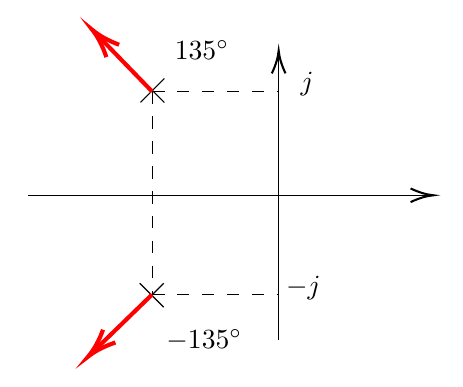
\begin{tikzpicture}[x=0.75pt,y=0.75pt,yscale=-1,xscale=1]
%uncomment if require: \path (0,300); %set diagram left start at 0, and has height of 300

%Straight Lines [id:da2806876013403574] 
\draw    (331.33,180.67) -- (331.33,43.33) ;
\draw [shift={(331.33,41.33)}, rotate = 450] [color={rgb, 255:red, 0; green, 0; blue, 0 }  ][line width=0.75]    (10.93,-3.29) .. controls (6.95,-1.4) and (3.31,-0.3) .. (0,0) .. controls (3.31,0.3) and (6.95,1.4) .. (10.93,3.29)   ;
%Straight Lines [id:da3714136380417976] 
\draw    (210.67,111) -- (403.83,111) ;
\draw [shift={(405.83,111)}, rotate = 180] [color={rgb, 255:red, 0; green, 0; blue, 0 }  ][line width=0.75]    (10.93,-3.29) .. controls (6.95,-1.4) and (3.31,-0.3) .. (0,0) .. controls (3.31,0.3) and (6.95,1.4) .. (10.93,3.29)   ;
%Straight Lines [id:da984347290592247] 
\draw  [dash pattern={on 4.5pt off 4.5pt}]  (270.33,61) -- (270.33,158.83) ;
%Straight Lines [id:da504705901835129] 
\draw  [dash pattern={on 4.5pt off 4.5pt}]  (270.33,61) -- (330.67,61) ;
%Straight Lines [id:da0756953021072555] 
\draw  [dash pattern={on 4.5pt off 4.5pt}]  (270.33,158.83) -- (331.33,158.83) ;
\draw   (264.39,153.39) -- (275.94,164.94)(275.94,153.39) -- (264.39,164.94) ;
\draw   (264.73,54.73) -- (276.27,66.27)(276.27,54.73) -- (264.73,66.27) ;
%Straight Lines [id:da576324161412541] 
\draw [color={rgb, 255:red, 255; green, 0; blue, 0 }  ,draw opacity=1 ][line width=1.5]    (270.33,61) -- (243.59,33.4) ;
\draw [shift={(241.5,31.25)}, rotate = 405.9] [color={rgb, 255:red, 255; green, 0; blue, 0 }  ,draw opacity=1 ][line width=1.5]    (14.21,-4.28) .. controls (9.04,-1.82) and (4.3,-0.39) .. (0,0) .. controls (4.3,0.39) and (9.04,1.82) .. (14.21,4.28)   ;
%Straight Lines [id:da6565054509614499] 
\draw [color={rgb, 255:red, 255; green, 0; blue, 0 }  ,draw opacity=1 ][line width=1.5]    (270.33,158.83) -- (241.65,186.66) ;
\draw [shift={(239.5,188.75)}, rotate = 315.86] [color={rgb, 255:red, 255; green, 0; blue, 0 }  ,draw opacity=1 ][line width=1.5]    (14.21,-4.28) .. controls (9.04,-1.82) and (4.3,-0.39) .. (0,0) .. controls (4.3,0.39) and (9.04,1.82) .. (14.21,4.28)   ;

% Text Node
\draw (340.67,50.4) node [anchor=north west][inner sep=0.75pt]    {$j$};
% Text Node
\draw (333.67,148.73) node [anchor=north west][inner sep=0.75pt]    {$-j$};
% Text Node
\draw (280,35) node [anchor=north west][inner sep=0.75pt]    {$135^{\circ }$};
% Text Node
\draw (276,174.4) node [anchor=north west][inner sep=0.75pt]    {$-135^{\circ }$};
\end{tikzpicture}
    \end{center}
    \end{minipage}
\end{itemize}

\subsection{Step 7: Root Locus Crossing Imaginary Axis}
\begin{itemize}
    \item Find out where root locus crosses the imaginary axis
    \item Substitute $s = j\omega$ into CE
    \item e.g. CE $=1+K\displaystyle\frac{1}{s(s+1)(s+2)} = 0$\\
    \begin{minipage}{0.4\textwidth}
    \begin{align*}
        s(s+1)(s+2)+K &= 0\\
        s^3+3s^2+s+K &= 0\\
        \text{Let }s = j\omega: \quad (j\omega)^3+3(j\omega)^2+2j\omega+K &= 0\\
        (K-3\omega^2)+j(2\omega-\omega^3) &= 0\\
        K-3\omega^2 = 0\quad \text{and}\quad 2\omega-\omega^3 &= 0\\
        \therefore K = 0\text{ when }\omega = 0,\ \text{and } K =6\text{ when } \omega &= \pm\sqrt{2}
    \end{align*}
    \end{minipage}
    \begin{minipage}{0.6\textwidth}
    \begin{center}
        \tikzset{every picture/.style={line width=0.75pt}} %set default line width to 0.75pt        
        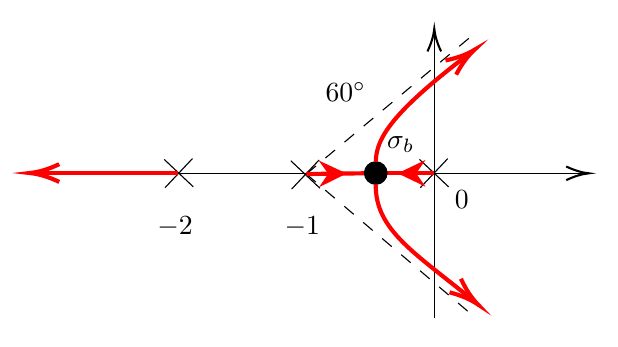
\begin{tikzpicture}[x=0.75pt,y=0.75pt,yscale=-1,xscale=1]
        %uncomment if require: \path (0,300); %set diagram left start at 0, and has height of 300
        %Straight Lines [id:da2806876013403574] 
        \draw    (331.33,180.67) -- (331.33,43.33) ;
        \draw [shift={(331.33,41.33)}, rotate = 450] [color={rgb, 255:red, 0; green, 0; blue, 0 }  ][line width=0.75]    (10.93,-3.29) .. controls (6.95,-1.4) and (3.31,-0.3) .. (0,0) .. controls (3.31,0.3) and (6.95,1.4) .. (10.93,3.29)   ;
        %Straight Lines [id:da3714136380417976] 
        \draw    (186.33,111) -- (403.83,111) ;
        \draw [shift={(405.83,111)}, rotate = 180] [color={rgb, 255:red, 0; green, 0; blue, 0 }  ][line width=0.75]    (10.93,-3.29) .. controls (6.95,-1.4) and (3.31,-0.3) .. (0,0) .. controls (3.31,0.3) and (6.95,1.4) .. (10.93,3.29)   ;
        \draw   (324.61,117.92) -- (337.84,103.89)(324.21,104.3) -- (338.24,117.52) ;
        \draw   (262.61,118.59) -- (275.84,104.56)(262.21,104.96) -- (276.24,118.19) ;
        \draw   (201.61,117.92) -- (214.84,103.89)(201.21,104.3) -- (215.24,117.52) ;
        %Straight Lines [id:da3077611404080487] 
        \draw  [dash pattern={on 4.5pt off 4.5pt}]  (269.67,111.33) -- (350.33,44) ;
        %Straight Lines [id:da14484343536290867] 
        \draw  [dash pattern={on 4.5pt off 4.5pt}]  (269.67,111.33) -- (349.67,179.33) ;
        %Straight Lines [id:da745071564646395] 
        \draw [color={rgb, 255:red, 255; green, 0; blue, 0 }  ,draw opacity=1 ][line width=1.5]    (207.86,110.86) -- (139.43,110.86) ;
        \draw [shift={(136.43,110.86)}, rotate = 360] [color={rgb, 255:red, 255; green, 0; blue, 0 }  ,draw opacity=1 ][line width=1.5]    (14.21,-4.28) .. controls (9.04,-1.82) and (4.3,-0.39) .. (0,0) .. controls (4.3,0.39) and (9.04,1.82) .. (14.21,4.28)   ;
        %Straight Lines [id:da9570790407071053] 
        \draw [color={rgb, 255:red, 255; green, 0; blue, 0 }  ,draw opacity=1 ][line width=1.5]    (269.67,111.33) -- (308.57,110.86) ;
        \draw [shift={(289.12,111.1)}, rotate = 539.3] [fill={rgb, 255:red, 255; green, 0; blue, 0 }  ,fill opacity=1 ][line width=0.08]  [draw opacity=0] (13.4,-6.43) -- (0,0) -- (13.4,6.44) -- (8.9,0) -- cycle    ;
        %Straight Lines [id:da5542680561953961] 
        \draw [color={rgb, 255:red, 255; green, 0; blue, 0 }  ,draw opacity=1 ][line width=1.5]    (296.08,111) -- (331.33,111) ;
        \draw [shift={(313.71,111)}, rotate = 0] [fill={rgb, 255:red, 255; green, 0; blue, 0 }  ,fill opacity=1 ][line width=0.08]  [draw opacity=0] (13.4,-6.43) -- (0,0) -- (13.4,6.44) -- (8.9,0) -- cycle    ;
        %Shape: Circle [id:dp6628621474900558] 
        \draw  [fill={rgb, 255:red, 0; green, 0; blue, 0 }  ,fill opacity=1 ] (297.71,110.86) .. controls (297.71,107.86) and (300.14,105.43) .. (303.14,105.43) .. controls (306.14,105.43) and (308.57,107.86) .. (308.57,110.86) .. controls (308.57,113.86) and (306.14,116.29) .. (303.14,116.29) .. controls (300.14,116.29) and (297.71,113.86) .. (297.71,110.86) -- cycle ;
        %Curve Lines [id:da41659103894647354] 
        \draw [color={rgb, 255:red, 255; green, 0; blue, 0 }  ,draw opacity=1 ][line width=1.5]    (303.14,105.43) .. controls (303.33,94.39) and (310.38,82.01) .. (348.31,53.28) ;
        \draw [shift={(350.67,51.5)}, rotate = 503.13] [color={rgb, 255:red, 255; green, 0; blue, 0 }  ,draw opacity=1 ][line width=1.5]    (14.21,-4.28) .. controls (9.04,-1.82) and (4.3,-0.39) .. (0,0) .. controls (4.3,0.39) and (9.04,1.82) .. (14.21,4.28)   ;
        %Curve Lines [id:da522193690250556] 
        \draw [color={rgb, 255:red, 255; green, 0; blue, 0 }  ,draw opacity=1 ][line width=1.5]    (303.14,116.29) .. controls (302.68,138.59) and (322.95,149.93) .. (350.22,172.41) ;
        \draw [shift={(352.33,174.17)}, rotate = 219.87] [color={rgb, 255:red, 255; green, 0; blue, 0 }  ,draw opacity=1 ][line width=1.5]    (14.21,-4.28) .. controls (9.04,-1.82) and (4.3,-0.39) .. (0,0) .. controls (4.3,0.39) and (9.04,1.82) .. (14.21,4.28)   ;
        % Text Node
        \draw (340,118.07) node [anchor=north west][inner sep=0.75pt]    {$0$};
        % Text Node
        \draw (277.67,66.07) node [anchor=north west][inner sep=0.75pt]    {$60^{\circ }$};
        % Text Node
        \draw (307.38,92) node [anchor=north west][inner sep=0.75pt]    {$\sigma _{b}$};
        % Text Node
        \draw (258,130.75) node [anchor=north west][inner sep=0.75pt]    {$-1$};
        % Text Node
        \draw (196.67,130.75) node [anchor=north west][inner sep=0.75pt]    {$-2$};
        \end{tikzpicture}
    \end{center}
    \end{minipage}
    \item Root locus crosses imaginary axis at $K = 6$ when $\omega = \pm\sqrt{2}$
    \item Root locus touches imaginary axis at $K = 0$ when $\omega = 0$
\end{itemize}
 
\newpage
\subsection{Step 8: Closed Loop Poles and K}
\begin{itemize}
    \item Compute closed loop poles at $s = \Bar{s}$ for a specific $K$
    \item Compute $K$ for a set of closed loop poles at $s = \Bar{s}$
    \item e.g. CE: $\displaystyle 1+K\frac{1}{s(s+1)(s+2)} = 0$\vspace{0.15cm}\\
    We want the closed loop poles to have $\zeta = 0.5$.\\
    At the intersection, $s = -0.3337\pm j0.5780$.\\
    Find value of K and the location of the third pole.
    \begin{align*}
        &K= \left|\frac{D(s)}{N(s)}\right|_{s = -0.337+j0.5780} = 1.0383\\
        &\Rightarrow \quad s^3+3s^2+2s+K = 0\\
        &(s+a_1)(s+0.3337+j0.5780)(s+0.33737-j0.5780) = 0\\
        &\Rightarrow \quad a_1 = 2.3326
    \end{align*}
    \item $\therefore K = 1.0383,$ and the third pole is at $s = 2.3326$.
\end{itemize}

\subsection{Root Locus with P, I and PD Controllers}
\begin{center}
\tikzset{every picture/.style={line width=0.75pt}} %set default line width to 0.75pt        
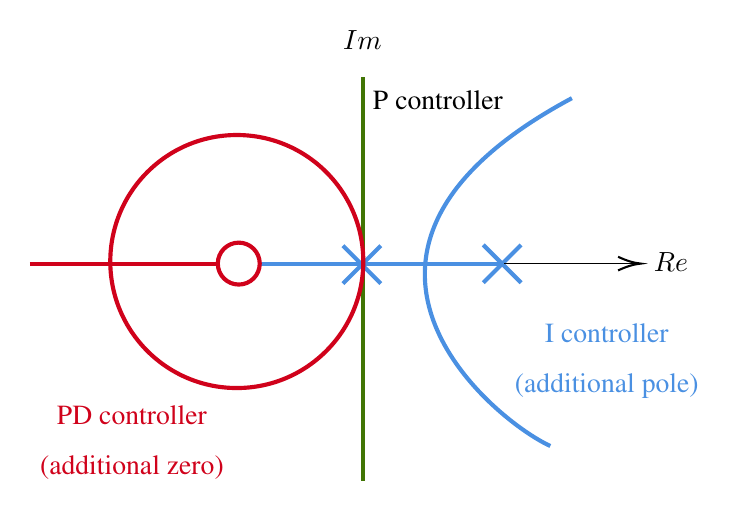
\begin{tikzpicture}[x=0.75pt,y=0.75pt,yscale=-1,xscale=1]
%uncomment if require: \path (0,300); %set diagram left start at 0, and has height of 300
%Straight Lines [id:da573029809593012] 
\draw [color={rgb, 255:red, 65; green, 117; blue, 5 }  ,draw opacity=1 ][line width=1.5]    (290.5,40.75) -- (290.5,235.2) ;
%Straight Lines [id:da6886979309847601] 
\draw [color={rgb, 255:red, 74; green, 144; blue, 226 }  ,draw opacity=1 ][line width=1.5]    (240.6,130.5) -- (358.4,130.5) ;
\draw  [color={rgb, 255:red, 74; green, 144; blue, 226 }  ,draw opacity=1 ][line width=1.5]  (348.3,121.48) -- (366.53,139.72)(366.53,121.48) -- (348.3,139.72) ;
\draw  [color={rgb, 255:red, 74; green, 144; blue, 226 }  ,draw opacity=1 ][line width=1.5]  (280.7,121.88) -- (298.93,140.12)(298.93,121.88) -- (280.7,140.12) ;
%Curve Lines [id:da8930646556729578] 
\draw [color={rgb, 255:red, 74; green, 144; blue, 226 }  ,draw opacity=1 ][line width=1.5]    (391,50.8) .. controls (255,123.6) and (351.4,204.8) .. (380.6,218.4) ;
%Shape: Circle [id:dp9653535007991156] 
\draw  [color={rgb, 255:red, 208; green, 2; blue, 27 }  ,draw opacity=1 ][line width=1.5]  (168.6,129.5) .. controls (168.6,95.84) and (195.89,68.55) .. (229.55,68.55) .. controls (263.21,68.55) and (290.5,95.84) .. (290.5,129.5) .. controls (290.5,163.16) and (263.21,190.45) .. (229.55,190.45) .. controls (195.89,190.45) and (168.6,163.16) .. (168.6,129.5) -- cycle ;
%Shape: Circle [id:dp917640003093716] 
\draw  [color={rgb, 255:red, 208; green, 2; blue, 27 }  ,draw opacity=1 ][line width=1.5]  (220.4,130.5) .. controls (220.4,124.92) and (224.92,120.4) .. (230.5,120.4) .. controls (236.08,120.4) and (240.6,124.92) .. (240.6,130.5) .. controls (240.6,136.08) and (236.08,140.6) .. (230.5,140.6) .. controls (224.92,140.6) and (220.4,136.08) .. (220.4,130.5) -- cycle ;
%Straight Lines [id:da7071043183665768] 
\draw [color={rgb, 255:red, 208; green, 2; blue, 27 }  ,draw opacity=1 ][line width=1.5]    (129.8,130.5) -- (220.4,130.5) ;
%Straight Lines [id:da5011219700266678] 
\draw    (358.4,130.5) -- (422.2,130.5) ;
\draw [shift={(424.2,130.5)}, rotate = 180] [color={rgb, 255:red, 0; green, 0; blue, 0 }  ][line width=0.75]    (10.93,-3.29) .. controls (6.95,-1.4) and (3.31,-0.3) .. (0,0) .. controls (3.31,0.3) and (6.95,1.4) .. (10.93,3.29)   ;
% Text Node
\draw (293.9,45.9) node [anchor=north west][inner sep=0.75pt]   [align=left] {{\fontfamily{ptm}\selectfont P controller}};
% Text Node
\draw (279.5,17.1) node [anchor=north west][inner sep=0.75pt]    {$Im$};
% Text Node
\draw (359.6,158.2) node [anchor=north west][inner sep=0.75pt]  [color={rgb, 255:red, 74; green, 144; blue, 226 }  ,opacity=1 ] [align=left] {\begin{minipage}[lt]{70.42216pt}\setlength\topsep{0pt}
\begin{center}
{\fontfamily{ptm}\selectfont I controller}\\{\fontfamily{ptm}\selectfont (additional pole)}
\end{center}
\end{minipage}};
% Text Node
\draw (429.2,123.8) node [anchor=north west][inner sep=0.75pt]    {$Re$};
% Text Node
\draw (130.8,197.6) node [anchor=north west][inner sep=0.75pt]  [color={rgb, 255:red, 208; green, 2; blue, 27 }  ,opacity=1 ] [align=left] {\begin{minipage}[lt]{70.41196000000001pt}\setlength\topsep{0pt}
\begin{center}
{\fontfamily{ptm}\selectfont PD controller}\\{\fontfamily{ptm}\selectfont (additional zero)}
\end{center}
\end{minipage}};
\end{tikzpicture}
\end{center}

\begin{itemize}
    \item Adding an I controller: introduces a pole at origin
    \item Adding a D controller: introduces a zero
    \begin{itemize}[label=$\circ$]
        \item Location of zero depends on ratio of derivative to proportional gain
    \end{itemize}
\end{itemize}

\newpage
\section{W11: Bode Diagrams}
$$\text{Transfer function, }G(j\omega) = K\frac{N(j\omega)}{D(j\omega)}$$
\begin{itemize}
    \item Transfer function of a LTI system can be represented by a Bode Diagram, made up of 2 diagrams:
    \begin{enumerate}
        \item Magnitude of TF vs Frequency (log-log plot)
        \item Phase angle of TF vs Frequency (log-log plot)
    \end{enumerate}
    \item Magnitude of TF is measured in decibels (dB), where
    \begin{align*}
        20\log_{10}|G(j\omega)| = 20\log_{10}K+20\log_{10}|N(j\omega)|-20\log_{10}|D(j\omega)|.
    \end{align*}
    \item Phase angle is measured in degrees, where $\phi = \angle N(j\omega)-\angle D(j\omega)$.
\end{itemize}

\subsection{Bode Diagram of Constant}
$$G(j\omega) = K,\ K > 0$$
\begin{minipage}{0.35\textwidth}
\begin{itemize}
    \item Magnitude: dB $= 20\log_{10} K$
    \begin{itemize}[label=$\circ$]
        \item If $K > 1,\ 20\log_{10}K > 0$.
        \item If $0<K<1,\ 20\log_{10}K < 0$.
    \end{itemize}
    \item Phase: $\phi = 0$
    \begin{itemize}[label=$\circ$]
        \item Independent of $K,\ \omega$
    \end{itemize}
\end{itemize}
\end{minipage}
\begin{minipage}{0.65\textwidth}
\begin{center}




\tikzset{every picture/.style={line width=0.75pt}} %set default line width to 0.75pt        

\begin{tikzpicture}[x=0.75pt,y=0.75pt,yscale=-1,xscale=1]
%uncomment if require: \path (0,300); %set diagram left start at 0, and has height of 300

%Straight Lines [id:da4926848260262404] 
\draw    (72.5,193.63) -- (72.5,71.66) ;
\draw [shift={(72.5,69.66)}, rotate = 450] [color={rgb, 255:red, 0; green, 0; blue, 0 }  ][line width=0.75]    (10.93,-3.29) .. controls (6.95,-1.4) and (3.31,-0.3) .. (0,0) .. controls (3.31,0.3) and (6.95,1.4) .. (10.93,3.29)   ;
%Straight Lines [id:da41991018488295473] 
\draw    (279.26,192.72) -- (279.26,70.75) ;
\draw [shift={(279.26,68.75)}, rotate = 450] [color={rgb, 255:red, 0; green, 0; blue, 0 }  ][line width=0.75]    (10.93,-3.29) .. controls (6.95,-1.4) and (3.31,-0.3) .. (0,0) .. controls (3.31,0.3) and (6.95,1.4) .. (10.93,3.29)   ;
%Straight Lines [id:da9178045362505265] 
\draw    (72.5,193.63) -- (218.35,193.63) ;
\draw [shift={(220.35,193.63)}, rotate = 180] [color={rgb, 255:red, 0; green, 0; blue, 0 }  ][line width=0.75]    (10.93,-3.29) .. controls (6.95,-1.4) and (3.31,-0.3) .. (0,0) .. controls (3.31,0.3) and (6.95,1.4) .. (10.93,3.29)   ;
%Straight Lines [id:da9264184908369435] 
\draw    (279.26,130.73) -- (425.11,130.73) ;
\draw [shift={(427.11,130.73)}, rotate = 180] [color={rgb, 255:red, 0; green, 0; blue, 0 }  ][line width=0.75]    (10.93,-3.29) .. controls (6.95,-1.4) and (3.31,-0.3) .. (0,0) .. controls (3.31,0.3) and (6.95,1.4) .. (10.93,3.29)   ;
%Straight Lines [id:da8767914274541724] 
\draw [color={rgb, 255:red, 255; green, 0; blue, 0 }  ,draw opacity=1 ][fill={rgb, 255:red, 208; green, 2; blue, 27 }  ,fill opacity=1 ][line width=1.5]    (72.5,131.65) -- (218.79,131.65) ;
%Straight Lines [id:da14957276614916304] 
\draw [color={rgb, 255:red, 255; green, 0; blue, 0 }  ,draw opacity=1 ][fill={rgb, 255:red, 208; green, 2; blue, 27 }  ,fill opacity=1 ][line width=1.5]    (279.26,130.73) -- (425.55,130.73) ;

% Text Node
\draw (5,120.72) node [anchor=north west][inner sep=0.75pt]    {$20\log_{10} K$};
% Text Node
\draw (62.11,50.41) node [anchor=north west][inner sep=0.75pt]   [align=left] {dB};
% Text Node
\draw (222.48,184.43) node [anchor=north west][inner sep=0.75pt]    {$\log \omega $};
% Text Node
\draw (271.59,48.11) node [anchor=north west][inner sep=0.75pt]    {$\phi $};
% Text Node
\draw (434.3,121.76) node [anchor=north west][inner sep=0.75pt]    {$\log \omega $};
% Text Node
\draw (263.89,120.39) node [anchor=north west][inner sep=0.75pt]    {$0$};


\end{tikzpicture}


\end{center}
\end{minipage}

\subsection{Bode Diagram of Integral Factor}
$$G(j\omega) = \frac{1}{j\omega}$$
\begin{minipage}{0.45\textwidth}
\begin{itemize}
    \item Magnitude: dB $=20\log_{10}\left|\displaystyle\frac{1}{j\omega}\right| = -20\log_{10}(\omega)$
    \begin{itemize}[label=$\circ$]
        \item Also known as -20 dB/decade
    \end{itemize}
    \item Phase: $\phi = \angle\displaystyle\frac{1}{j\omega} = -90^\circ$
    \begin{itemize}[label=$\circ$]
        \item Independent of $\omega$
    \end{itemize}
\end{itemize}
\end{minipage}
\begin{minipage}{0.55\textwidth}
\begin{center}
    \tikzset{every picture/.style={line width=0.75pt}} %set default line width to 0.75pt        

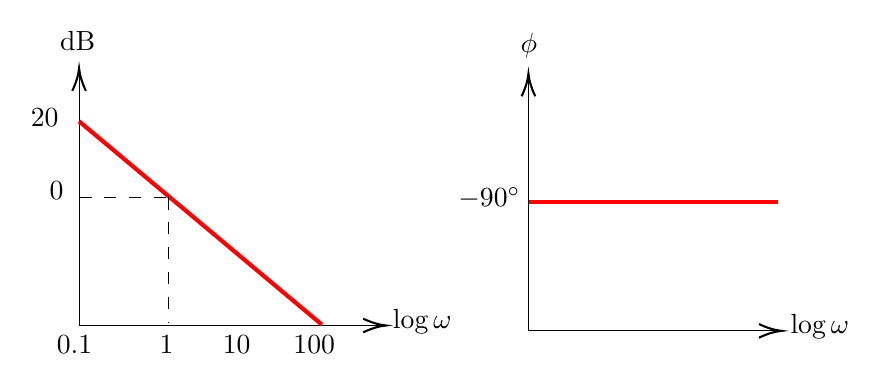
\begin{tikzpicture}[x=0.75pt,y=0.75pt,yscale=-1,xscale=1]
%uncomment if require: \path (0,300); %set diagram left start at 0, and has height of 300

%Straight Lines [id:da14957276614916304] 
\draw [color={rgb, 255:red, 255; green, 0; blue, 0 }  ,draw opacity=1 ][fill={rgb, 255:red, 208; green, 2; blue, 27 }  ,fill opacity=1 ][line width=1.5]    (330,133.23) -- (450,133.23) ;
%Straight Lines [id:da4926848260262404] 
\draw    (113.5,192.63) -- (113.5,70.66) ;
\draw [shift={(113.5,68.66)}, rotate = 450] [color={rgb, 255:red, 0; green, 0; blue, 0 }  ][line width=0.75]    (10.93,-3.29) .. controls (6.95,-1.4) and (3.31,-0.3) .. (0,0) .. controls (3.31,0.3) and (6.95,1.4) .. (10.93,3.29)   ;
%Straight Lines [id:da41991018488295473] 
\draw    (330,195.22) -- (330,73.25) ;
\draw [shift={(330,71.25)}, rotate = 450] [color={rgb, 255:red, 0; green, 0; blue, 0 }  ][line width=0.75]    (10.93,-3.29) .. controls (6.95,-1.4) and (3.31,-0.3) .. (0,0) .. controls (3.31,0.3) and (6.95,1.4) .. (10.93,3.29)   ;
%Straight Lines [id:da9178045362505265] 
\draw    (113.5,192.63) -- (259.35,192.63) ;
\draw [shift={(261.35,192.63)}, rotate = 180] [color={rgb, 255:red, 0; green, 0; blue, 0 }  ][line width=0.75]    (10.93,-3.29) .. controls (6.95,-1.4) and (3.31,-0.3) .. (0,0) .. controls (3.31,0.3) and (6.95,1.4) .. (10.93,3.29)   ;
%Straight Lines [id:da9264184908369435] 
\draw    (330,195.22) -- (450,195.22) ;
\draw [shift={(452,195.22)}, rotate = 180] [color={rgb, 255:red, 0; green, 0; blue, 0 }  ][line width=0.75]    (10.93,-3.29) .. controls (6.95,-1.4) and (3.31,-0.3) .. (0,0) .. controls (3.31,0.3) and (6.95,1.4) .. (10.93,3.29)   ;
%Straight Lines [id:da8767914274541724] 
\draw [color={rgb, 255:red, 255; green, 0; blue, 0 }  ,draw opacity=1 ][fill={rgb, 255:red, 208; green, 2; blue, 27 }  ,fill opacity=1 ][line width=1.5]    (113.5,94.25) -- (230.5,192.25) ;
%Straight Lines [id:da13105716464982198] 
\draw  [dash pattern={on 4.5pt off 4.5pt}]  (156.5,130.75) -- (156.5,191) ;
%Straight Lines [id:da1930065508880232] 
\draw  [dash pattern={on 4.5pt off 4.5pt}]  (113.5,130.75) -- (156.5,130.75) ;

% Text Node
\draw (103.11,49.41) node [anchor=north west][inner sep=0.75pt]   [align=left] {dB};
% Text Node
\draw (263.48,183.43) node [anchor=north west][inner sep=0.75pt]    {$\log \omega $};
% Text Node
\draw (325,50.61) node [anchor=north west][inner sep=0.75pt]    {$\phi $};
% Text Node
\draw (455,185.76) node [anchor=north west][inner sep=0.75pt]    {$\log \omega $};
% Text Node
\draw (295,125) node [anchor=north west][inner sep=0.75pt]    {$-90^{\circ }$};
% Text Node
\draw (89,87) node [anchor=north west][inner sep=0.75pt]    {$20$};
% Text Node
\draw (101.5,196.4) node [anchor=north west][inner sep=0.75pt]    {$0.1$};
% Text Node
\draw (151,196.4) node [anchor=north west][inner sep=0.75pt]    {$1$};
% Text Node
\draw (181.5,196.4) node [anchor=north west][inner sep=0.75pt]    {$10$};
% Text Node
\draw (215.5,196.4) node [anchor=north west][inner sep=0.75pt]    {$100$};
% Text Node
\draw (98,122) node [anchor=north west][inner sep=0.75pt]    {$0$};


\end{tikzpicture}

\end{center}
\end{minipage}

\subsection{Bode Diagram of Derivative Factor}
$$G(j\omega) = j\omega$$
\begin{minipage}{0.35\textwidth}
\begin{itemize}
    \item Magnitude: dB $= 20\log_{10}(j\omega)$\\ $\Rightarrow$ 20 dB/decade
    \item Phase: $\phi = \angle j\omega = 90^\circ$
    \begin{itemize}
        \item Independent of $\omega$
    \end{itemize}
\end{itemize}
\end{minipage}
\begin{minipage}{0.33\textwidth}
\begin{center}
    \tikzset{every picture/.style={line width=0.75pt}} %set default line width to 0.75pt        
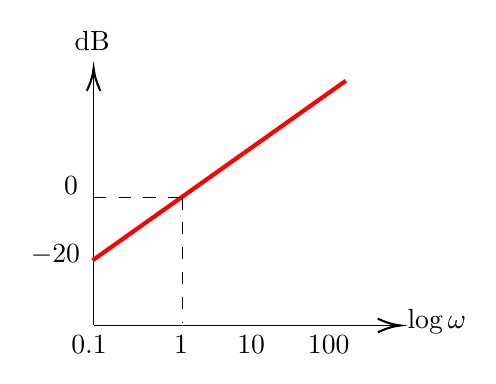
\begin{tikzpicture}[x=0.75pt,y=0.75pt,yscale=-1,xscale=1]
%Straight Lines [id:da20219203487957138] 
\draw    (65.5,209.63) -- (65.5,87.66) ;
\draw [shift={(65.5,85.66)}, rotate = 450] [color={rgb, 255:red, 0; green, 0; blue, 0 }  ][line width=0.75]    (10.93,-3.29) .. controls (6.95,-1.4) and (3.31,-0.3) .. (0,0) .. controls (3.31,0.3) and (6.95,1.4) .. (10.93,3.29)   ;
%Straight Lines [id:da6575334279005483] 
\draw    (65.5,209.63) -- (211.35,209.63) ;
\draw [shift={(213.35,209.63)}, rotate = 180] [color={rgb, 255:red, 0; green, 0; blue, 0 }  ][line width=0.75]    (10.93,-3.29) .. controls (6.95,-1.4) and (3.31,-0.3) .. (0,0) .. controls (3.31,0.3) and (6.95,1.4) .. (10.93,3.29)   ;
%Straight Lines [id:da9197817374376467] 
\draw [color={rgb, 255:red, 255; green, 0; blue, 0 }  ,draw opacity=1 ][fill={rgb, 255:red, 208; green, 2; blue, 27 }  ,fill opacity=1 ][line width=1.5]    (65,178.25) -- (187,91.75) ;
%Straight Lines [id:da6872845798844536] 
\draw  [dash pattern={on 4.5pt off 4.5pt}]  (108.5,147.75) -- (108.5,208) ;
%Straight Lines [id:da5097225638933114] 
\draw  [dash pattern={on 4.5pt off 4.5pt}]  (65.5,147.75) -- (108.5,147.75) ;
% Text Node
\draw (50,136.9) node [anchor=north west][inner sep=0.75pt]    {$0$};
% Text Node
\draw (167.5,213.4) node [anchor=north west][inner sep=0.75pt]    {$100$};
% Text Node
\draw (133.5,213.4) node [anchor=north west][inner sep=0.75pt]    {$10$};
% Text Node
\draw (103,213.4) node [anchor=north west][inner sep=0.75pt]    {$1$};
% Text Node
\draw (53.5,213.4) node [anchor=north west][inner sep=0.75pt]    {$0.1$};
% Text Node
\draw (34,169.4) node [anchor=north west][inner sep=0.75pt]    {$-20$};
% Text Node
\draw (215.48,200.43) node [anchor=north west][inner sep=0.75pt]    {$\log \omega $};
% Text Node
\draw (55.11,66.41) node [anchor=north west][inner sep=0.75pt]   [align=left] {dB};
\end{tikzpicture}
\end{center}
\end{minipage}
\begin{minipage}{0.32\textwidth}
\begin{center}
    
\tikzset{every picture/.style={line width=0.75pt}} %set default line width to 0.75pt        

\begin{tikzpicture}[x=0.75pt,y=0.75pt,yscale=-1,xscale=1]
%uncomment if require: \path (0,300); %set diagram left start at 0, and has height of 300

%Straight Lines [id:da14957276614916304] 
\draw [color={rgb, 255:red, 255; green, 0; blue, 0 }  ,draw opacity=1 ][fill={rgb, 255:red, 208; green, 2; blue, 27 }  ,fill opacity=1 ][line width=1.5]    (371.76,137.23) -- (518.05,137.23) ;
%Straight Lines [id:da41991018488295473] 
\draw    (371.76,199.22) -- (371.76,77.25) ;
\draw [shift={(371.76,75.25)}, rotate = 450] [color={rgb, 255:red, 0; green, 0; blue, 0 }  ][line width=0.75]    (10.93,-3.29) .. controls (6.95,-1.4) and (3.31,-0.3) .. (0,0) .. controls (3.31,0.3) and (6.95,1.4) .. (10.93,3.29)   ;
%Straight Lines [id:da9264184908369435] 
\draw    (371.76,199.22) -- (517.61,199.22) ;
\draw [shift={(519.61,199.22)}, rotate = 180] [color={rgb, 255:red, 0; green, 0; blue, 0 }  ][line width=0.75]    (10.93,-3.29) .. controls (6.95,-1.4) and (3.31,-0.3) .. (0,0) .. controls (3.31,0.3) and (6.95,1.4) .. (10.93,3.29)   ;

% Text Node
\draw (366.09,53.61) node [anchor=north west][inner sep=0.75pt]    {$\phi $};
% Text Node
\draw (527.8,189.76) node [anchor=north west][inner sep=0.75pt]    {$\log \omega $};
% Text Node
\draw (343,128) node [anchor=north west][inner sep=0.75pt]    {$90^{\circ }$};


\end{tikzpicture}
\end{center}
\end{minipage}

\subsection{Bode Diagram of First Order System}
$$G(j\omega) = \frac{1}{Tj\omega+1}$$
\begin{itemize}
    \begin{minipage}{0.55\textwidth}
    \item Magnitude: dB $= 20\log_{10}\left|\displaystyle\frac{1}{Tj\omega+1}\right| = -20\log_{10}\sqrt{T^2\omega^2+1}$
    \begin{itemize}[label=$\circ$]
        \item At low frequency: $\omega \ll \displaystyle\frac{1}{T},\ \text{dB} \approx 0$.
        \item At high frequency: $\omega \gg \displaystyle\frac{1}{T},\ \text{dB}\approx -20\log_{10}T\omega$.\\
        $\Rightarrow$ -20 dB/decade
    \end{itemize}
    \end{minipage}
    \begin{minipage}{0.45\textwidth}
    \begin{center}
        

\tikzset{every picture/.style={line width=0.75pt}} %set default line width to 0.75pt        

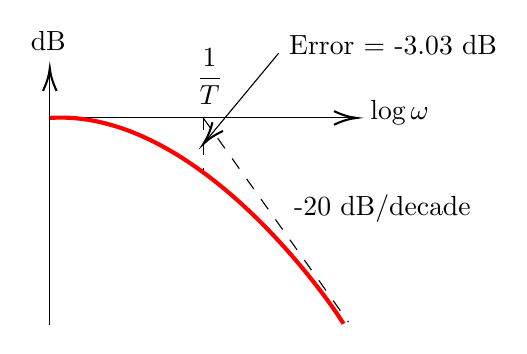
\begin{tikzpicture}[x=0.75pt,y=0.75pt,yscale=-1,xscale=1]
%uncomment if require: \path (0,300); %set diagram left start at 0, and has height of 300

%Straight Lines [id:da20219203487957138] 
\draw    (65.5,209.63) -- (65.5,87.66) ;
\draw [shift={(65.5,85.66)}, rotate = 450] [color={rgb, 255:red, 0; green, 0; blue, 0 }  ][line width=0.75]    (10.93,-3.29) .. controls (6.95,-1.4) and (3.31,-0.3) .. (0,0) .. controls (3.31,0.3) and (6.95,1.4) .. (10.93,3.29)   ;
%Straight Lines [id:da6575334279005483] 
\draw    (65.5,109.63) -- (211.35,109.63) ;
\draw [shift={(213.35,109.63)}, rotate = 180] [color={rgb, 255:red, 0; green, 0; blue, 0 }  ][line width=0.75]    (10.93,-3.29) .. controls (6.95,-1.4) and (3.31,-0.3) .. (0,0) .. controls (3.31,0.3) and (6.95,1.4) .. (10.93,3.29)   ;
%Straight Lines [id:da9896708874073339] 
\draw  [dash pattern={on 4.5pt off 4.5pt}]  (139.43,109.63) -- (209.4,208) ;
%Curve Lines [id:da1524138811680511] 
\draw [color={rgb, 255:red, 255; green, 0; blue, 0 }  ,draw opacity=1 ][line width=1.5]    (65.5,109.63) .. controls (139,104.8) and (205,204.8) .. (207,208.8) ;
%Straight Lines [id:da9088377067311144] 
\draw  [dash pattern={on 4.5pt off 4.5pt}]  (139.43,109.63) -- (139.43,134.8) ;
%Straight Lines [id:da2701365368475739] 
\draw    (175.8,78.4) -- (140.7,120.68) ;
\draw [shift={(139.43,122.22)}, rotate = 309.7] [color={rgb, 255:red, 0; green, 0; blue, 0 }  ][line width=0.75]    (10.93,-3.29) .. controls (6.95,-1.4) and (3.31,-0.3) .. (0,0) .. controls (3.31,0.3) and (6.95,1.4) .. (10.93,3.29)   ;

% Text Node
\draw (218.68,99.63) node [anchor=north west][inner sep=0.75pt]    {$\log \omega $};
% Text Node
\draw (55.11,66.41) node [anchor=north west][inner sep=0.75pt]   [align=left] {dB};
% Text Node
\draw (134.8,75) node [anchor=north west][inner sep=0.75pt]    {$\displaystyle\frac{1}{T}$};
% Text Node
\draw (179.6,68.4) node [anchor=north west][inner sep=0.75pt]   [align=left] {Error = -3.03 dB};
% Text Node
\draw (182,145.6) node [anchor=north west][inner sep=0.75pt]   [align=left] {\mbox{-}20 dB/decade};
\end{tikzpicture}

    \end{center}
    \end{minipage}
    
    \begin{minipage}{0.55\textwidth}
    \item Phase: $\phi =\angle\displaystyle\frac{1}{Tj\omega+1}= -\tan^{-1}\omega T$
    \begin{itemize}[label=$\circ$]
        \item At low frequency: $\phi \approx -\tan^{-1} 0 = 0^\circ$.
        \item At high frequency: $\phi \approx -\tan^{-1} \infty = -90^\circ$.
        \item Asymptotes meet at corner frequency where $\omega = \displaystyle\frac{1}{T}$:\\
        $\phi = -\tan^{-1} 1 = -45^\circ$
    \end{itemize}
    \end{minipage}
    \begin{minipage}{0.45\textwidth}
    \begin{center}
        \tikzset{every picture/.style={line width=0.75pt}} %set default line width to 0.75pt        
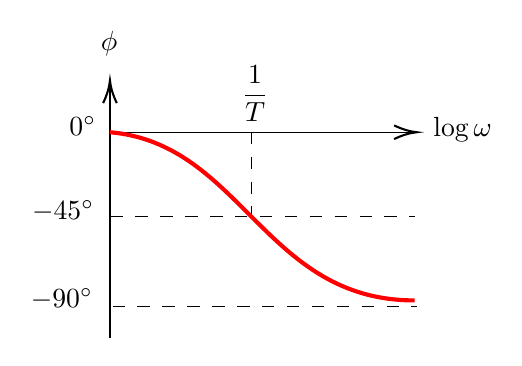
\begin{tikzpicture}[x=0.75pt,y=0.75pt,yscale=-1,xscale=1]
%Straight Lines [id:da41991018488295473] 
\draw    (371.76,199.22) -- (371.76,77.25) ;
\draw [shift={(371.76,75.25)}, rotate = 450] [color={rgb, 255:red, 0; green, 0; blue, 0 }  ][line width=0.75]    (10.93,-3.29) .. controls (6.95,-1.4) and (3.31,-0.3) .. (0,0) .. controls (3.31,0.3) and (6.95,1.4) .. (10.93,3.29)   ;
%Straight Lines [id:da9264184908369435] 
\draw    (371.76,100.22) -- (517.61,100.22) ;
\draw [shift={(519.61,100.22)}, rotate = 180] [color={rgb, 255:red, 0; green, 0; blue, 0 }  ][line width=0.75]    (10.93,-3.29) .. controls (6.95,-1.4) and (3.31,-0.3) .. (0,0) .. controls (3.31,0.3) and (6.95,1.4) .. (10.93,3.29)   ;
%Straight Lines [id:da9692637534102959] 
\draw  [dash pattern={on 4.5pt off 4.5pt}]  (372,141) -- (518.5,141) ;
%Straight Lines [id:da6463456321040173] 
\draw  [dash pattern={on 4.5pt off 4.5pt}]  (373,184) -- (519.5,184) ;
%Straight Lines [id:da6137764152272605] 
\draw  [dash pattern={on 4.5pt off 4.5pt}]  (440,100) -- (440,141.25) ;
%Curve Lines [id:da472769148646514] 
\draw [color={rgb, 255:red, 255; green, 0; blue, 0 }  ,draw opacity=1 ][line width=1.5]    (371.76,100.22) .. controls (435.5,105.75) and (446,181.25) .. (518.5,181.25) ;
% Text Node
\draw (366.09,50.11) node [anchor=north west][inner sep=0.75pt]    {$\phi $};
% Text Node
\draw (526.3,91.76) node [anchor=north west][inner sep=0.75pt]    {$\log \omega $};
% Text Node
\draw (332.39,174) node [anchor=north west][inner sep=0.75pt]    {$-90^{\circ }$};
% Text Node
\draw (351,91.5) node [anchor=north west][inner sep=0.75pt]    {$0^{\circ }$};
% Text Node
\draw (333,132) node [anchor=north west][inner sep=0.75pt]    {$-45^{\circ }$};
% Text Node
\draw (434,67) node [anchor=north west][inner sep=0.75pt]    {$\displaystyle\frac{1}{T}$};
\end{tikzpicture}
    \end{center}
    \end{minipage}
\end{itemize}

\subsection{Bode Diagram of First Order Factor}
$$G(j\omega) = Tj\omega +1$$
\begin{itemize}
    \begin{minipage}{0.55\textwidth}
    \item Magnitude: dB $= 20\log_{10}\sqrt{T^2\omega^2+1}$
    \begin{itemize}[label=$\circ$]
        \item At low frequency: $\omega \ll \displaystyle\frac{1}{T},\ \text{dB}\approx 0$.
        \item At high frequency: $\omega \gg \displaystyle\frac{1}{T},\ \text{dB} = 20\log_{10}T\omega$.\\
        $\Rightarrow$ 20 dB/decade
    \end{itemize}
    \end{minipage}
    \begin{minipage}{0.45\textwidth}
    \begin{center}
        \tikzset{every picture/.style={line width=0.75pt}} %set default line width to 0.75pt        

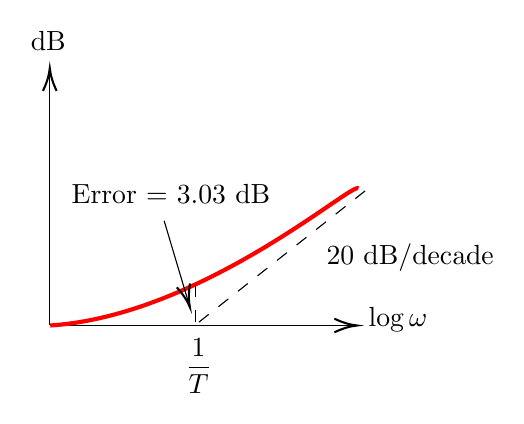
\begin{tikzpicture}[x=0.75pt,y=0.75pt,yscale=-1,xscale=1]
%uncomment if require: \path (0,300); %set diagram left start at 0, and has height of 300

%Straight Lines [id:da20219203487957138] 
\draw    (65.5,209.63) -- (65.5,87.66) ;
\draw [shift={(65.5,85.66)}, rotate = 450] [color={rgb, 255:red, 0; green, 0; blue, 0 }  ][line width=0.75]    (10.93,-3.29) .. controls (6.95,-1.4) and (3.31,-0.3) .. (0,0) .. controls (3.31,0.3) and (6.95,1.4) .. (10.93,3.29)   ;
%Straight Lines [id:da6575334279005483] 
\draw    (65.7,209.63) -- (211.55,209.63) ;
\draw [shift={(213.55,209.63)}, rotate = 180] [color={rgb, 255:red, 0; green, 0; blue, 0 }  ][line width=0.75]    (10.93,-3.29) .. controls (6.95,-1.4) and (3.31,-0.3) .. (0,0) .. controls (3.31,0.3) and (6.95,1.4) .. (10.93,3.29)   ;
%Straight Lines [id:da9896708874073339] 
\draw  [dash pattern={on 4.5pt off 4.5pt}]  (217.4,144.8) -- (135.83,209.2) ;
%Curve Lines [id:da1524138811680511] 
\draw [color={rgb, 255:red, 255; green, 0; blue, 0 }  ,draw opacity=1 ][line width=1.5]    (65.7,209.63) .. controls (139.2,204.8) and (212.2,139.6) .. (214.2,143.6) ;
%Straight Lines [id:da9088377067311144] 
\draw  [dash pattern={on 4.5pt off 4.5pt}]  (135.83,190) -- (135.83,209.2) ;
%Straight Lines [id:da2701365368475739] 
\draw    (120.6,159.2) -- (132.43,198.88) ;
\draw [shift={(133,200.8)}, rotate = 253.4] [color={rgb, 255:red, 0; green, 0; blue, 0 }  ][line width=0.75]    (10.93,-3.29) .. controls (6.95,-1.4) and (3.31,-0.3) .. (0,0) .. controls (3.31,0.3) and (6.95,1.4) .. (10.93,3.29)   ;

% Text Node
\draw (217.88,199.63) node [anchor=north west][inner sep=0.75pt]    {$\log \omega $};
% Text Node
\draw (55.11,66.41) node [anchor=north west][inner sep=0.75pt]   [align=left] {dB};
% Text Node
\draw (129.5,214.5) node [anchor=north west][inner sep=0.75pt]    {$\displaystyle\frac{1}{T}$};
% Text Node
\draw (74.8,140.4) node [anchor=north west][inner sep=0.75pt]   [align=left] {Error = 3.03 dB};
% Text Node
\draw (197.6,168.8) node [anchor=north west][inner sep=0.75pt]   [align=left] {20 dB/decade};


\end{tikzpicture}

    \end{center}
    \end{minipage}
    \begin{minipage}{0.55\textwidth}
    \item Phase: $\phi = \angle Tj\omega +1 = -\tan^{-1}\omega T$
    \begin{itemize}[label=$\circ$]
        \item At low frequency: $\phi\approx\tan^{-1}0 = 0^\circ$.
        \item At high frequency: $\phi \approx \tan^{-1} \infty = 90^\circ$.
        \item Asymptotes meet at corner frequency where $\omega = \displaystyle\frac{1}{T}$:\\
        $\phi = \tan^{-1} 1 = 45^\circ$
    \end{itemize}
    \end{minipage}
    \begin{minipage}{0.45\textwidth}
    \begin{center}
        \tikzset{every picture/.style={line width=0.75pt}} %set default line width to 0.75pt        
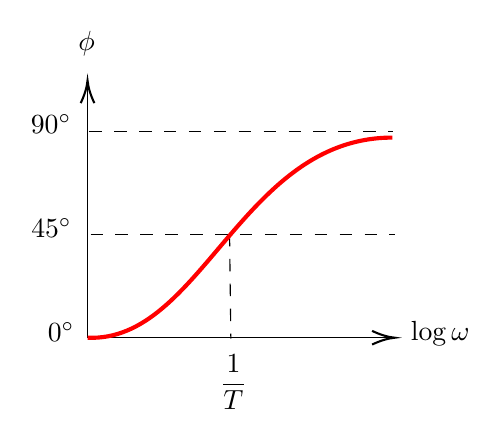
\begin{tikzpicture}[x=0.75pt,y=0.75pt,yscale=-1,xscale=1]
%Straight Lines [id:da41991018488295473] 
\draw    (371.76,199.22) -- (371.76,77.25) ;
\draw [shift={(371.76,75.25)}, rotate = 450] [color={rgb, 255:red, 0; green, 0; blue, 0 }  ][line width=0.75]    (10.93,-3.29) .. controls (6.95,-1.4) and (3.31,-0.3) .. (0,0) .. controls (3.31,0.3) and (6.95,1.4) .. (10.93,3.29)   ;
%Straight Lines [id:da9264184908369435] 
\draw    (371.76,199.22) -- (517.8,199.22) ;
\draw [shift={(519.8,199.22)}, rotate = 180] [color={rgb, 255:red, 0; green, 0; blue, 0 }  ][line width=0.75]    (10.93,-3.29) .. controls (6.95,-1.4) and (3.31,-0.3) .. (0,0) .. controls (3.31,0.3) and (6.95,1.4) .. (10.93,3.29)   ;
%Straight Lines [id:da9692637534102959] 
\draw  [dash pattern={on 4.5pt off 4.5pt}]  (373.2,149.4) -- (519.7,149.4) ;
%Straight Lines [id:da6463456321040173] 
\draw  [dash pattern={on 4.5pt off 4.5pt}]  (372.6,100) -- (519.1,100) ;
%Straight Lines [id:da6137764152272605] 
\draw  [dash pattern={on 4.5pt off 4.5pt}]  (440.2,149.2) -- (440.8,199.65) ;
%Curve Lines [id:da472769148646514] 
\draw [color={rgb, 255:red, 255; green, 0; blue, 0 }  ,draw opacity=1 ][line width=1.5]    (371.76,199.22) .. controls (426.6,201.6) and (446.1,102.8) .. (518.6,102.8) ;
% Text Node
\draw (366.09,50.11) node [anchor=north west][inner sep=0.75pt]    {$\phi $};
% Text Node
\draw (526.3,190.16) node [anchor=north west][inner sep=0.75pt]    {$\log \omega $};
% Text Node
\draw (343.19,90.5) node [anchor=north west][inner sep=0.75pt]    {$90^{\circ }$};
% Text Node
\draw (351.4,190.5) node [anchor=north west][inner sep=0.75pt]    {$0^{\circ }$};
% Text Node
\draw (343.4,140.5) node [anchor=north west][inner sep=0.75pt]    {$45^{\circ }$};
% Text Node
\draw (434.4,206) node [anchor=north west][inner sep=0.75pt]    {$\displaystyle\frac{1}{T}$};
\end{tikzpicture}
    \end{center}
    \end{minipage}
\end{itemize}

\newpage
\subsection{Bode Diagram of Second Order System}
$$G(j\omega) = \frac{\omega_n^2}{(j\omega)^2+2\zeta\omega_n(j\omega)+\omega_n^2} = \frac{1}{\left(j\frac{\omega}{\omega_n}\right)^2+2\zeta\left(j\frac{\omega}{\omega_n}\right)+1}$$
\begin{itemize}
    \item If system is overdamped ($\zeta > 1),\ G(j\omega)$ is a product of two first order systems.
    \item Magnitude when $0<\zeta<1$: 
    dB $= -20\log_{10}\sqrt{\left(1-\frac{\omega^2}{\omega_n^2}\right)^2+\left(2\zeta\frac{\omega}{\omega_n}\right)^2}$
    \begin{itemize}[label=$\circ$]
        \item At low frequency, $\omega\ll\omega_n,\ \text{dB}\approx 0$.
        \item At high frequency, $\omega\gg\omega_n,\ \text{dB}\approx -20\log_{10}\frac{\omega^2}{\omega_n^2} = -40\log_{10}\frac{\omega}{\omega_n}$ \quad (-40 dB/decade)
    \end{itemize}
    \item Phase when $0<\zeta<1: \phi = \tan^{-1}\displaystyle\frac{2\zeta\frac{\omega}{\omega_n}}{1-\left(\frac{\omega}{\omega_n}\right)^2}$
    \begin{itemize}[label=$\circ$]
        \item At low frequency, $\phi \approx 0^\circ$.
        \item At high frequency, $\phi\approx -\tan^{-1}\left(-\frac{\omega_n}{\omega}\right) = -180^\circ$.
        \item At corner frequency, $\phi = -\tan^{-1}\left(\frac{2\zeta}{0}\right)= -90^\circ$.
    \end{itemize}
\end{itemize}
\begin{minipage}{0.5\textwidth}
\begin{center}
\tikzset{every picture/.style={line width=0.75pt}} %set default line width to 0.75pt        
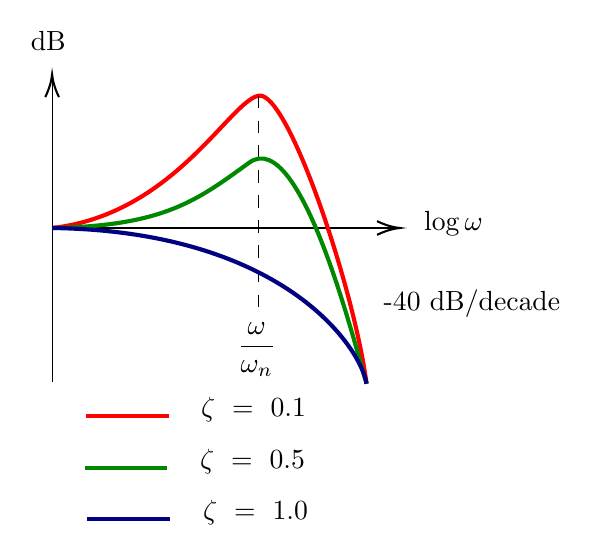
\begin{tikzpicture}[x=0.75pt,y=0.75pt,yscale=-1,xscale=1]
%Straight Lines [id:da39875375831471827] 
\draw    (100,218.75) -- (100,72.75) ;
\draw [shift={(100,70.75)}, rotate = 450] [color={rgb, 255:red, 0; green, 0; blue, 0 }  ][line width=0.75]    (10.93,-3.29) .. controls (6.95,-1.4) and (3.31,-0.3) .. (0,0) .. controls (3.31,0.3) and (6.95,1.4) .. (10.93,3.29)   ;
%Straight Lines [id:da9816341489394134] 
\draw    (100,144.75) -- (265.5,144.75) ;
\draw [shift={(267.5,144.75)}, rotate = 180] [color={rgb, 255:red, 0; green, 0; blue, 0 }  ][line width=0.75]    (10.93,-3.29) .. controls (6.95,-1.4) and (3.31,-0.3) .. (0,0) .. controls (3.31,0.3) and (6.95,1.4) .. (10.93,3.29)   ;
%Curve Lines [id:da44248437542364405] 
\draw [color={rgb, 255:red, 255; green, 0; blue, 0 }  ,draw opacity=1 ][line width=1.5]    (100,144.75) .. controls (158.5,138.25) and (185.5,83.75) .. (199.5,81) .. controls (213.5,78.25) and (245.5,173.75) .. (251.5,219.75) ;
%Straight Lines [id:da703280408751088] 
\draw  [dash pattern={on 4.5pt off 4.5pt}]  (199.5,81) -- (199.5,188.75) ;
%Curve Lines [id:da9548027566039015] 
\draw [color={rgb, 255:red, 0; green, 136; blue, 0 }  ,draw opacity=1 ][line width=1.5]    (100,144.75) .. controls (154.5,143.75) and (170,131.25) .. (195,113.25) .. controls (220,95.25) and (246.5,203.75) .. (251.5,219.75) ;
%Curve Lines [id:da988954111037625] 
\draw [color={rgb, 255:red, 0; green, 0; blue, 128 }  ,draw opacity=1 ][line width=1.5]    (100,144.75) .. controls (211,146.25) and (248.5,201.75) .. (251.5,219.75) ;
%Straight Lines [id:da06398443459899616] 
\draw [color={rgb, 255:red, 255; green, 0; blue, 0 }  ,draw opacity=1 ][line width=1.5]    (116.5,235.5) -- (156.5,235.5) ;
%Straight Lines [id:da3534454844567263] 
\draw [color={rgb, 255:red, 0; green, 136; blue, 0 }  ,draw opacity=1 ][line width=1.5]    (116,260.5) -- (155.5,260.5) ;
%Straight Lines [id:da7856824764479025] 
\draw [color={rgb, 255:red, 0; green, 0; blue, 128 }  ,draw opacity=1 ][line width=1.5]    (117,285) -- (157,285) ;
% Text Node
\draw (278,135.4) node [anchor=north west][inner sep=0.75pt]    {$\log \omega $};
% Text Node
\draw (88.5,48.5) node [anchor=north west][inner sep=0.75pt]   [align=left] {dB};
% Text Node
\draw (258.5,173) node [anchor=north west][inner sep=0.75pt]   [align=left] {\mbox{-}40 dB/decade};
% Text Node
\draw (170.5,224.9) node [anchor=north west][inner sep=0.75pt]    {$\zeta \ =\ 0.1$};
% Text Node
\draw (170,249.9) node [anchor=north west][inner sep=0.75pt]    {$\zeta \ =\ 0.5$};
% Text Node
\draw (171.5,274.9) node [anchor=north west][inner sep=0.75pt]    {$\zeta \ =\ 1.0$};
% Text Node
\draw (188,189) node [anchor=north west][inner sep=0.75pt]    {$\displaystyle\frac{\omega }{\omega _{n}}$};
\end{tikzpicture}
\end{center}
\end{minipage}
\begin{minipage}{0.5\textwidth}
\begin{center}
    \tikzset{every picture/.style={line width=0.75pt}} %set default line width to 0.75pt        
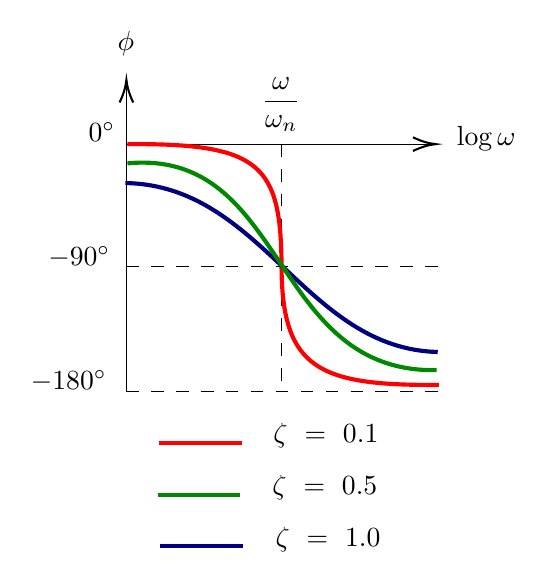
\begin{tikzpicture}[x=0.75pt,y=0.75pt,yscale=-1,xscale=1]
%Straight Lines [id:da3814026835173787] 
\draw    (100.5,179.75) -- (100.5,31.75) ;
\draw [shift={(100.5,29.75)}, rotate = 450] [color={rgb, 255:red, 0; green, 0; blue, 0 }  ][line width=0.75]    (10.93,-3.29) .. controls (6.95,-1.4) and (3.31,-0.3) .. (0,0) .. controls (3.31,0.3) and (6.95,1.4) .. (10.93,3.29)   ;
%Straight Lines [id:da7343759595254526] 
\draw    (101,60.75) -- (247.5,60.75) ;
\draw [shift={(249.5,60.75)}, rotate = 180] [color={rgb, 255:red, 0; green, 0; blue, 0 }  ][line width=0.75]    (10.93,-3.29) .. controls (6.95,-1.4) and (3.31,-0.3) .. (0,0) .. controls (3.31,0.3) and (6.95,1.4) .. (10.93,3.29)   ;
%Straight Lines [id:da47296080668461005] 
\draw  [dash pattern={on 4.5pt off 4.5pt}]  (100.5,119.5) -- (250.5,119.5) ;
%Straight Lines [id:da07466107490302565] 
\draw  [dash pattern={on 4.5pt off 4.5pt}]  (100.5,179.75) -- (250.5,179.75) ;
%Straight Lines [id:da4314511030916983] 
\draw  [dash pattern={on 4.5pt off 4.5pt}]  (175.25,60.75) -- (175.25,179.25) ;
%Curve Lines [id:da4485713306674415] 
\draw [color={rgb, 255:red, 255; green, 0; blue, 0 }  ,draw opacity=1 ][line width=1.5]    (101,60.75) .. controls (165.5,60.25) and (175,70.75) .. (175.25,120) .. controls (175.5,169.25) and (193.5,177.13) .. (251,176.75) ;
%Curve Lines [id:da47950431979036656] 
\draw [color={rgb, 255:red, 0; green, 0; blue, 128 }  ,draw opacity=1 ][line width=1.5]    (100,79.5) .. controls (166,80.5) and (186.5,159.38) .. (250.5,160.88) ;
%Curve Lines [id:da9638671351529977] 
\draw [color={rgb, 255:red, 0; green, 136; blue, 0 }  ,draw opacity=1 ][line width=1.5]    (101,70) .. controls (178.5,62.75) and (169.5,171.13) .. (250,169.63) ;
%Straight Lines [id:da11542994321006939] 
\draw [color={rgb, 255:red, 255; green, 0; blue, 0 }  ,draw opacity=1 ][line width=1.5]    (116.1,204.8) -- (156.1,204.8) ;
%Straight Lines [id:da0662410549277106] 
\draw [color={rgb, 255:red, 0; green, 136; blue, 0 }  ,draw opacity=1 ][line width=1.5]    (115.6,229.8) -- (155.1,229.8) ;
%Straight Lines [id:da28698733635607243] 
\draw [color={rgb, 255:red, 0; green, 0; blue, 128 }  ,draw opacity=1 ][line width=1.5]    (116.6,254.3) -- (156.6,254.3) ;
% Text Node
\draw (81,48.9) node [anchor=north west][inner sep=0.75pt]    {$0^{\circ }$};
% Text Node
\draw (164.5,27.4) node [anchor=north west][inner sep=0.75pt]    {$\displaystyle\frac{\omega }{\omega _{n}}$};
% Text Node
\draw (95,4.9) node [anchor=north west][inner sep=0.75pt]    {$\phi $};
% Text Node
\draw (258.5,50.9) node [anchor=north west][inner sep=0.75pt]    {$\log \omega $};
% Text Node
\draw (170.1,194.2) node [anchor=north west][inner sep=0.75pt]    {$\zeta \ =\ 0.1$};
% Text Node
\draw (169.6,219.2) node [anchor=north west][inner sep=0.75pt]    {$\zeta \ =\ 0.5$};
% Text Node
\draw (171.1,244.2) node [anchor=north west][inner sep=0.75pt]    {$\zeta \ =\ 1.0$};
% Text Node
\draw (61.6,108.6) node [anchor=north west][inner sep=0.75pt]    {$-90^{\circ }$};
% Text Node
\draw (53.2,168.4) node [anchor=north west][inner sep=0.75pt]    {$-180^{\circ }$};
\end{tikzpicture}
\end{center}
\end{minipage}
\begin{itemize}
    \item Maximum $|G(j\omega)|$ occurs when $g(\omega) = \left(1-\displaystyle\frac{\omega^2}{\omega_n^2}\right)^2 + \left(2\zeta\displaystyle\frac{\omega}{\omega_n}\right)^2$ is a minimum.
\end{itemize}
\begin{table}[H]
\centering\makegapedcells
\begin{tabular}{l|c|c|}
\cline{2-3}
                                                                                                        & \multicolumn{2}{c|}{\textbf{Damping ratio}, $\zeta$}                     \\ \cline{2-3} 
                                                                                                        & $0\leq\zeta\leq 0.707$                          & $\zeta>0.707$ \\ \hline
\multicolumn{1}{|l|}{\textbf{Resonant freq.}}                                                   & $\omega_n\sqrt{1-2\zeta^2}$                     & None          \\ \hline
\multicolumn{1}{|l|}{\begin{tabular}[c]{@{}l@{}}\textbf{Magnitude at} \\\textbf{resonant  freq.}\end{tabular}} & $\displaystyle\frac{1}{2\zeta\sqrt{1-\zeta^2}}$ & 1             \\ \hline
\end{tabular}
\end{table}

\newpage
\subsection{General Procedure for Drawing Bode Diagrams}
\begin{itemize}
    \item Decompose function into Bode Form.
\begin{align*}
    \text{e.g. }G(j\omega) &= \frac{10(j\omega+3)}{j\omega(j\omega+2)[(j\omega)^2+j\omega+2]}\\
    &= \frac{7.5\left(\frac{j\omega}{3}+1\right)}{j\omega\left(\frac{j\omega}{2}+1\right)\left[\frac{(j\omega)^2}{2}+\frac{j\omega}{2}+1\right]}
\end{align*}
    \item Identify corner frequency for each factor and construct asymptotes,
    \item Composite magnitude-frequency and phase-frequency plots are superposition of all individual magnitude-frequency and phase-frequency plots.
    \item e.g.
\begin{table}[H]
\centering\makegapedcells
\begin{tabular}{|l|c|c|c|c|c|}
\hline
\textbf{Bode form}        & 7.5 & $(j\omega)^{-1}$ & $1+j\displaystyle\frac{\omega}{3}$          & $\left(1+j\displaystyle\frac{\omega}{2}\right)^{-1}$ & $\left[1+j\displaystyle\frac{\omega}{2}+\frac{(j\omega)^2}{2}\right]^{-1}$ \\ \hline
\textbf{Corner frequency} & -   & -                & $T = \displaystyle\frac{1}{3},\ \omega = 3$ & $T = \displaystyle\frac{1}{2},\ \omega = 2$          & $\omega_n^2 = 2,\ \omega = \omega_n = \sqrt{2}$                            \\ \hline
\end{tabular}
\end{table}
\end{itemize}

\subsection{Minimum and Non-Minimum Phase Systems}
\begin{table}[H]
\centering
\begin{tabular}{l|c|c|}
\cline{2-3}
                                                                                                                                & \textbf{Minimum phase systems} & \textbf{Non-minimum phase systems}                                                 \\ \hline
\multicolumn{1}{|l|}{\textbf{Poles and zeros in RHP}}                                                                           & No                             & Yes                                                                                \\ \hline
\multicolumn{1}{|l|}{\textbf{Range in phase angle is minimum}}                                                                  & Yes                            & No                                                                                 \\ \hline
\multicolumn{1}{|l|}{\textbf{\begin{tabular}[c]{@{}l@{}}TF can be found from \\ magnitude-frequency plot\end{tabular}}}         & Yes                            & No                                                                                 \\ \hline
\multicolumn{1}{|l|}{\textbf{\begin{tabular}[c]{@{}l@{}}Slope at $\omega = \infty$ of\\ magnitude-frequency plot\end{tabular}}} & \multicolumn{2}{c|}{$-20(p-q)$ dB/decade}                                                                           \\ \hline
\multicolumn{1}{|l|}{\textbf{Phase angle at $\omega = 0$}}                                                                      & $-90^\circ(q-p)$               & \textcolor{red}{\textbf{NOT}} $-90^\circ(q-p)$ \\ \hline
\end{tabular}\\
\begin{center}
    where $p$ is the degree of the numerator polynomial in the TF,\\ and $q$ is the degree of the denominator polynomial in the TF.
\end{center}
\end{table}

\subsection{Interpreting Bode Diagrams}
\subsubsection{Type 0 System}
\begin{minipage}{0.4\textwidth}
\begin{center}
\tikzset{every picture/.style={line width=0.75pt}} %set default line width to 0.75pt        
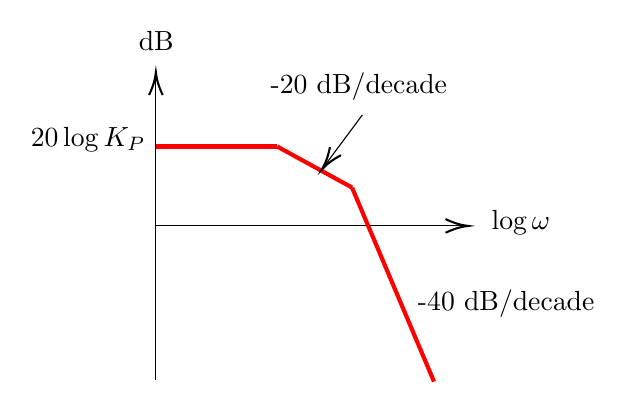
\begin{tikzpicture}[x=0.75pt,y=0.75pt,yscale=-1,xscale=1]
%Straight Lines [id:da9406899676643397] 
\draw    (156.5,239.75) -- (156.5,93.75) ;
\draw [shift={(156.5,91.75)}, rotate = 450] [color={rgb, 255:red, 0; green, 0; blue, 0 }  ][line width=0.75]    (10.93,-3.29) .. controls (6.95,-1.4) and (3.31,-0.3) .. (0,0) .. controls (3.31,0.3) and (6.95,1.4) .. (10.93,3.29)   ;
%Straight Lines [id:da03521485152855597] 
\draw    (156.5,165.75) -- (305,165.75) ;
\draw [shift={(307,165.75)}, rotate = 180] [color={rgb, 255:red, 0; green, 0; blue, 0 }  ][line width=0.75]    (10.93,-3.29) .. controls (6.95,-1.4) and (3.31,-0.3) .. (0,0) .. controls (3.31,0.3) and (6.95,1.4) .. (10.93,3.29)   ;
%Straight Lines [id:da37589405623576777] 
\draw [color={rgb, 255:red, 255; green, 0; blue, 0 }  ,draw opacity=1 ][line width=1.5]    (156.5,127.5) -- (215,127.5) ;
%Straight Lines [id:da3617194474673251] 
\draw [color={rgb, 255:red, 255; green, 0; blue, 0 }  ,draw opacity=1 ][line width=1.5]    (215,127.5) -- (251,147.25) ;
%Straight Lines [id:da4220083446658567] 
\draw [color={rgb, 255:red, 255; green, 0; blue, 0 }  ,draw opacity=1 ][line width=1.5]    (251,147.25) -- (290.5,240.75) ;
%Straight Lines [id:da8914349911002215] 
\draw    (256,112.25) -- (237.69,136.89) ;
\draw [shift={(236.5,138.5)}, rotate = 306.61] [color={rgb, 255:red, 0; green, 0; blue, 0 }  ][line width=0.75]    (10.93,-3.29) .. controls (6.95,-1.4) and (3.31,-0.3) .. (0,0) .. controls (3.31,0.3) and (6.95,1.4) .. (10.93,3.29)   ;
% Text Node
\draw (317,157) node [anchor=north west][inner sep=0.75pt]    {$\log \omega $};
% Text Node
\draw (147,70.5) node [anchor=north west][inner sep=0.75pt]   [align=left] {dB};
% Text Node
\draw (95,116.9) node [anchor=north west][inner sep=0.75pt]    {$20\log K_{P}$};
% Text Node
\draw (210.5,90.5) node [anchor=north west][inner sep=0.75pt]   [align=left] {\mbox{-}20 dB/decade};
% Text Node
\draw (281.5,195) node [anchor=north west][inner sep=0.75pt]   [align=left] {\mbox{-}40 dB/decade};
\end{tikzpicture}
\end{center}
\end{minipage}
\begin{minipage}{0.6\textwidth}
\begin{itemize}
    \item Horizontal line at low frequencies with value 20 $\log K_P$ dB
\end{itemize}
\end{minipage}

\newpage
\subsubsection{Type 1 System}
\begin{minipage}{0.4\textwidth}
\begin{center}
\tikzset{every picture/.style={line width=0.75pt}} %set default line width to 0.75pt        
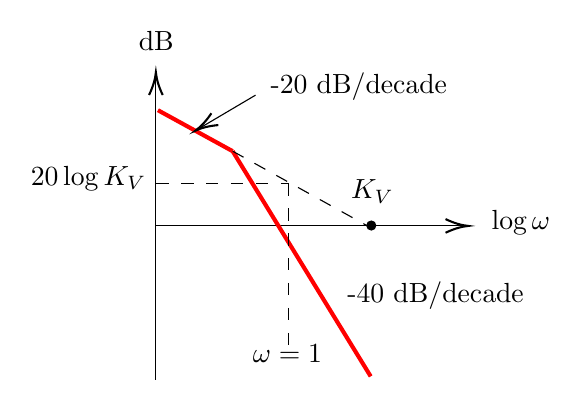
\begin{tikzpicture}[x=0.75pt,y=0.75pt,yscale=-1,xscale=1]
%uncomment if require: \path (0,300); %set diagram left start at 0, and has height of 300
%Straight Lines [id:da9406899676643397] 
\draw    (156.5,239.75) -- (156.5,93.75) ;
\draw [shift={(156.5,91.75)}, rotate = 450] [color={rgb, 255:red, 0; green, 0; blue, 0 }  ][line width=0.75]    (10.93,-3.29) .. controls (6.95,-1.4) and (3.31,-0.3) .. (0,0) .. controls (3.31,0.3) and (6.95,1.4) .. (10.93,3.29)   ;
%Straight Lines [id:da03521485152855597] 
\draw    (156.5,165.75) -- (305,165.75) ;
\draw [shift={(307,165.75)}, rotate = 180] [color={rgb, 255:red, 0; green, 0; blue, 0 }  ][line width=0.75]    (10.93,-3.29) .. controls (6.95,-1.4) and (3.31,-0.3) .. (0,0) .. controls (3.31,0.3) and (6.95,1.4) .. (10.93,3.29)   ;
%Straight Lines [id:da3617194474673251] 
\draw [color={rgb, 255:red, 255; green, 0; blue, 0 }  ,draw opacity=1 ][line width=1.5]    (157.5,110) -- (193.5,129.75) ;
%Straight Lines [id:da4220083446658567] 
\draw [color={rgb, 255:red, 255; green, 0; blue, 0 }  ,draw opacity=1 ][line width=1.5]    (193.5,129.75) -- (260,238.25) ;
%Straight Lines [id:da8914349911002215] 
\draw    (204.5,102.75) -- (177.22,118.86) ;
\draw [shift={(175.5,119.88)}, rotate = 329.44] [color={rgb, 255:red, 0; green, 0; blue, 0 }  ][line width=0.75]    (10.93,-3.29) .. controls (6.95,-1.4) and (3.31,-0.3) .. (0,0) .. controls (3.31,0.3) and (6.95,1.4) .. (10.93,3.29)   ;
%Straight Lines [id:da49570497865441165] 
\draw  [dash pattern={on 4.5pt off 4.5pt}]  (193.5,129.75) -- (258.11,165.56) ;
%Straight Lines [id:da010977467117893713] 
\draw  [dash pattern={on 4.5pt off 4.5pt}]  (156.67,145.22) -- (220.33,145.22) ;
%Straight Lines [id:da028102888927995062] 
\draw  [dash pattern={on 4.5pt off 4.5pt}]  (220.33,145.22) -- (220.33,225.11) ;
%Shape: Circle [id:dp5027901334992457] 
\draw  [fill={rgb, 255:red, 0; green, 0; blue, 0 }  ,fill opacity=1 ] (258.11,165.56) .. controls (258.11,164.36) and (259.08,163.39) .. (260.28,163.39) .. controls (261.47,163.39) and (262.44,164.36) .. (262.44,165.56) .. controls (262.44,166.75) and (261.47,167.72) .. (260.28,167.72) .. controls (259.08,167.72) and (258.11,166.75) .. (258.11,165.56) -- cycle ;
% Text Node
\draw (317,157) node [anchor=north west][inner sep=0.75pt]    {$\log \omega $};
% Text Node
\draw (147,70.5) node [anchor=north west][inner sep=0.75pt]   [align=left] {dB};
% Text Node
\draw (95,135.84) node [anchor=north west][inner sep=0.75pt]    {$20\log K_{V}$};
% Text Node
\draw (210.5,90.5) node [anchor=north west][inner sep=0.75pt]   [align=left] {\mbox{-}20 dB/decade};
% Text Node
\draw (247.5,191.5) node [anchor=north west][inner sep=0.75pt]   [align=left] {\mbox{-}40 dB/decade};
% Text Node
\draw (202,221.51) node [anchor=north west][inner sep=0.75pt]    {$\omega =1$};
% Text Node
\draw (249.33,142.4) node [anchor=north west][inner sep=0.75pt]    {$K_{V}$};
\end{tikzpicture}
\end{center}
\end{minipage}
\begin{minipage}{0.6\textwidth}
\begin{itemize}
    \item Initial slope of -20 dB/decade
    \item Intersection with 0 dB line has frequency $K_V$
\end{itemize}
\end{minipage}

\subsubsection{Type 2 System}
\begin{minipage}{0.4\textwidth}
\begin{center}
    \tikzset{every picture/.style={line width=0.75pt}} %set default line width to 0.75pt        
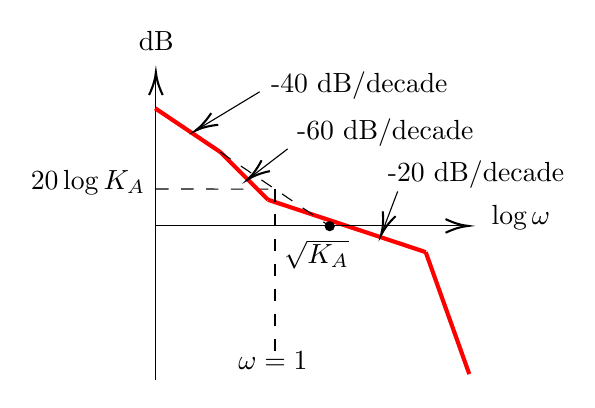
\begin{tikzpicture}[x=0.75pt,y=0.75pt,yscale=-1,xscale=1]
%Straight Lines [id:da5884349209744668] 
\draw [color={rgb, 255:red, 255; green, 0; blue, 0 }  ,draw opacity=1 ][line width=1.5]    (210.5,153.13) -- (286.5,178.38) ;
%Straight Lines [id:da9406899676643397] 
\draw    (156.5,239.75) -- (156.5,93.75) ;
\draw [shift={(156.5,91.75)}, rotate = 450] [color={rgb, 255:red, 0; green, 0; blue, 0 }  ][line width=0.75]    (10.93,-3.29) .. controls (6.95,-1.4) and (3.31,-0.3) .. (0,0) .. controls (3.31,0.3) and (6.95,1.4) .. (10.93,3.29)   ;
%Straight Lines [id:da03521485152855597] 
\draw    (156.5,165.75) -- (305,165.75) ;
\draw [shift={(307,165.75)}, rotate = 180] [color={rgb, 255:red, 0; green, 0; blue, 0 }  ][line width=0.75]    (10.93,-3.29) .. controls (6.95,-1.4) and (3.31,-0.3) .. (0,0) .. controls (3.31,0.3) and (6.95,1.4) .. (10.93,3.29)   ;
%Straight Lines [id:da4220083446658567] 
\draw [color={rgb, 255:red, 255; green, 0; blue, 0 }  ,draw opacity=1 ][line width=1.5]    (156.17,109.08) -- (187.5,130.13) ;
%Straight Lines [id:da8914349911002215] 
\draw    (206.5,101.13) -- (177.21,118.84) ;
\draw [shift={(175.5,119.88)}, rotate = 328.83000000000004] [color={rgb, 255:red, 0; green, 0; blue, 0 }  ][line width=0.75]    (10.93,-3.29) .. controls (6.95,-1.4) and (3.31,-0.3) .. (0,0) .. controls (3.31,0.3) and (6.95,1.4) .. (10.93,3.29)   ;
%Straight Lines [id:da010977467117893713] 
\draw  [dash pattern={on 4.5pt off 4.5pt}]  (156.67,147.97) -- (213.88,148) ;
%Straight Lines [id:da028102888927995062] 
\draw  [dash pattern={on 4.5pt off 4.5pt}]  (213.88,148) -- (213.88,227.89) ;
%Shape: Circle [id:dp5027901334992457] 
\draw  [fill={rgb, 255:red, 0; green, 0; blue, 0 }  ,fill opacity=1 ] (238.08,165.88) .. controls (238.08,164.68) and (239.05,163.71) .. (240.25,163.71) .. controls (241.45,163.71) and (242.42,164.68) .. (242.42,165.88) .. controls (242.42,167.07) and (241.45,168.04) .. (240.25,168.04) .. controls (239.05,168.04) and (238.08,167.07) .. (238.08,165.88) -- cycle ;
%Straight Lines [id:da22113486010946826] 
\draw [color={rgb, 255:red, 255; green, 0; blue, 0 }  ,draw opacity=1 ][line width=1.5]    (187.5,130.13) -- (210.5,153.13) ;
%Straight Lines [id:da019440638751194506] 
\draw [color={rgb, 255:red, 255; green, 0; blue, 0 }  ,draw opacity=1 ][line width=1.5]    (286.5,178.38) -- (307.5,237.13) ;
%Straight Lines [id:da5525618173572562] 
\draw  [dash pattern={on 4.5pt off 4.5pt}]  (187.5,130.13) -- (240.25,165.88) ;
%Straight Lines [id:da15081319308121488] 
\draw    (220,128.63) -- (202.34,142.16) ;
\draw [shift={(200.75,143.38)}, rotate = 322.53999999999996] [color={rgb, 255:red, 0; green, 0; blue, 0 }  ][line width=0.75]    (10.93,-3.29) .. controls (6.95,-1.4) and (3.31,-0.3) .. (0,0) .. controls (3.31,0.3) and (6.95,1.4) .. (10.93,3.29)   ;
%Straight Lines [id:da04699321726242012] 
\draw    (273,149.13) -- (265.71,168.26) ;
\draw [shift={(265,170.13)}, rotate = 290.85] [color={rgb, 255:red, 0; green, 0; blue, 0 }  ][line width=0.75]    (10.93,-3.29) .. controls (6.95,-1.4) and (3.31,-0.3) .. (0,0) .. controls (3.31,0.3) and (6.95,1.4) .. (10.93,3.29)   ;
% Text Node
\draw (317,154.4) node [anchor=north west][inner sep=0.75pt]    {$\log \omega $};
% Text Node
\draw (147,70.5) node [anchor=north west][inner sep=0.75pt]   [align=left] {dB};
% Text Node
\draw (95,137.84) node [anchor=north west][inner sep=0.75pt]    {$20\log K_{A}$};
% Text Node
\draw (210.75,90.25) node [anchor=north west][inner sep=0.75pt]   [align=left] {\mbox{-}40 dB/decade};
% Text Node
\draw (195,225.26) node [anchor=north west][inner sep=0.75pt]    {$\omega =1$};
% Text Node
\draw (217.08,171.4) node [anchor=north west][inner sep=0.75pt]    {$\sqrt{K_{A}}$};
% Text Node
\draw (223.25,113) node [anchor=north west][inner sep=0.75pt]   [align=left] {\mbox{-}60 dB/decade};
% Text Node
\draw (267,133.25) node [anchor=north west][inner sep=0.75pt]   [align=left] {\mbox{-}20 dB/decade};
\end{tikzpicture}
\end{center}
\end{minipage}
\begin{minipage}{0.6\textwidth}
\begin{itemize}
    \item Initial slope of -40 dB/decade
    \item Intersection with 0 dB line has frequency $\sqrt{K_A}$
\end{itemize}
\end{minipage}

\subsection{Stability Margins}
\begin{minipage}{0.4\textwidth}
\begin{center}
\tikzset{every picture/.style={line width=0.75pt}} %set default line width to 0.75pt        
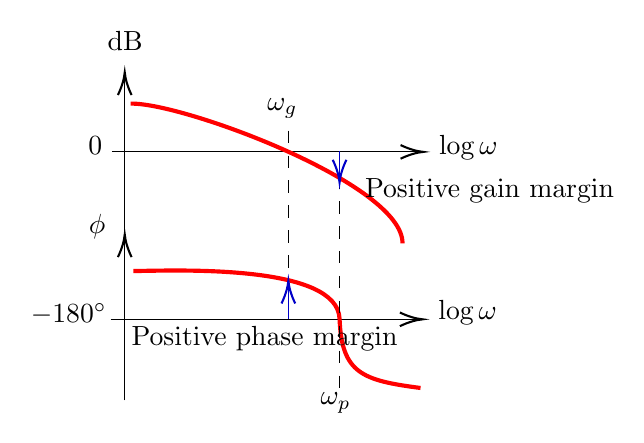
\begin{tikzpicture}[x=0.75pt,y=0.75pt,yscale=-1,xscale=1]
%Straight Lines [id:da9406899676643397] 
\draw    (156.5,239.75) -- (156.5,93.75) ;
\draw [shift={(156.5,91.75)}, rotate = 450] [color={rgb, 255:red, 0; green, 0; blue, 0 }  ][line width=0.75]    (10.93,-3.29) .. controls (6.95,-1.4) and (3.31,-0.3) .. (0,0) .. controls (3.31,0.3) and (6.95,1.4) .. (10.93,3.29)   ;
%Straight Lines [id:da03521485152855597] 
\draw    (150.33,130.08) -- (298.33,130.08) ;
\draw [shift={(300.33,130.08)}, rotate = 180] [color={rgb, 255:red, 0; green, 0; blue, 0 }  ][line width=0.75]    (10.93,-3.29) .. controls (6.95,-1.4) and (3.31,-0.3) .. (0,0) .. controls (3.31,0.3) and (6.95,1.4) .. (10.93,3.29)   ;
%Straight Lines [id:da6119370009462122] 
\draw    (156.5,249.83) -- (156.5,171.83) ;
\draw [shift={(156.5,169.83)}, rotate = 450] [color={rgb, 255:red, 0; green, 0; blue, 0 }  ][line width=0.75]    (10.93,-3.29) .. controls (6.95,-1.4) and (3.31,-0.3) .. (0,0) .. controls (3.31,0.3) and (6.95,1.4) .. (10.93,3.29)   ;
%Straight Lines [id:da7632095079385084] 
\draw    (149.67,210.75) -- (298,210.75) ;
\draw [shift={(300,210.75)}, rotate = 180] [color={rgb, 255:red, 0; green, 0; blue, 0 }  ][line width=0.75]    (10.93,-3.29) .. controls (6.95,-1.4) and (3.31,-0.3) .. (0,0) .. controls (3.31,0.3) and (6.95,1.4) .. (10.93,3.29)   ;
%Curve Lines [id:da0596605262588461] 
\draw [color={rgb, 255:red, 255; green, 0; blue, 0 }  ,draw opacity=1 ][line width=1.5]    (159.33,106.83) .. controls (184,106.17) and (290.67,145.5) .. (290.33,174.17) ;
%Curve Lines [id:da16259685033692994] 
\draw [color={rgb, 255:red, 255; green, 0; blue, 0 }  ,draw opacity=1 ][line width=1.5]    (160.67,187.5) .. controls (182.33,187.17) and (259,184.17) .. (260,210.5) .. controls (261,236.83) and (271,240.17) .. (299,243.83) ;
%Straight Lines [id:da5687658864952083] 
\draw  [dash pattern={on 4.5pt off 4.5pt}]  (235.33,119.83) -- (235.33,210.5) ;
%Straight Lines [id:da19880841933693905] 
\draw  [dash pattern={on 4.5pt off 4.5pt}]  (260,129.83) -- (260,248.17) ;
%Straight Lines [id:da8591259732864949] 
\draw [color={rgb, 255:red, 0; green, 0; blue, 200 }  ,draw opacity=1 ]   (260,129.83) -- (260,142.83) ;
\draw [shift={(260,144.83)}, rotate = 270] [color={rgb, 255:red, 0; green, 0; blue, 200 }  ,draw opacity=1 ][line width=0.75]    (10.93,-3.29) .. controls (6.95,-1.4) and (3.31,-0.3) .. (0,0) .. controls (3.31,0.3) and (6.95,1.4) .. (10.93,3.29)   ;
%Straight Lines [id:da5181583992869658] 
\draw [color={rgb, 255:red, 0; green, 0; blue, 200 }  ,draw opacity=1 ]   (235.33,210.5) -- (235.33,194.17) ;
\draw [shift={(235.33,192.17)}, rotate = 450] [color={rgb, 255:red, 0; green, 0; blue, 200 }  ,draw opacity=1 ][line width=0.75]    (10.93,-3.29) .. controls (6.95,-1.4) and (3.31,-0.3) .. (0,0) .. controls (3.31,0.3) and (6.95,1.4) .. (10.93,3.29)   ;
% Text Node
\draw (147,70.5) node [anchor=north west][inner sep=0.75pt]   [align=left] {dB};
% Text Node
\draw (138,159.07) node [anchor=north west][inner sep=0.75pt]    {$\phi $};
% Text Node
\draw (137.67,121.4) node [anchor=north west][inner sep=0.75pt]    {$0$};
% Text Node
\draw (110,202) node [anchor=north west][inner sep=0.75pt]    {$-180^{\circ }$};
% Text Node
\draw (306.67,120.73) node [anchor=north west][inner sep=0.75pt]    {$\log \omega $};
% Text Node
\draw (306.33,200.4) node [anchor=north west][inner sep=0.75pt]    {$\log \omega $};
% Text Node
\draw (224,103) node [anchor=north west][inner sep=0.75pt]    {$\omega _{g}$};
% Text Node
\draw (249.67,245) node [anchor=north west][inner sep=0.75pt]    {$\omega _{p}$};
% Text Node
\draw (271,141.83) node [anchor=north west][inner sep=0.75pt]   [align=left] {Positive gain margin};
% Text Node
\draw (158.5,212.83) node [anchor=north west][inner sep=0.75pt]   [align=left] {Positive phase margin};
\end{tikzpicture}
\end{center}
\end{minipage}
\begin{minipage}{0.6\textwidth}
\begin{itemize}
    \item \textbf{Gain Margin}, $K_g$: amount of gain that can be raised before instability, measured from phase-frequency plot
    \item \textbf{Phase Margin}, $\gamma$: amount of additional phase lag before instability, measured from magnitude-frequency plot
    \item \textbf{Gain crossover frequency}, $\omega_g$: frequency when dB = 0
    \item \textbf{Phase crossover frequency}, $\omega_p$: frequency when $\phi = -180^\circ$
\end{itemize}
\end{minipage}
\begin{itemize}
    \item If phase plot does not intersect $-180^\circ$, the gain margin is infinite.
    \item If magnitude plot does not intersect 0 dB, the phase margin is infinite.
    \item If both phase and gain margins are infinite, the system is absolutely stable.
\end{itemize}

\newpage
\section{W12: State Space Representation}
\begin{itemize}
    \item System organized as a set of first-order DEs
    \item ODEs do not need to be linear or time-invariant 
    \item Easily extended to MIMO systems
    \item Types of representations:
    \begin{itemize}[label=$\circ$]
        \item Non-linear, time varying \quad $\mathbf{\dot{x}}= f(\mathbf{x}, \mathbf{u}, t)\quad \mathbf{y} = g(\mathbf{x}, \mathbf{u}, t)$
        \item Linear time invariant \quad $\mathbf{\dot{x}} = \mathbf{Ax}+\mathbf{Bu} \quad \mathbf{y} = \mathbf{Cx}+\mathbf{Du}$
        \item Matrices and vectors:
    \end{itemize}
\end{itemize}
\begin{minipage}{0.33\textwidth}
\begin{align*}
    \text{State Vector, }\mathbf{x} = 
    \begin{bmatrix}
    x_1\\ \vdots\\ x_n
    \end{bmatrix}
\end{align*}
\end{minipage}
\begin{minipage}{0.34\textwidth}
\begin{align*}
    \text{Output Vector, }\mathbf{y} =
    \begin{bmatrix}
    y_1\\ \vdots\\ y_m
    \end{bmatrix}
\end{align*}
\end{minipage}
\begin{minipage}{0.33\textwidth}
\begin{align*}
    \text{Input Vector, }\mathbf{u} =
    \begin{bmatrix}
    u_1\\ \vdots\\ u_r
    \end{bmatrix}
\end{align*}
\end{minipage}

\begin{minipage}{0.25\textwidth}
\begin{align*}
    \mathbf{A} =
    \begin{bmatrix}
    a_{11} & \cdots & a_{1n}\\
    \vdots & \ddots & \vdots\\
    a_{n1} & \cdots & a_{nn}
    \end{bmatrix}
\end{align*}
\begin{center}
    State Matrix
\end{center}
\end{minipage}
\begin{minipage}{0.25\textwidth}
\begin{align*}
    \mathbf{B} = 
    \begin{bmatrix}
    b_{11} & \cdots & b_{1r}\\
    \vdots & \ddots & \vdots\\
    b_{n1} & \cdots & b_{nr}
    \end{bmatrix}
\end{align*}
\begin{center}
    Input Matrix
\end{center}
\end{minipage}
\begin{minipage}{0.25\textwidth}
\begin{align*}
    \mathbf{C} =
    \begin{bmatrix}
    c_{11} & \cdots & c_{1n}\\
    \vdots & \ddots & \vdots\\
    c_{m1} & \cdots & c_{mn}
    \end{bmatrix}
\end{align*}
\begin{center}
    Output Matrix
\end{center}
\end{minipage}
\begin{minipage}{0.25\textwidth}
\begin{align*}
    \mathbf{D} = 
    \begin{bmatrix}
    d_{11} & \cdots & d_{1r}\\
    \vdots & \ddots & \vdots\\
    d_{m1} & \cdots & d_{mr}
    \end{bmatrix}
\end{align*}
\begin{center}
    Direct Transmission\\Matrix
\end{center}
\end{minipage}
\begin{center}
    \begin{align*}
        \text{where }&n\text{ is the order of the system},\\
        &m\text{ is the no. of outputs},\\
        &r\text{ is the no. of inputs}.
    \end{align*}
\end{center}
\begin{itemize}
    \item State variables and state space representation are not unique
\end{itemize}

\subsection{Constructing State Space Models}
\begin{itemize}
    \item Define arbitrary state variables
    \begin{itemize}[label=$\circ$]
        \item Total order of system determines required number of state variables.
    \end{itemize}
\end{itemize}
\begin{minipage}{0.25\textwidth}
\tikzset{every picture/.style={line width=0.75pt}} %set default line width to 0.75pt        
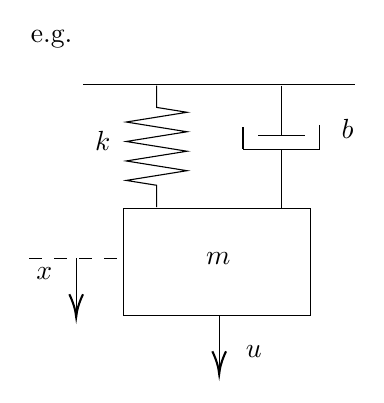
\begin{tikzpicture}[x=0.75pt,y=0.75pt,yscale=-1,xscale=1]
%uncomment if require: \path (0,300); %set diagram left start at 0, and has height of 300
%Straight Lines [id:da47280753828251965] 
\draw    (50.5,70.5) -- (181.5,70.5) ;
%Shape: Resistor [id:dp44430521180503413] 
\draw   (85.88,71) -- (85.88,81.55) -- (100.5,83.9) -- (71.25,88.59) -- (100.5,93.28) -- (71.25,97.97) -- (100.5,102.66) -- (71.25,107.35) -- (100.5,112.04) -- (71.25,116.73) -- (85.88,119.07) -- (85.88,129.63) ;
%Straight Lines [id:da6602110613400751] 
\draw    (146,71) -- (146,95.25) ;
%Straight Lines [id:da859019909125732] 
\draw    (134.75,95.25) -- (157.25,95.25) ;
%Straight Lines [id:da14082731390247716] 
\draw    (127.5,91) -- (127.5,101.75) ;
%Straight Lines [id:da7908712670747151] 
\draw    (127.5,101.75) -- (164.5,101.75) ;
%Straight Lines [id:da4754671583843235] 
\draw    (164.5,90) -- (164.5,101.75) ;
%Straight Lines [id:da8486598986005902] 
\draw    (146,101.75) -- (146,129.88) ;
%Shape: Rectangle [id:dp8853096197492674] 
\draw   (70,130.25) -- (160,130.25) -- (160,181.68) -- (70,181.68) -- cycle ;
%Straight Lines [id:da5423001190390058] 
\draw    (116,182) -- (116,208) ;
\draw [shift={(116,210)}, rotate = 270] [color={rgb, 255:red, 0; green, 0; blue, 0 }  ][line width=0.75]    (10.93,-3.29) .. controls (6.95,-1.4) and (3.31,-0.3) .. (0,0) .. controls (3.31,0.3) and (6.95,1.4) .. (10.93,3.29)   ;
%Straight Lines [id:da9897208974234626] 
\draw  [dash pattern={on 4.5pt off 4.5pt}]  (24.6,154.2) -- (69.6,154.2) ;
%Straight Lines [id:da6285769768732943] 
\draw    (47.1,154.2) -- (47.1,180.5) ;
\draw [shift={(47.1,182.5)}, rotate = 270] [color={rgb, 255:red, 0; green, 0; blue, 0 }  ][line width=0.75]    (10.93,-3.29) .. controls (6.95,-1.4) and (3.31,-0.3) .. (0,0) .. controls (3.31,0.3) and (6.95,1.4) .. (10.93,3.29)   ;
% Text Node
\draw (55,91.65) node [anchor=north west][inner sep=0.75pt]    {$k$};
% Text Node
\draw (173.75,86.15) node [anchor=north west][inner sep=0.75pt]    {$b$};
% Text Node
\draw (108.5,150) node [anchor=north west][inner sep=0.75pt]    {$m$};
% Text Node
\draw (127.6,194.8) node [anchor=north west][inner sep=0.75pt]    {$u$};
% Text Node
\draw (26.6,157.6) node [anchor=north west][inner sep=0.75pt]    {$x$};
% Text Node
\draw (24,43.4) node [anchor=north west][inner sep=0.75pt]   [align=left] {e.g.};
\end{tikzpicture}
\end{minipage}
\begin{minipage}{0.75\textwidth}
\begin{align*}
    \text{Equation of motion}:&\ m\ddot{x}+b\dot{x}+kx = u\\
    \text{State variables}:&\ x_1 =x,\quad x_2 = \dot{x}_1 = \dot{x}\\
    &\ \dot{x}_1 = x_2,\quad \dot{x}_2 = \ddot{x} = \frac{1}{m}(u-kx-b\dot{x})=\frac{1}{m}(u-kx_1-bx_2) 
\end{align*}
\begin{minipage}{0.3\textwidth}
\begin{center}
\begin{align*}
    \mathbf{\dot{x}} &= \mathbf{Ax} + \mathbf{Bu}\\
    \Rightarrow \begin{bmatrix}\dot{x}_1\\ \dot{x}_2\end{bmatrix} &= 
    \begin{bmatrix}0 & 1\\-\frac{k}{m}&-\frac{b}{m}\end{bmatrix}
    \begin{bmatrix}x_1\\x_2\end{bmatrix}+
    \begin{bmatrix}0\\ \frac{1}{m}\end{bmatrix}u
\end{align*}
\end{center}
\end{minipage}
\begin{minipage}{0.15\textwidth}
\quad
\end{minipage}
\begin{minipage}{0.3\textwidth}
\begin{center}
\begin{align*}
    \mathbf{y} &= \mathbf{Cx}+\mathbf{Du}\\
    \Rightarrow \begin{bmatrix}x_1\\x_2\end{bmatrix}&=
    \begin{bmatrix}1 & 0\end{bmatrix}
    \begin{bmatrix}x_1\\x_2\end{bmatrix},\
    \mathbf{D} = \begin{bmatrix}0\\0\end{bmatrix}
\end{align*}
\end{center}
\end{minipage}
\end{minipage}

\newpage
\subsection{Block Diagram Representation}
\begin{center}
    \tikzset{every picture/.style={line width=0.75pt}} %set default line width to 0.75pt        
\begin{tikzpicture}[x=0.75pt,y=0.75pt,yscale=-1,xscale=1]
%Shape: Rectangle [id:dp8953340175047348] 
\draw   (320.67,62.2) -- (390.67,62.2) -- (390.67,102.2) -- (320.67,102.2) -- cycle ;
%Shape: Rectangle [id:dp7447124491961425] 
\draw   (319.87,124.4) -- (389.87,124.4) -- (389.87,164.4) -- (319.87,164.4) -- cycle ;
%Shape: Rectangle [id:dp9111541956842104] 
\draw   (319.47,183.8) -- (389.47,183.8) -- (389.47,223.8) -- (319.47,223.8) -- cycle ;
\draw   (242.26,130.99) .. controls (248.12,125.14) and (257.62,125.14) .. (263.47,130.99) .. controls (269.33,136.85) and (269.33,146.35) .. (263.47,152.21) .. controls (257.62,158.06) and (248.12,158.06) .. (242.26,152.21) .. controls (236.4,146.35) and (236.4,136.85) .. (242.26,130.99) -- cycle ; \draw   (242.26,130.99) -- (263.47,152.21) ; \draw   (263.47,130.99) -- (242.26,152.21) ;
\draw   (239.64,141.37) -- (248.78,141.37)(244.21,136.8) -- (244.21,145.94) ;
\draw   (248.78,149.66) -- (257.92,149.66)(253.35,145.09) -- (253.35,154.23) ;
%Straight Lines [id:da18209432380161972] 
\draw    (268.07,142.37) -- (317.5,142.37) ;
\draw [shift={(319.5,142.37)}, rotate = 180] [color={rgb, 255:red, 0; green, 0; blue, 0 }  ][line width=0.75]    (10.93,-3.29) .. controls (6.95,-1.4) and (3.31,-0.3) .. (0,0) .. controls (3.31,0.3) and (6.95,1.4) .. (10.93,3.29)   ;
%Straight Lines [id:da7459298632524147] 
\draw    (253.35,202.8) -- (253.35,158.8) ;
\draw [shift={(253.35,156.8)}, rotate = 450] [color={rgb, 255:red, 0; green, 0; blue, 0 }  ][line width=0.75]    (10.93,-3.29) .. controls (6.95,-1.4) and (3.31,-0.3) .. (0,0) .. controls (3.31,0.3) and (6.95,1.4) .. (10.93,3.29)   ;
%Straight Lines [id:da2288072176946263] 
\draw    (253.35,202.8) -- (319.21,202.8) ;
%Shape: Rectangle [id:dp5720951629850555] 
\draw   (106.38,123.63) -- (176.38,123.63) -- (176.38,163.63) -- (106.38,163.63) -- cycle ;
%Straight Lines [id:da17251274930399618] 
\draw    (176.5,142.8) -- (235.5,142.8) ;
\draw [shift={(237.5,142.8)}, rotate = 180] [color={rgb, 255:red, 0; green, 0; blue, 0 }  ][line width=0.75]    (10.93,-3.29) .. controls (6.95,-1.4) and (3.31,-0.3) .. (0,0) .. controls (3.31,0.3) and (6.95,1.4) .. (10.93,3.29)   ;
%Straight Lines [id:da35715213045951844] 
\draw    (61.67,80.8) -- (318.47,80.8) ;
\draw [shift={(320.47,80.8)}, rotate = 180] [color={rgb, 255:red, 0; green, 0; blue, 0 }  ][line width=0.75]    (10.93,-3.29) .. controls (6.95,-1.4) and (3.31,-0.3) .. (0,0) .. controls (3.31,0.3) and (6.95,1.4) .. (10.93,3.29)   ;
%Straight Lines [id:da7660093019014753] 
\draw    (29.27,144.4) -- (104.07,144.4) ;
\draw [shift={(106.07,144.4)}, rotate = 180] [color={rgb, 255:red, 0; green, 0; blue, 0 }  ][line width=0.75]    (10.93,-3.29) .. controls (6.95,-1.4) and (3.31,-0.3) .. (0,0) .. controls (3.31,0.3) and (6.95,1.4) .. (10.93,3.29)   ;
%Straight Lines [id:da684849342538405] 
\draw    (61.67,80.8) -- (61.67,144.4) ;
%Shape: Rectangle [id:dp7062684332678237] 
\draw   (469.58,123.76) -- (539.58,123.76) -- (539.58,163.76) -- (469.58,163.76) -- cycle ;
%Straight Lines [id:da5185924523978289] 
\draw    (390.07,143) -- (467.27,143) ;
\draw [shift={(469.27,143)}, rotate = 180] [color={rgb, 255:red, 0; green, 0; blue, 0 }  ][line width=0.75]    (10.93,-3.29) .. controls (6.95,-1.4) and (3.31,-0.3) .. (0,0) .. controls (3.31,0.3) and (6.95,1.4) .. (10.93,3.29)   ;
%Straight Lines [id:da5545728625687505] 
\draw    (429.67,202.8) -- (391.27,202.8) ;
\draw [shift={(389.27,202.8)}, rotate = 360] [color={rgb, 255:red, 0; green, 0; blue, 0 }  ][line width=0.75]    (10.93,-3.29) .. controls (6.95,-1.4) and (3.31,-0.3) .. (0,0) .. controls (3.31,0.3) and (6.95,1.4) .. (10.93,3.29)   ;
%Straight Lines [id:da32759695429567937] 
\draw    (429.67,143) -- (429.67,203.2) ;
\draw   (587.26,133.33) .. controls (593.12,127.47) and (602.62,127.47) .. (608.47,133.33) .. controls (614.33,139.18) and (614.33,148.68) .. (608.47,154.54) .. controls (602.62,160.4) and (593.12,160.4) .. (587.26,154.54) .. controls (581.4,148.68) and (581.4,139.18) .. (587.26,133.33) -- cycle ; \draw   (587.26,133.33) -- (608.47,154.54) ; \draw   (608.47,133.33) -- (587.26,154.54) ;
\draw   (584.64,143.7) -- (593.78,143.7)(589.21,139.13) -- (589.21,148.28) ;
\draw   (594.11,135.66) -- (603.26,135.66)(598.69,131.09) -- (598.69,140.23) ;
%Straight Lines [id:da8525359178596501] 
\draw    (539.67,144) -- (581.33,144) ;
\draw [shift={(583.33,144)}, rotate = 180] [color={rgb, 255:red, 0; green, 0; blue, 0 }  ][line width=0.75]    (10.93,-3.29) .. controls (6.95,-1.4) and (3.31,-0.3) .. (0,0) .. controls (3.31,0.3) and (6.95,1.4) .. (10.93,3.29)   ;
%Straight Lines [id:da6335111572011627] 
\draw    (598.67,82.83) -- (598.67,126.67) ;
\draw [shift={(598.67,128.67)}, rotate = 270] [color={rgb, 255:red, 0; green, 0; blue, 0 }  ][line width=0.75]    (10.93,-3.29) .. controls (6.95,-1.4) and (3.31,-0.3) .. (0,0) .. controls (3.31,0.3) and (6.95,1.4) .. (10.93,3.29)   ;
%Straight Lines [id:da9542714108999892] 
\draw    (391.33,83) -- (598.67,83) ;
%Straight Lines [id:da0748350834738305] 
\draw    (614,144.33) -- (652.33,144.33) ;
\draw [shift={(654.33,144.33)}, rotate = 180] [color={rgb, 255:red, 0; green, 0; blue, 0 }  ][line width=0.75]    (10.93,-3.29) .. controls (6.95,-1.4) and (3.31,-0.3) .. (0,0) .. controls (3.31,0.3) and (6.95,1.4) .. (10.93,3.29)   ;
% Text Node
\draw (347.75,75) node [anchor=north west][inner sep=0.75pt]    {$\mathbf{D}$};
% Text Node
\draw (348,129) node [anchor=north west][inner sep=0.75pt]    {$\displaystyle\frac{1}{s}$};
% Text Node
\draw (348.27,194.4) node [anchor=north west][inner sep=0.75pt]    {$\mathbf{A}$};
% Text Node
\draw (134.7,137) node [anchor=north west][inner sep=0.75pt]    {$\mathbf{B}$};
% Text Node
\draw (11.47,137) node [anchor=north west][inner sep=0.75pt]    {$\mathbf{u}$};
% Text Node
\draw (497.9,137) node [anchor=north west][inner sep=0.75pt]    {$\mathbf{C}$};
% Text Node
\draw (659.33,137) node [anchor=north west][inner sep=0.75pt]    {$\mathbf{y}$};
% Text Node
\draw (425.33,122) node [anchor=north west][inner sep=0.75pt]    {$\mathbf{x}$};
% Text Node
\draw (282.67,122) node [anchor=north west][inner sep=0.75pt]    {$\dot{\mathbf{x}}$};
\end{tikzpicture}
\end{center}
\begin{align*}
    \mathbf{\dot{x}} &= \mathbf{Ax}+\mathbf{Bu}\\
    \mathbf{y} &= \mathbf{Cx}+\mathbf{Du}
\end{align*}

\subsection{Transfer Matrix}
Taking Laplace Transform:
\begin{align*}
    s\mathbf{X}(s)-\mathbf{x}(0) &= \mathbf{AX}(s)+\mathbf{BU}(s)\\
    \mathbf{Y}(s) &= \mathbf{CX}(s) +\mathbf{DU}(s)
\end{align*}
Zero initial conditions:
\begin{align*}
    s\mathbf{X}(s) &= \mathbf{AX}(s)+\mathbf{BU}(s)\\
    (s\mathbf{I}-\mathbf{A})\mathbf{X}(s) &= \mathbf{BU}(s)\\
    \mathbf{X(s)} &= (s\mathbf{I}-\mathbf{A})^{-1}\mathbf{BU}(s)
\end{align*}
Substituting $\mathbf{X}$(s) into $\mathbf{Y}$(s):
\begin{align*}
    \mathbf{Y}(s) &= \mathbf{C}\left[(s\mathbf{I}-\mathbf{A})^{-1}\mathbf{BU}(s)\right]+\mathbf{DU}(s)\\
    &= \mathbf{C}\left[(s\mathbf{I}-\mathbf{A})^{-1}\mathbf{B}+\mathbf{D}\right]\mathbf{U}(s)\\
    \Rightarrow \mathbf{G}(s) &= \frac{\mathbf{Y}(s)}{\mathbf{U}(s)}\\
    &= \mathbf{C}(s\mathbf{I}-\mathbf{A})^{-1}\mathbf{B}+\mathbf{D}
\end{align*}

\subsection{Eigenvalues and Characteristic Equation}
\begin{itemize}
    \item Characteristic equation: $|s\mathbf{I}-\mathbf{A}| = 0$
    \item Eigenvalues of $\mathbf{A}$ are roots of the characteristic equation
    \item Eigenvalues are not affected by linear transformations applied to $\mathbf{A}$
\end{itemize}

\newpage
\subsection{Stability Analysis in State-Space}
\begin{itemize}
    \item LTI State-Space System is stable if all eigenvalues have negative real parts
    \item Types of stability:
    \begin{itemize}[label=$\circ$]
        \item Absolute/ internal stability: LHP eigenvalues/poles
        \item Neutral stability: Non-repeated $j\omega$ axis poles
        \item Unstable: Repeated $j\omega$ axis poles, RHP eigenvalues/poles
    \end{itemize}
\end{itemize}

\newpage
\section{W13: Full State Feedback Control}
\begin{itemize}
    \item State space representation in W12 is an example of Open Loop Control, where $\mathbf{D}=0$
\end{itemize}
\begin{center}
\tikzset{every picture/.style={line width=0.75pt}} %set default line width to 0.75pt        
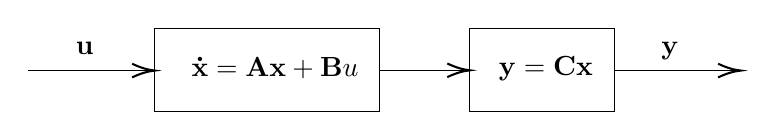
\begin{tikzpicture}[x=0.75pt,y=0.75pt,yscale=-1,xscale=1]
%Shape: Rectangle [id:dp7447124491961425] 
\draw   (93.2,129.4) -- (201.67,129.4) -- (201.67,169.4) -- (93.2,169.4) -- cycle ;
%Shape: Rectangle [id:dp7062684332678237] 
\draw   (244.91,129.43) -- (314.91,129.43) -- (314.91,169.43) -- (244.91,169.43) -- cycle ;
%Straight Lines [id:da8525359178596501] 
\draw    (201.67,149.67) -- (243.33,149.67) ;
\draw [shift={(245.33,149.67)}, rotate = 180] [color={rgb, 255:red, 0; green, 0; blue, 0 }  ][line width=0.75]    (10.93,-3.29) .. controls (6.95,-1.4) and (3.31,-0.3) .. (0,0) .. controls (3.31,0.3) and (6.95,1.4) .. (10.93,3.29)   ;
%Straight Lines [id:da47503718645482307] 
\draw    (32.5,149.8) -- (91.5,149.8) ;
\draw [shift={(93.5,149.8)}, rotate = 180] [color={rgb, 255:red, 0; green, 0; blue, 0 }  ][line width=0.75]    (10.93,-3.29) .. controls (6.95,-1.4) and (3.31,-0.3) .. (0,0) .. controls (3.31,0.3) and (6.95,1.4) .. (10.93,3.29)   ;
%Straight Lines [id:da5910393611367957] 
\draw    (314.83,149.8) -- (373.83,149.8) ;
\draw [shift={(375.83,149.8)}, rotate = 180] [color={rgb, 255:red, 0; green, 0; blue, 0 }  ][line width=0.75]    (10.93,-3.29) .. controls (6.95,-1.4) and (3.31,-0.3) .. (0,0) .. controls (3.31,0.3) and (6.95,1.4) .. (10.93,3.29)   ;
% Text Node
\draw (54.13,135) node [anchor=north west][inner sep=0.75pt]    {$\mathbf{u}$};
% Text Node
\draw (258,142) node [anchor=north west][inner sep=0.75pt]    {$\mathbf{y=Cx}$};
% Text Node
\draw (336.33,135) node [anchor=north west][inner sep=0.75pt]    {$\mathbf{y}$};
% Text Node
\draw (110,142) node [anchor=north west][inner sep=0.75pt]    {$\mathbf{\dot{x}} =\mathbf{Ax} +\mathbf{B} u$};
\end{tikzpicture}\\
{$\text{Characteristic equation: } |s\mathbf{I} -\mathbf{A}|=0$}
\end{center}
\begin{itemize}
    \item Full state feedback control can be achieved by adding feedback to the input:
    \begin{center}
        \tikzset{every picture/.style={line width=0.75pt}} %set default line width to 0.75pt        

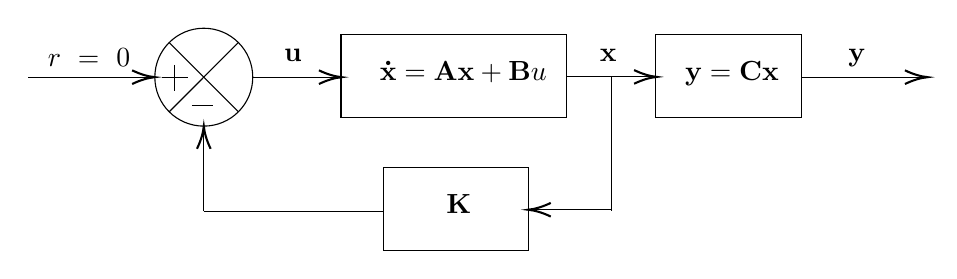
\begin{tikzpicture}[x=0.75pt,y=0.75pt,yscale=-1,xscale=1]
%uncomment if require: \path (0,300); %set diagram left start at 0, and has height of 300

%Shape: Rectangle [id:dp7447124491961425] 
\draw   (227.53,114.4) -- (336,114.4) -- (336,154.4) -- (227.53,154.4) -- cycle ;
%Shape: Rectangle [id:dp7062684332678237] 
\draw   (379.25,114.43) -- (449.25,114.43) -- (449.25,154.43) -- (379.25,154.43) -- cycle ;
%Straight Lines [id:da8525359178596501] 
\draw    (336,134.67) -- (377.67,134.67) ;
\draw [shift={(379.67,134.67)}, rotate = 180] [color={rgb, 255:red, 0; green, 0; blue, 0 }  ][line width=0.75]    (10.93,-3.29) .. controls (6.95,-1.4) and (3.31,-0.3) .. (0,0) .. controls (3.31,0.3) and (6.95,1.4) .. (10.93,3.29)   ;
%Straight Lines [id:da47503718645482307] 
\draw    (185,134.8) -- (225.83,134.8) ;
\draw [shift={(227.83,134.8)}, rotate = 180] [color={rgb, 255:red, 0; green, 0; blue, 0 }  ][line width=0.75]    (10.93,-3.29) .. controls (6.95,-1.4) and (3.31,-0.3) .. (0,0) .. controls (3.31,0.3) and (6.95,1.4) .. (10.93,3.29)   ;
%Straight Lines [id:da5910393611367957] 
\draw    (449.16,134.8) -- (508.16,134.8) ;
\draw [shift={(510.16,134.8)}, rotate = 180] [color={rgb, 255:red, 0; green, 0; blue, 0 }  ][line width=0.75]    (10.93,-3.29) .. controls (6.95,-1.4) and (3.31,-0.3) .. (0,0) .. controls (3.31,0.3) and (6.95,1.4) .. (10.93,3.29)   ;
%Shape: Rectangle [id:dp7717318983802177] 
\draw   (247.91,178.43) -- (317.91,178.43) -- (317.91,218.43) -- (247.91,218.43) -- cycle ;
%Straight Lines [id:da6581738651116429] 
\draw    (357.83,198.67) -- (319.67,198.67) ;
\draw [shift={(317.67,198.67)}, rotate = 360] [color={rgb, 255:red, 0; green, 0; blue, 0 }  ][line width=0.75]    (10.93,-3.29) .. controls (6.95,-1.4) and (3.31,-0.3) .. (0,0) .. controls (3.31,0.3) and (6.95,1.4) .. (10.93,3.29)   ;
%Straight Lines [id:da5427150423582097] 
\draw    (357.83,134.67) -- (357.83,199.17) ;
%Flowchart: Summing Junction [id:dp23127951205691266] 
\draw   (137.83,134.8) .. controls (137.83,121.78) and (148.39,111.22) .. (161.42,111.22) .. controls (174.44,111.22) and (185,121.78) .. (185,134.8) .. controls (185,147.82) and (174.44,158.38) .. (161.42,158.38) .. controls (148.39,158.38) and (137.83,147.82) .. (137.83,134.8) -- cycle ; \draw   (144.74,118.12) -- (178.09,151.48) ; \draw   (178.09,118.12) -- (144.74,151.48) ;
%Straight Lines [id:da9077307842571523] 
\draw    (76.83,134.8) -- (135.83,134.8) ;
\draw [shift={(137.83,134.8)}, rotate = 180] [color={rgb, 255:red, 0; green, 0; blue, 0 }  ][line width=0.75]    (10.93,-3.29) .. controls (6.95,-1.4) and (3.31,-0.3) .. (0,0) .. controls (3.31,0.3) and (6.95,1.4) .. (10.93,3.29)   ;
%Straight Lines [id:da5693384601129177] 
\draw    (155.67,148.33) -- (165.67,148.33) ;
\draw   (141.17,135.08) -- (153.67,135.08)(147.42,128.83) -- (147.42,141.33) ;
%Straight Lines [id:da6111442089765122] 
\draw    (161.42,199.5) -- (161.42,160.38) ;
\draw [shift={(161.42,158.38)}, rotate = 450] [color={rgb, 255:red, 0; green, 0; blue, 0 }  ][line width=0.75]    (10.93,-3.29) .. controls (6.95,-1.4) and (3.31,-0.3) .. (0,0) .. controls (3.31,0.3) and (6.95,1.4) .. (10.93,3.29)   ;
%Straight Lines [id:da17066253820117727] 
\draw    (161.42,199.5) -- (248,199.5) ;

% Text Node
\draw (198.8,120) node [anchor=north west][inner sep=0.75pt]    {$\mathbf{u}$};
% Text Node
\draw (392,126) node [anchor=north west][inner sep=0.75pt]    {$\mathbf{y=Cx}$};
% Text Node
\draw (470.67,120) node [anchor=north west][inner sep=0.75pt]    {$\mathbf{y}$};
% Text Node
\draw (245,126) node [anchor=north west][inner sep=0.75pt]    {$\mathbf{\dot{x}} =\mathbf{Ax} +\mathbf{B} u$};
% Text Node
\draw (277,190) node [anchor=north west][inner sep=0.75pt]    {$\mathbf{K}$};
% Text Node
\draw (351,120) node [anchor=north west][inner sep=0.75pt]    {$\mathbf{x}$};
% Text Node
\draw (85,120) node [anchor=north west][inner sep=0.75pt]    {$r\ =\ 0$};
\end{tikzpicture}\\
Characteristic equation: $|s\mathbf{I}-(\mathbf{A}-\mathbf{BK})| = 0$\\
Regulator control, $r = 0$\\
Control Law: $u = -\mathbf{Kx} = -k_1x_1-k_2x_2-k_3x_3-\cdots-k_nx_n$
\end{center}
\end{itemize}

\subsection{Motivation}
\begin{itemize}
    \item Location of open loop poles/eigenvalues of state-space system dictate stability and transient response
    \item Using feedback control, the closed loop poles can be placed where we want them to be in the $s$-plane.
\end{itemize}

\subsection{Pole Placement Controller Design}
\begin{enumerate}
    \item Check if possible to design such a controller.
    \begin{itemize}[label=$\circ$]
        \item Covered in 30.114
        \item If system can be designed, gain matrix $\mathbf{K} = [k_1\ k_2\ \cdots\ k_n]$.
        \item Control Law: $u= -\mathbf{Kx}$
    \end{itemize}
    \item Find desired closed loop performance using system parameters.
    \begin{itemize}[label=$\circ$]
        \item First Order System: Time constant $T, \text{ where } p=-\displaystyle\frac{1}{T}$ 
        \item Second Order System: Damping ratio $\zeta$ and natural frequency $\omega_n$
        \begin{center}
            $(s-p_1)(s-p_2) = s^2+2\zeta\omega_n s+\omega_n^2 = 0$\vspace{0.2cm}\\
            where $\zeta = \left[1+\left(\displaystyle\frac{\pi}{M_p}\right)^2\right]^{-0.5},\ \omega_n = \displaystyle\frac{\pi}{t_p\sqrt{1-\zeta^2}}$.
        \end{center}
       
        \item Underdamped $(0<\zeta<1)$, critically damped ($\zeta = 1$), overdamped ($\zeta>1$)
    \end{itemize}
    \item Find required controller gain $\mathbf{K}$ by equating desired CE with closed loop CE.
    $$\text{Desired CE} = |s\mathbf{I}-\mathbf{A}+\mathbf{BK}|=0$$
\end{enumerate}

\newpage
\subsection{Additional Notes}
\begin{itemize}
    \item Regulator system: constant reference input
    \item Control system: time-varying reference input
    \item Placing poles increasingly far away from the $j\omega$ axis results in exponentially larger input signals
    \begin{itemize}[label=$\circ$]
        \item System may become linear
        \item Require larger and heavier actuators
    \end{itemize}
    \item Alternative method: Quadratic Optimal Control (covered in 30.114)
    \item Gain matrix $\mathbf{K}$ is not unique to systems, dependent on location of closed loop poles
    \item May be optimal to use computer simulations instead for higher order systems
\end{itemize}
\end{document}